\clearpage

%%%%%%%%%%% DIST %%%%%%%%%%%%%%%%%%%
\begin{figure}
  \centering
  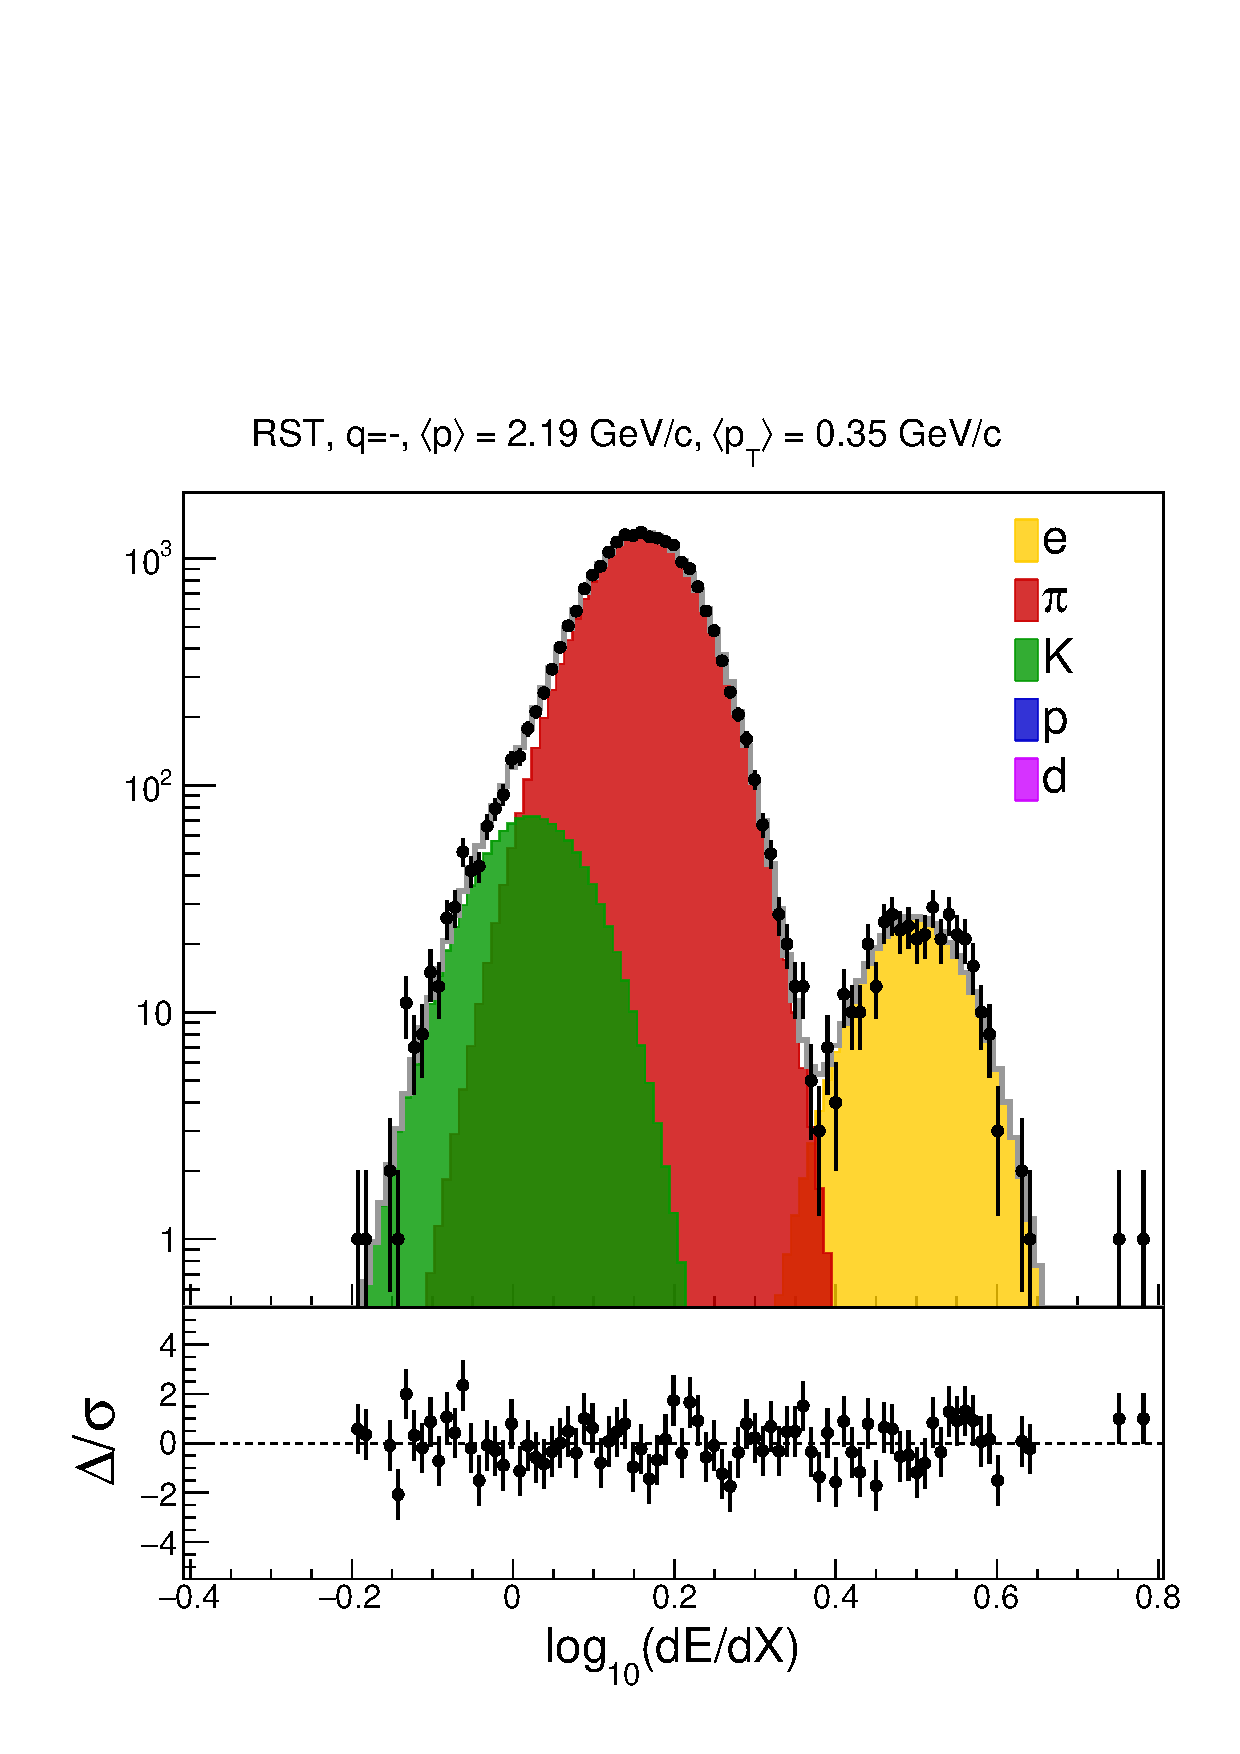
\includegraphics[clip, rviewport=0 0 1 1,width=0.4\textwidth]{dedx/dist_350_v0_c0_x13_y3}
  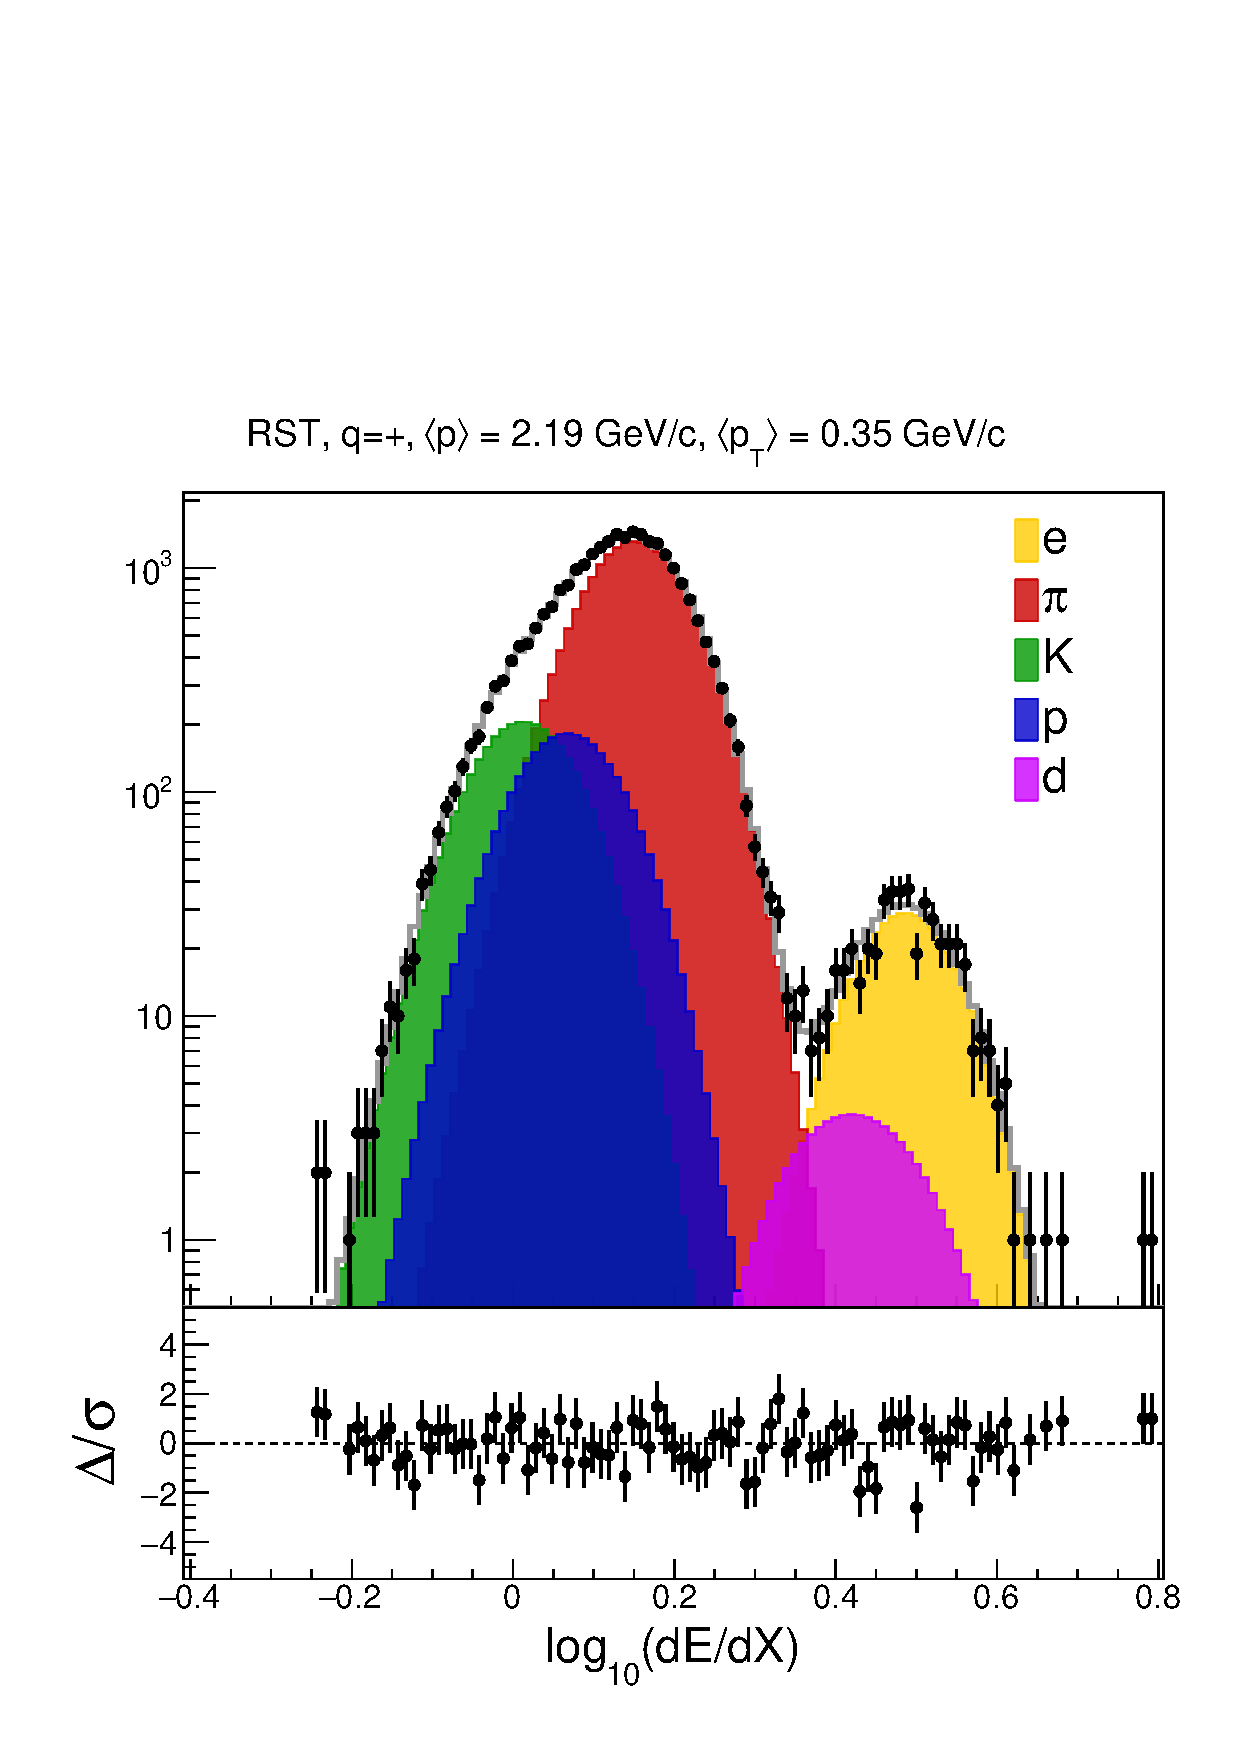
\includegraphics[clip, rviewport=0 0 1 1,width=0.4\textwidth]{dedx/dist_350_v0_c1_x13_y3}

  \vspace{0.5cm}
  
  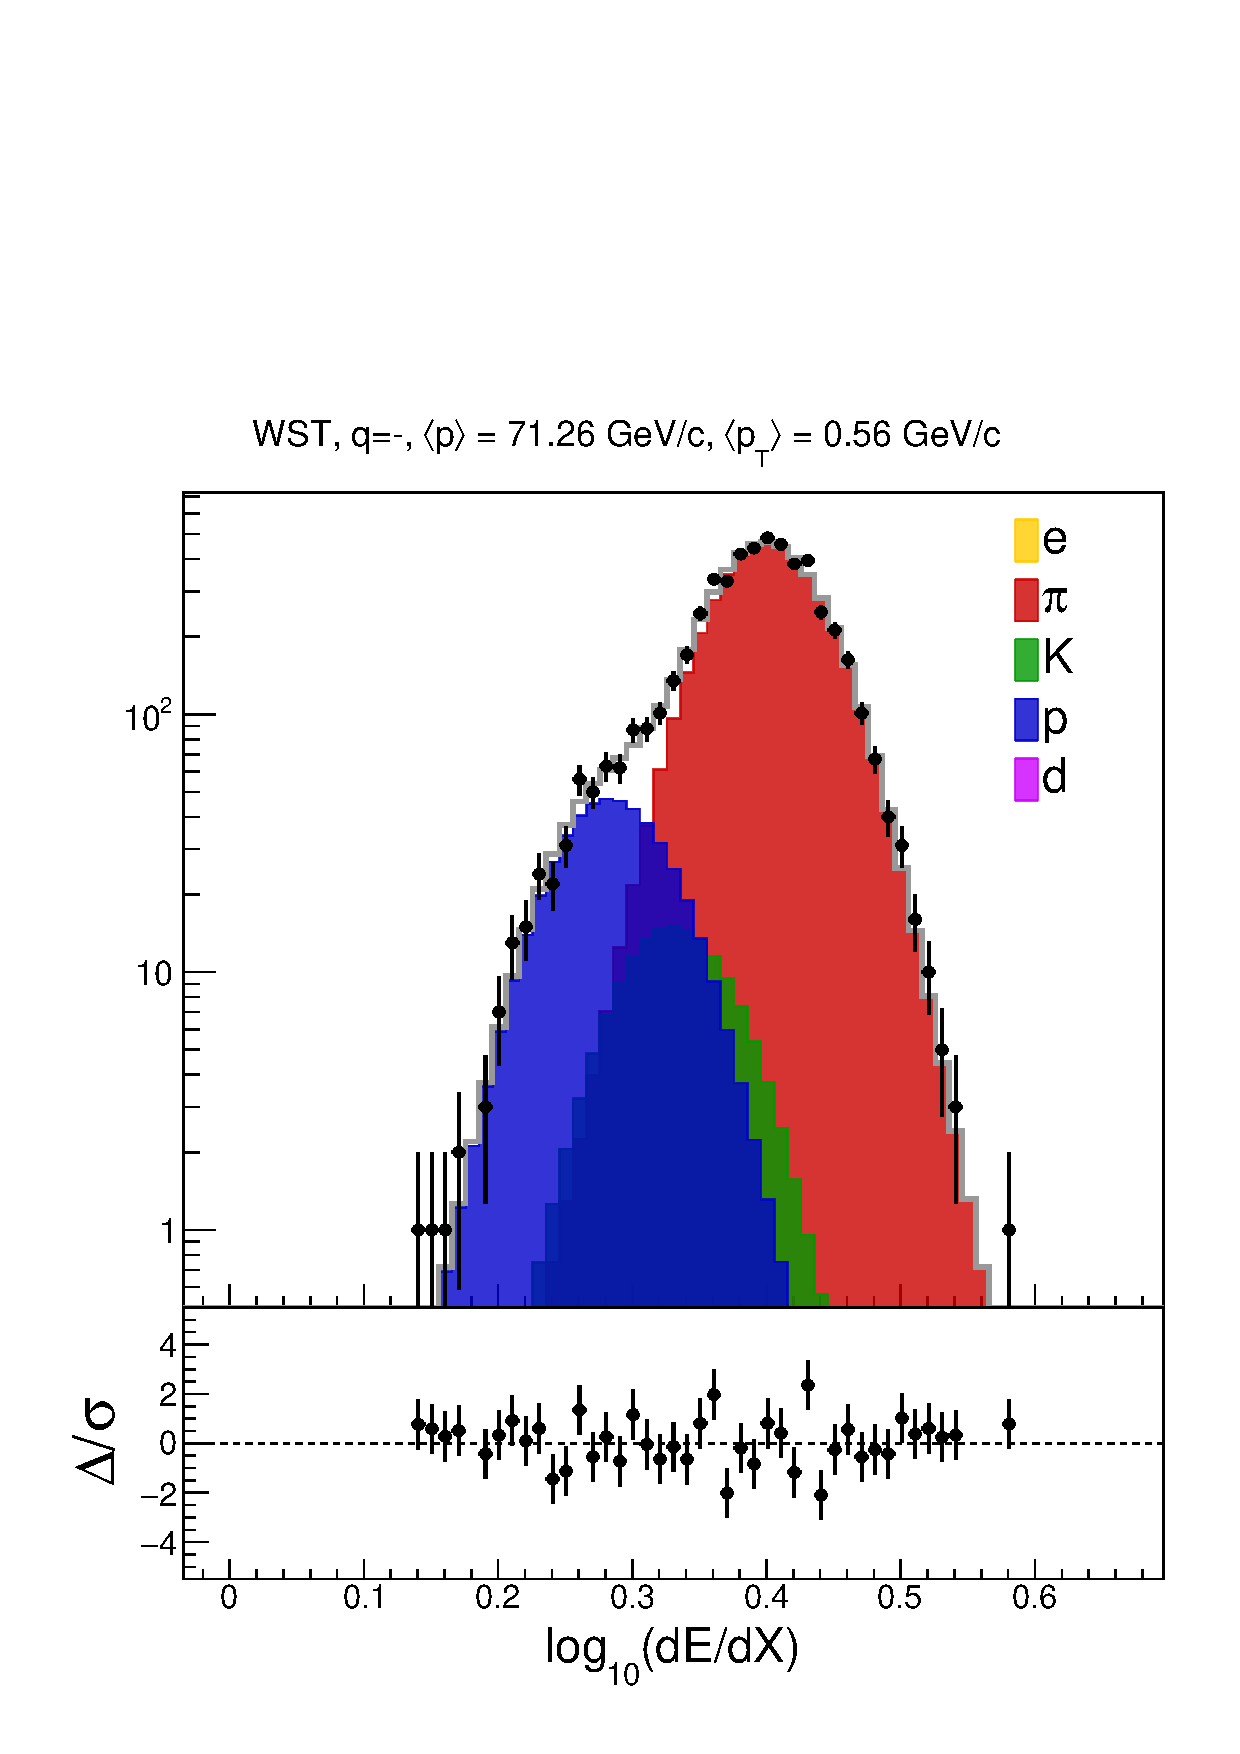
\includegraphics[clip, rviewport=0 0 1 1,width=0.4\textwidth]{dedx/dist_350_v1_c0_x29_y5}
  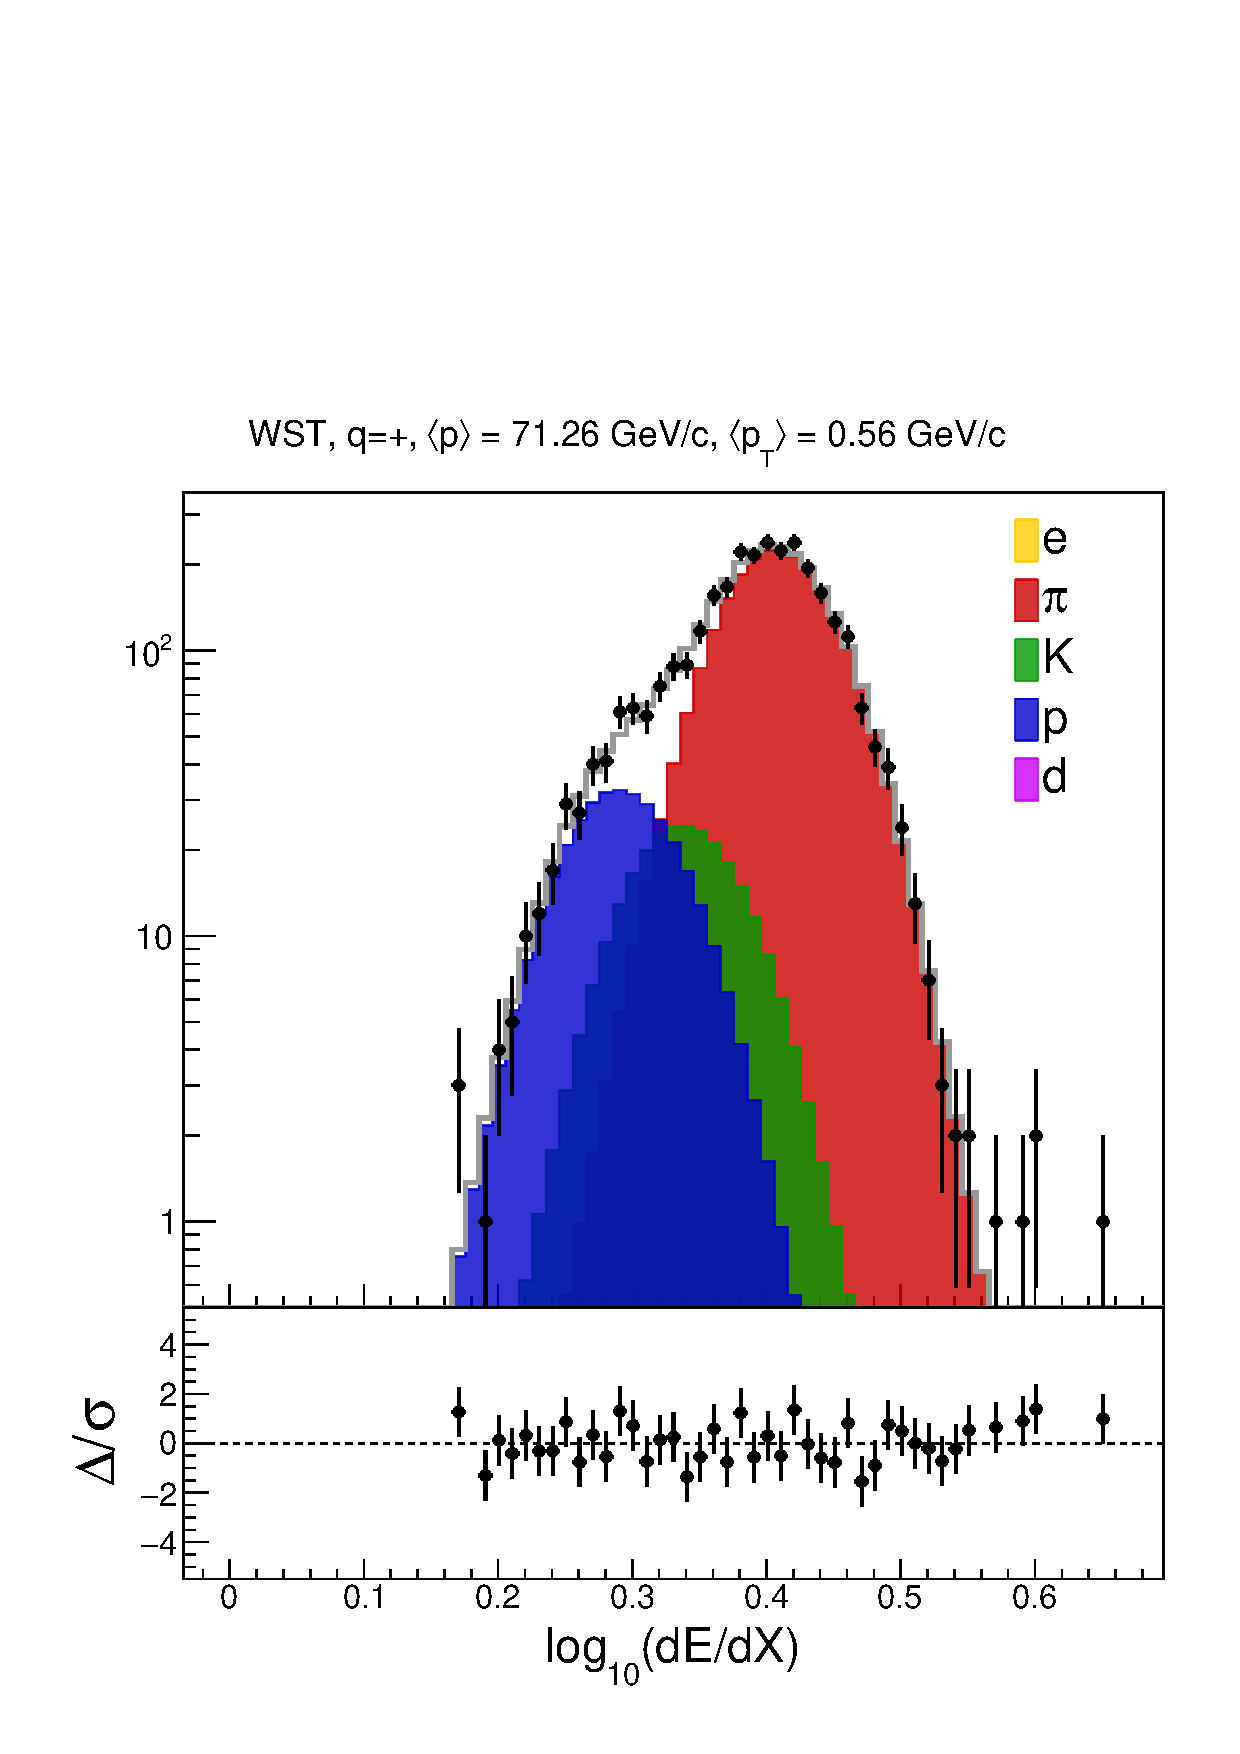
\includegraphics[clip, rviewport=0 0 1 1,width=0.4\textwidth]{dedx/dist_350_v1_c1_x29_y5}
  
  \caption{Examples of the fitted \dedx distributions from the 350 \GeVc dataset.}
  \label{fig:hadron:dedx:fit:dist350}
\end{figure}

%%%%%%%%%% CAL %%%%%%%%%%%%%%
\begin{figure}
  \centering
  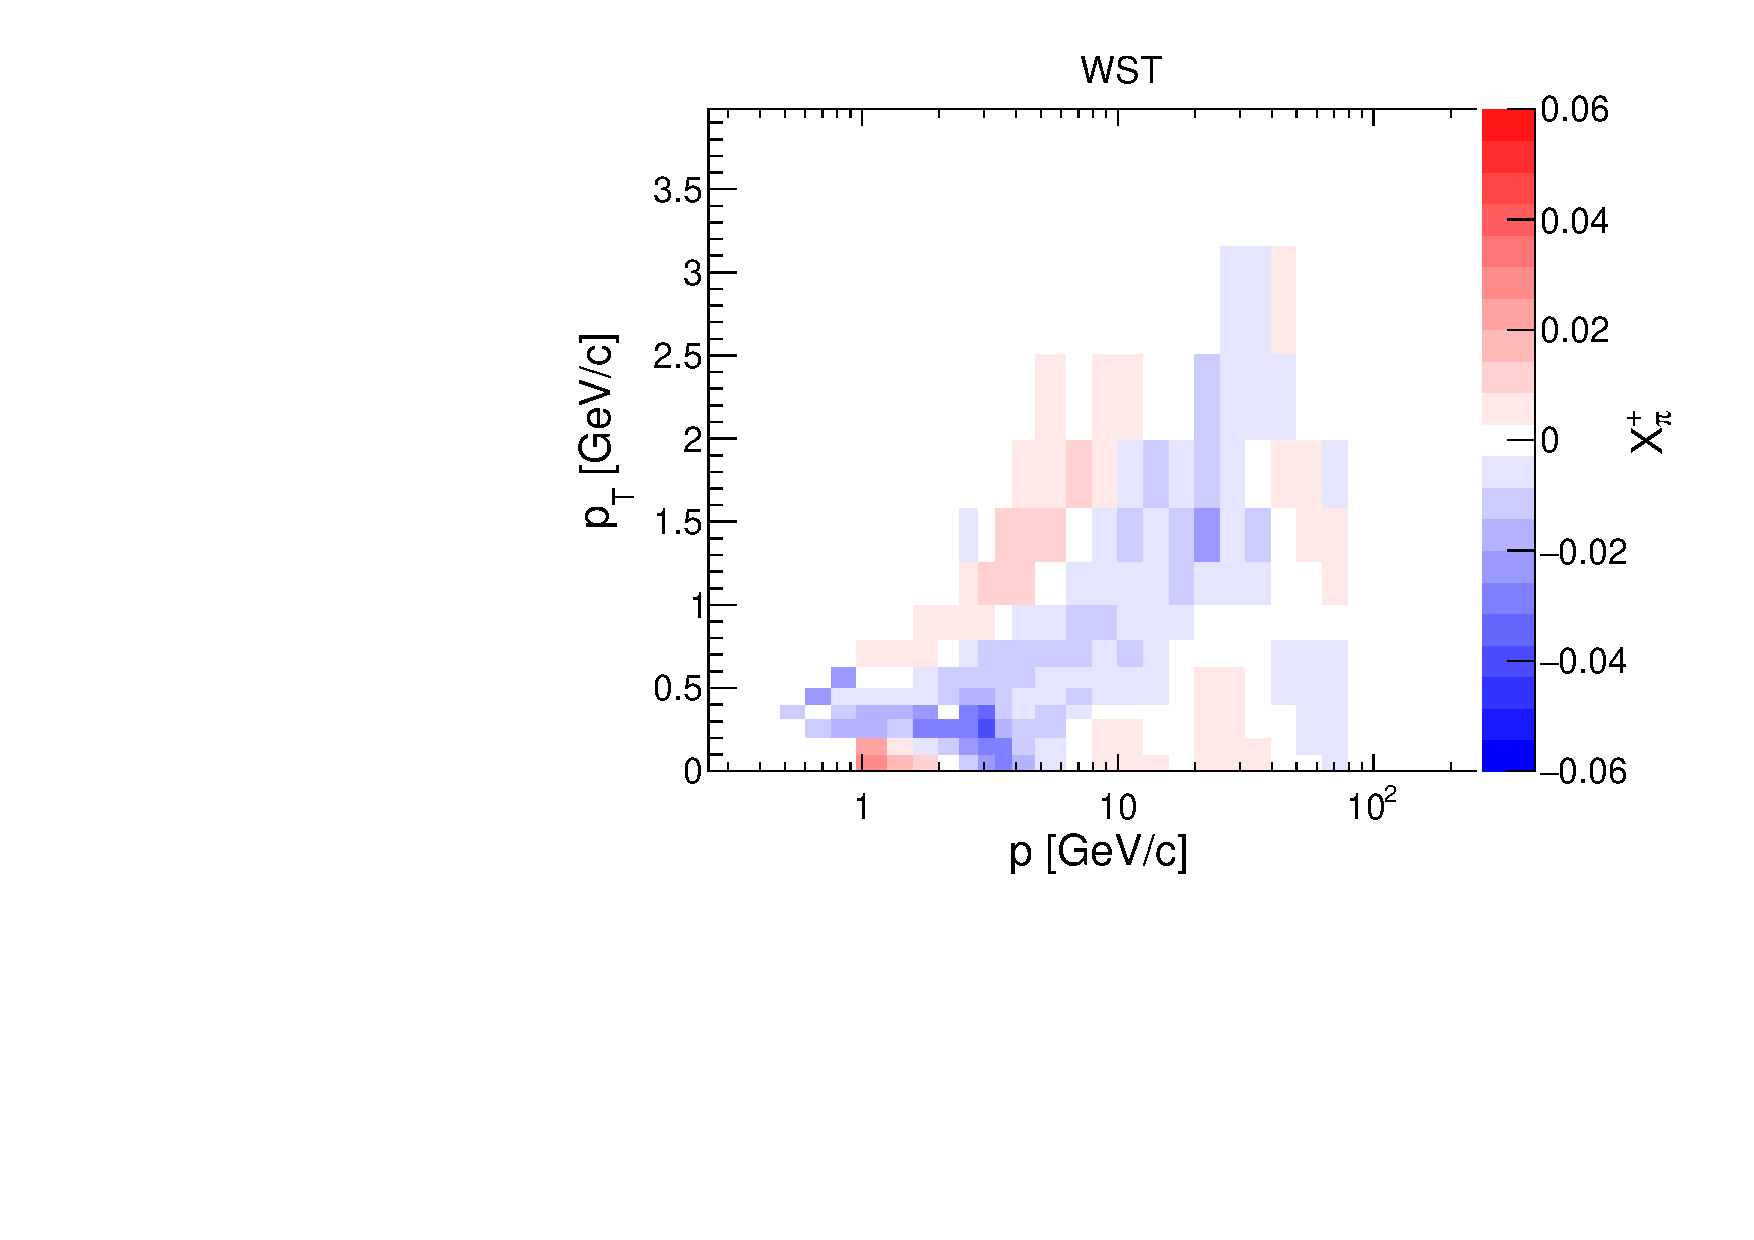
\includegraphics[clip, rviewport=0 0 1 0.94,width=0.4\textwidth]{dedx/model_158_v1_m0}
  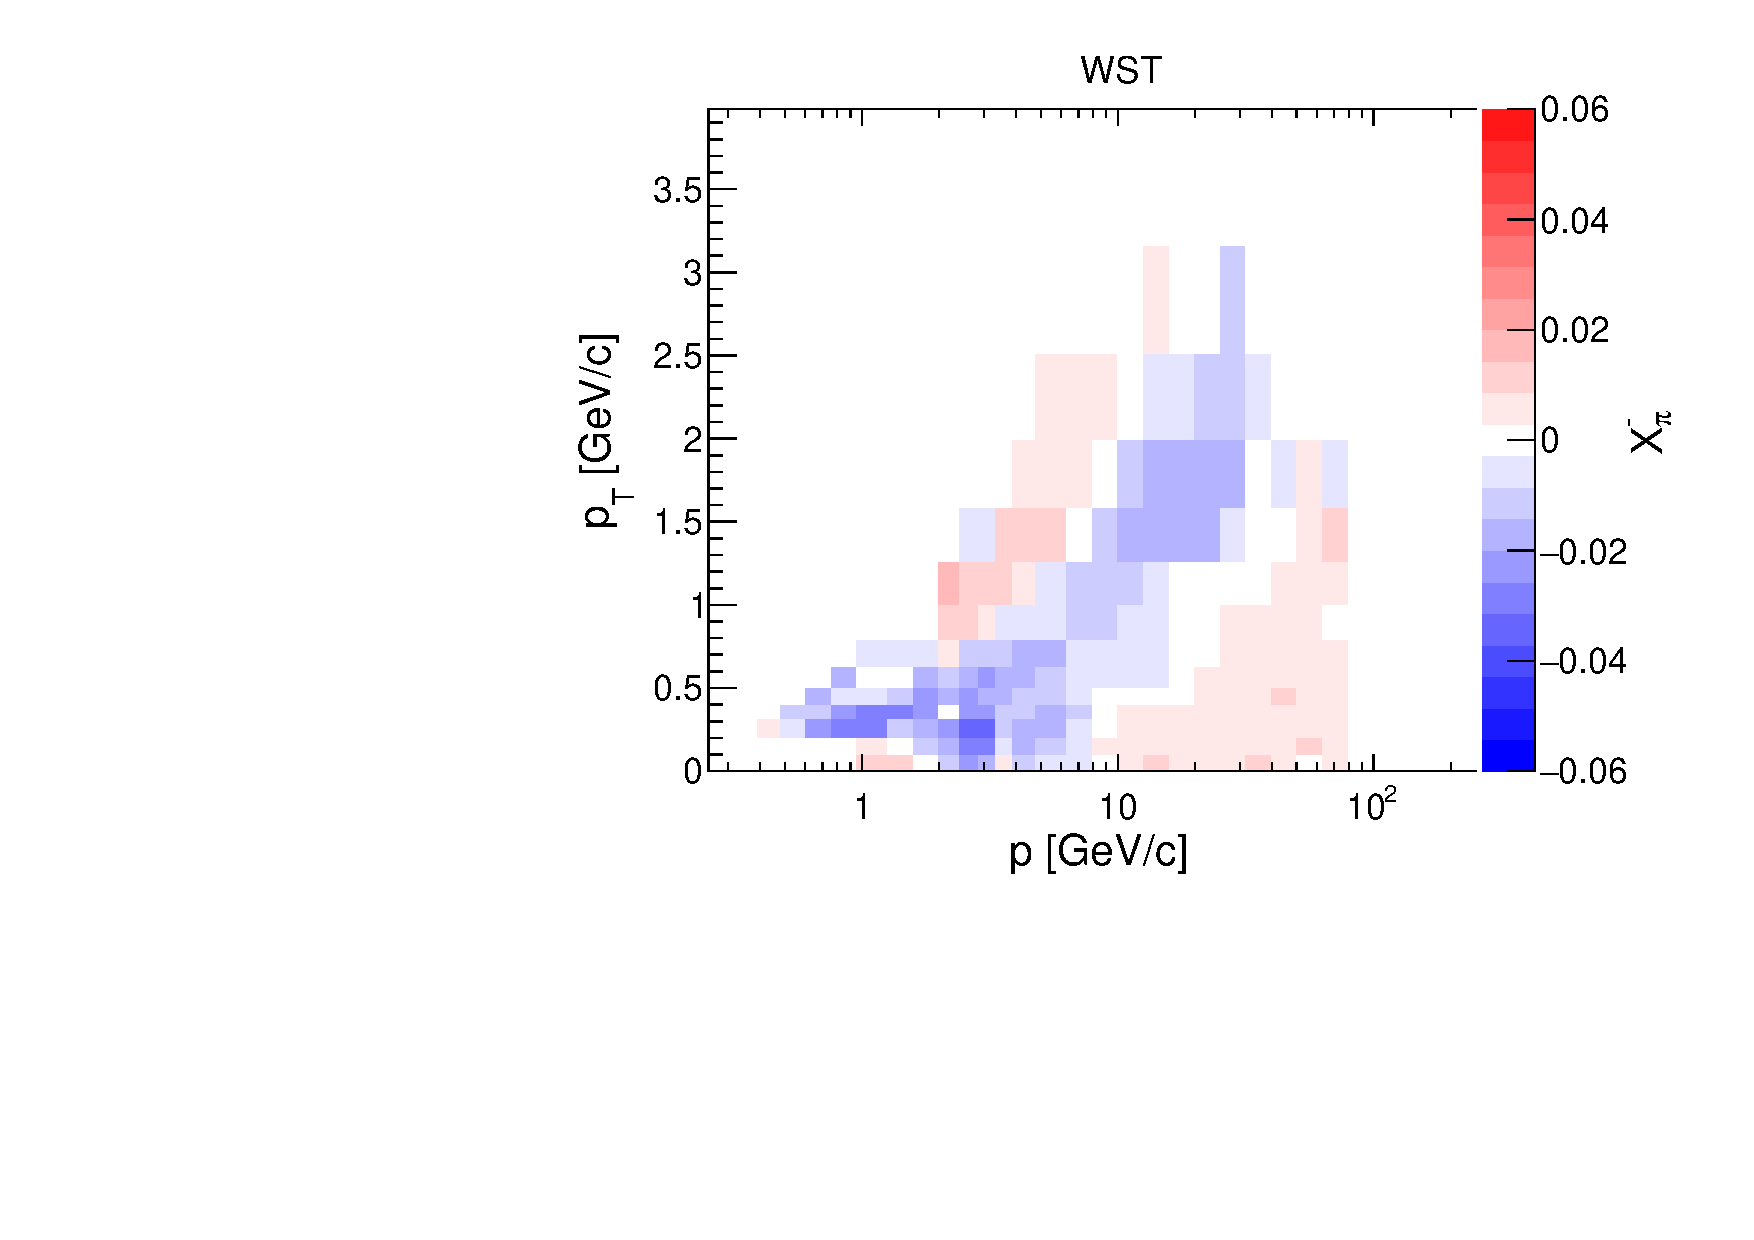
\includegraphics[clip, rviewport=0 0 1 0.94,width=0.4\textwidth]{dedx/model_158_v1_m1}

  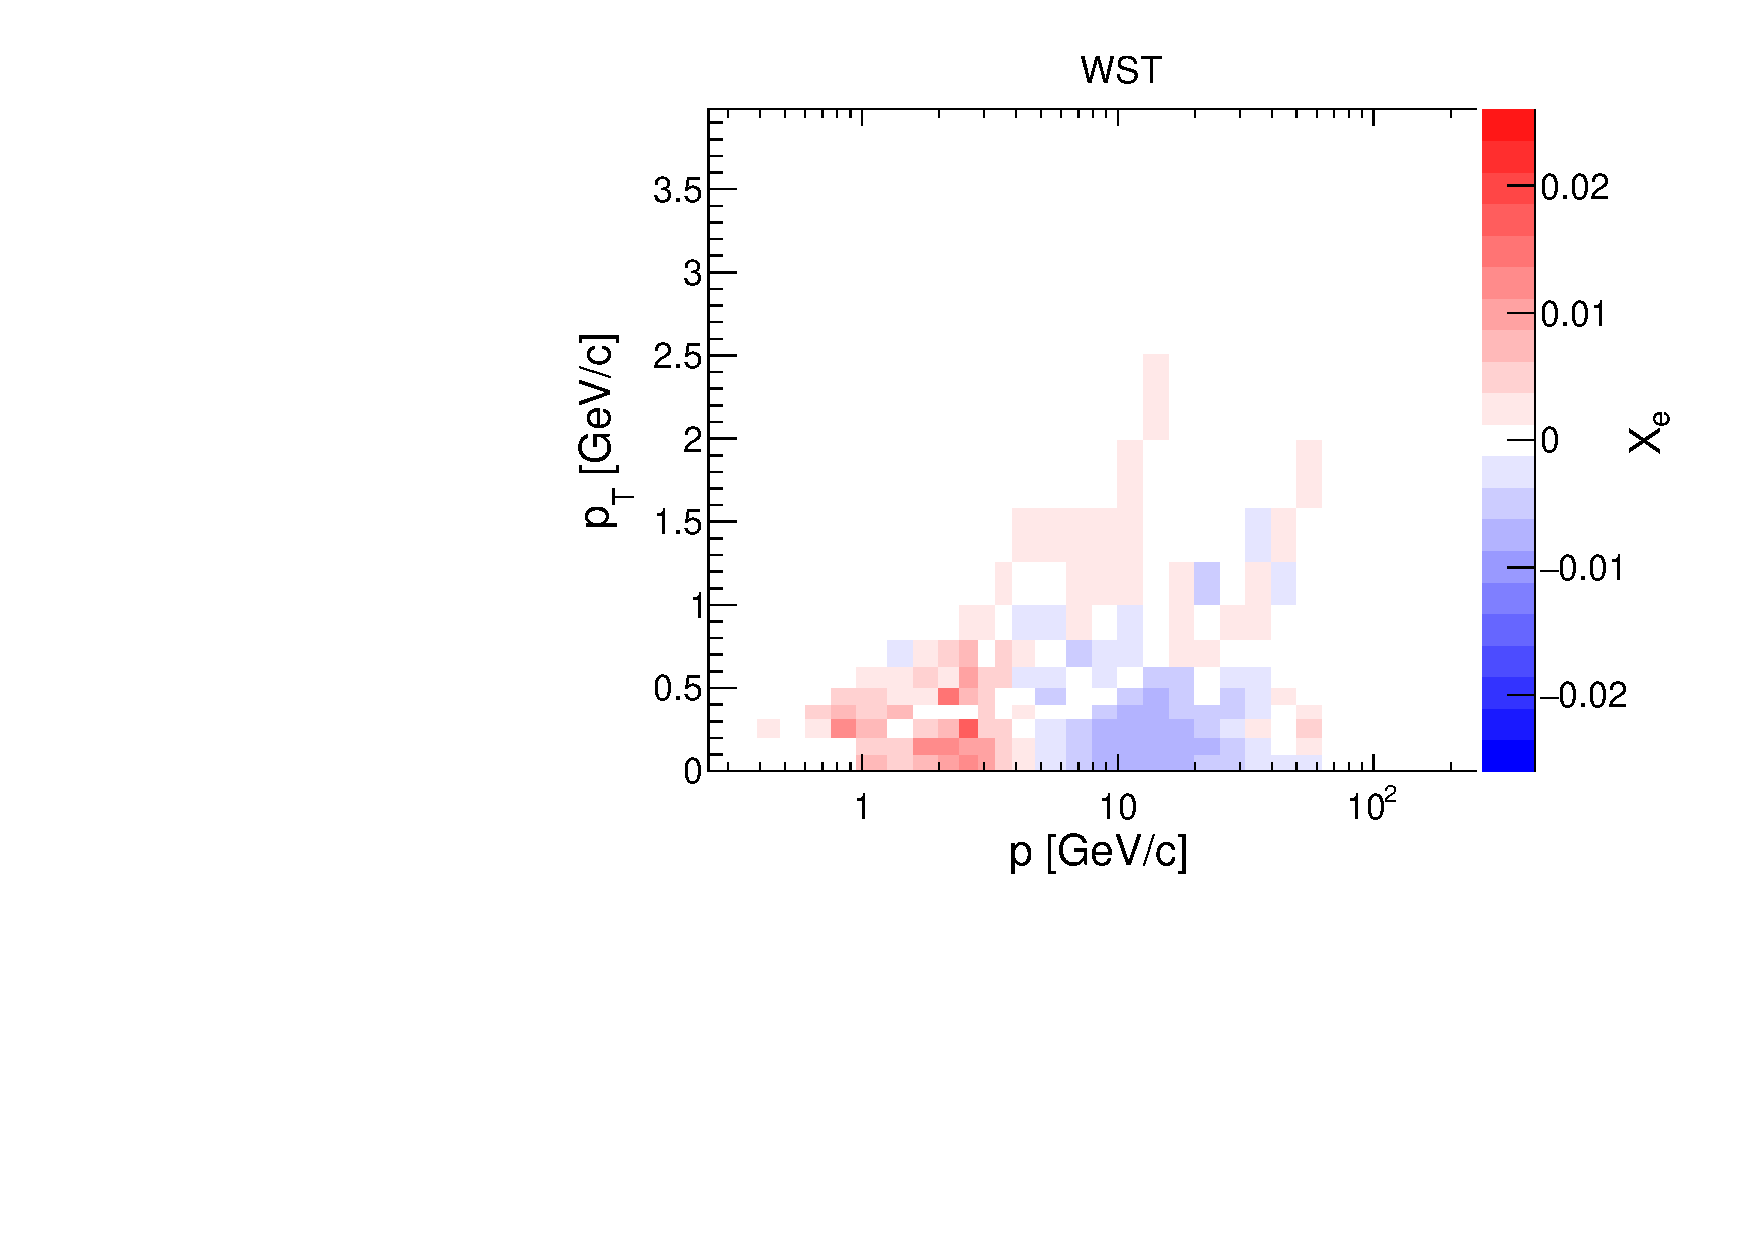
\includegraphics[clip, rviewport=0 0 1 0.94,width=0.4\textwidth]{dedx/model_158_v1_m2}
  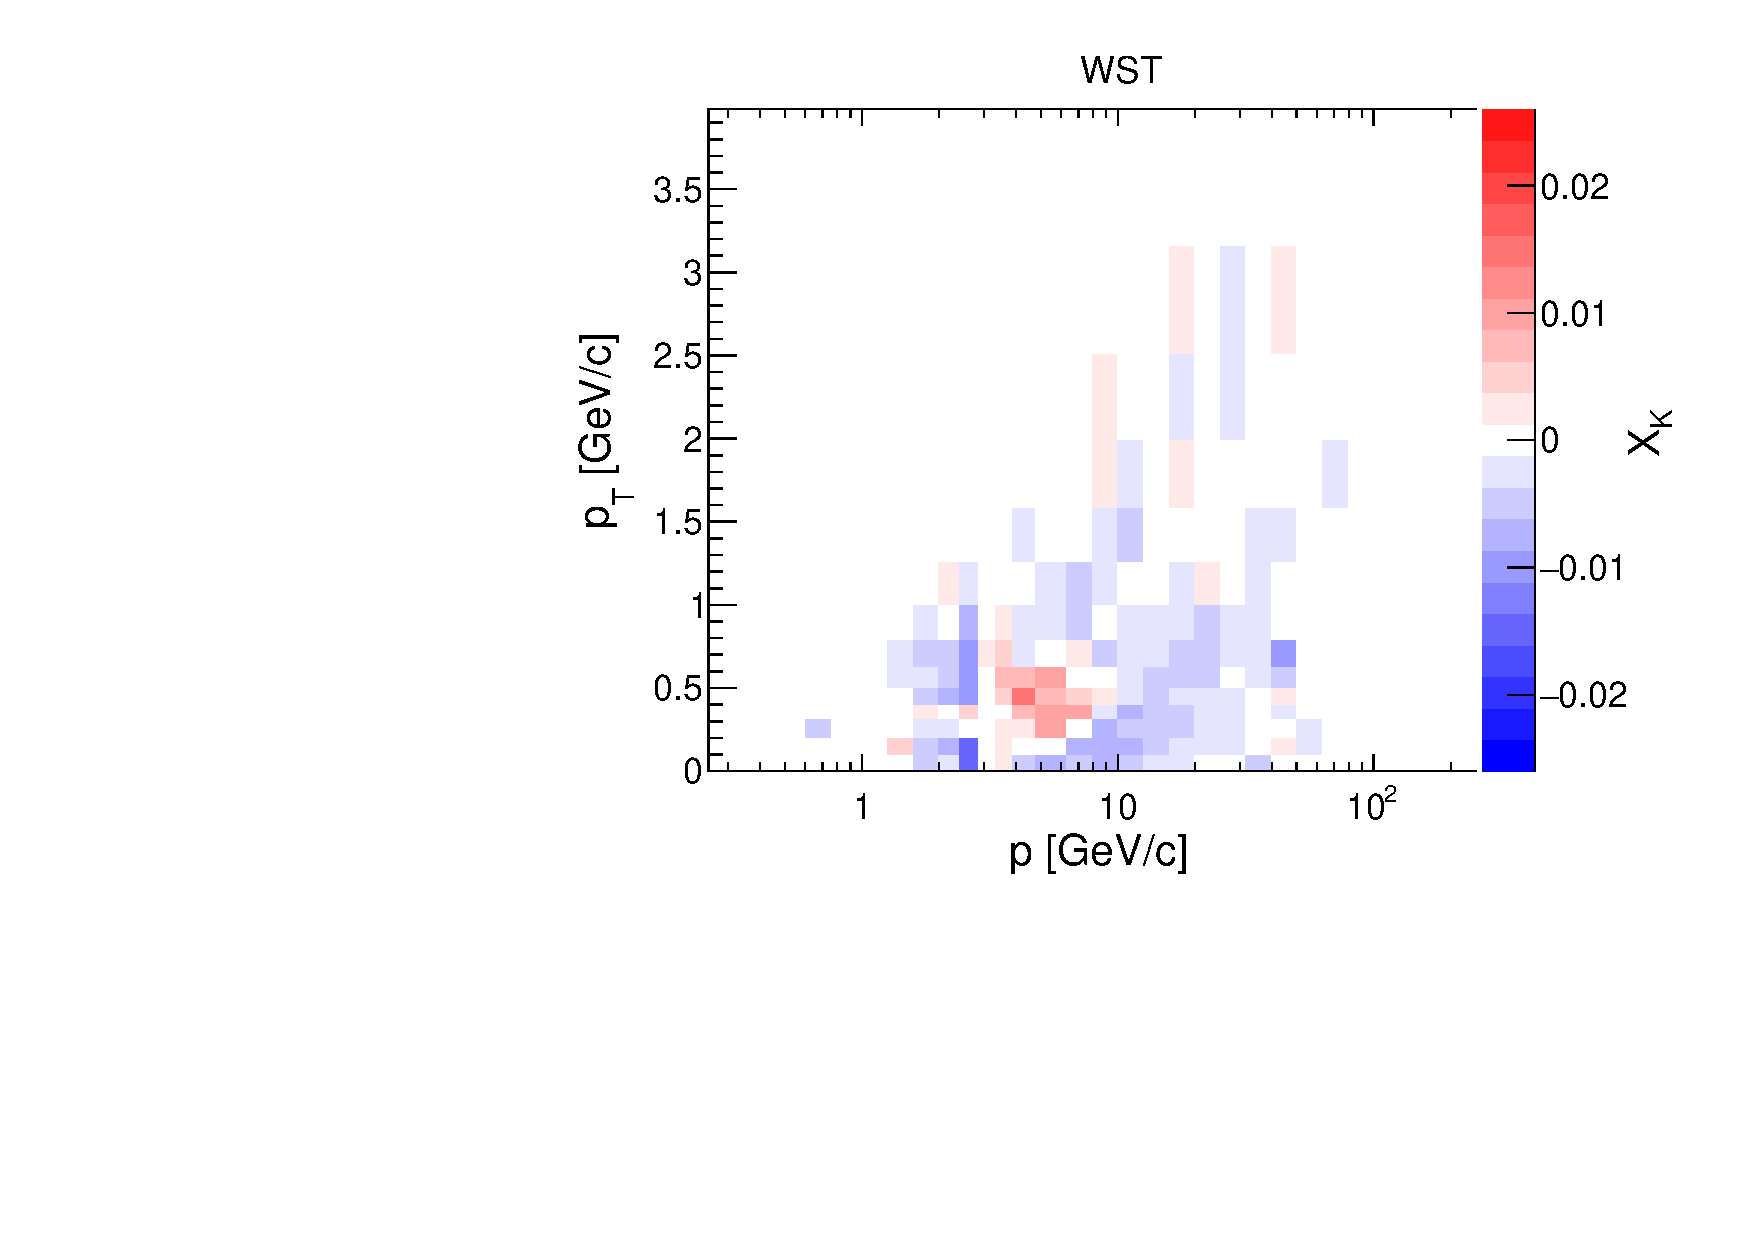
\includegraphics[clip, rviewport=0 0 1 0.94,width=0.4\textwidth]{dedx/model_158_v1_m3}

  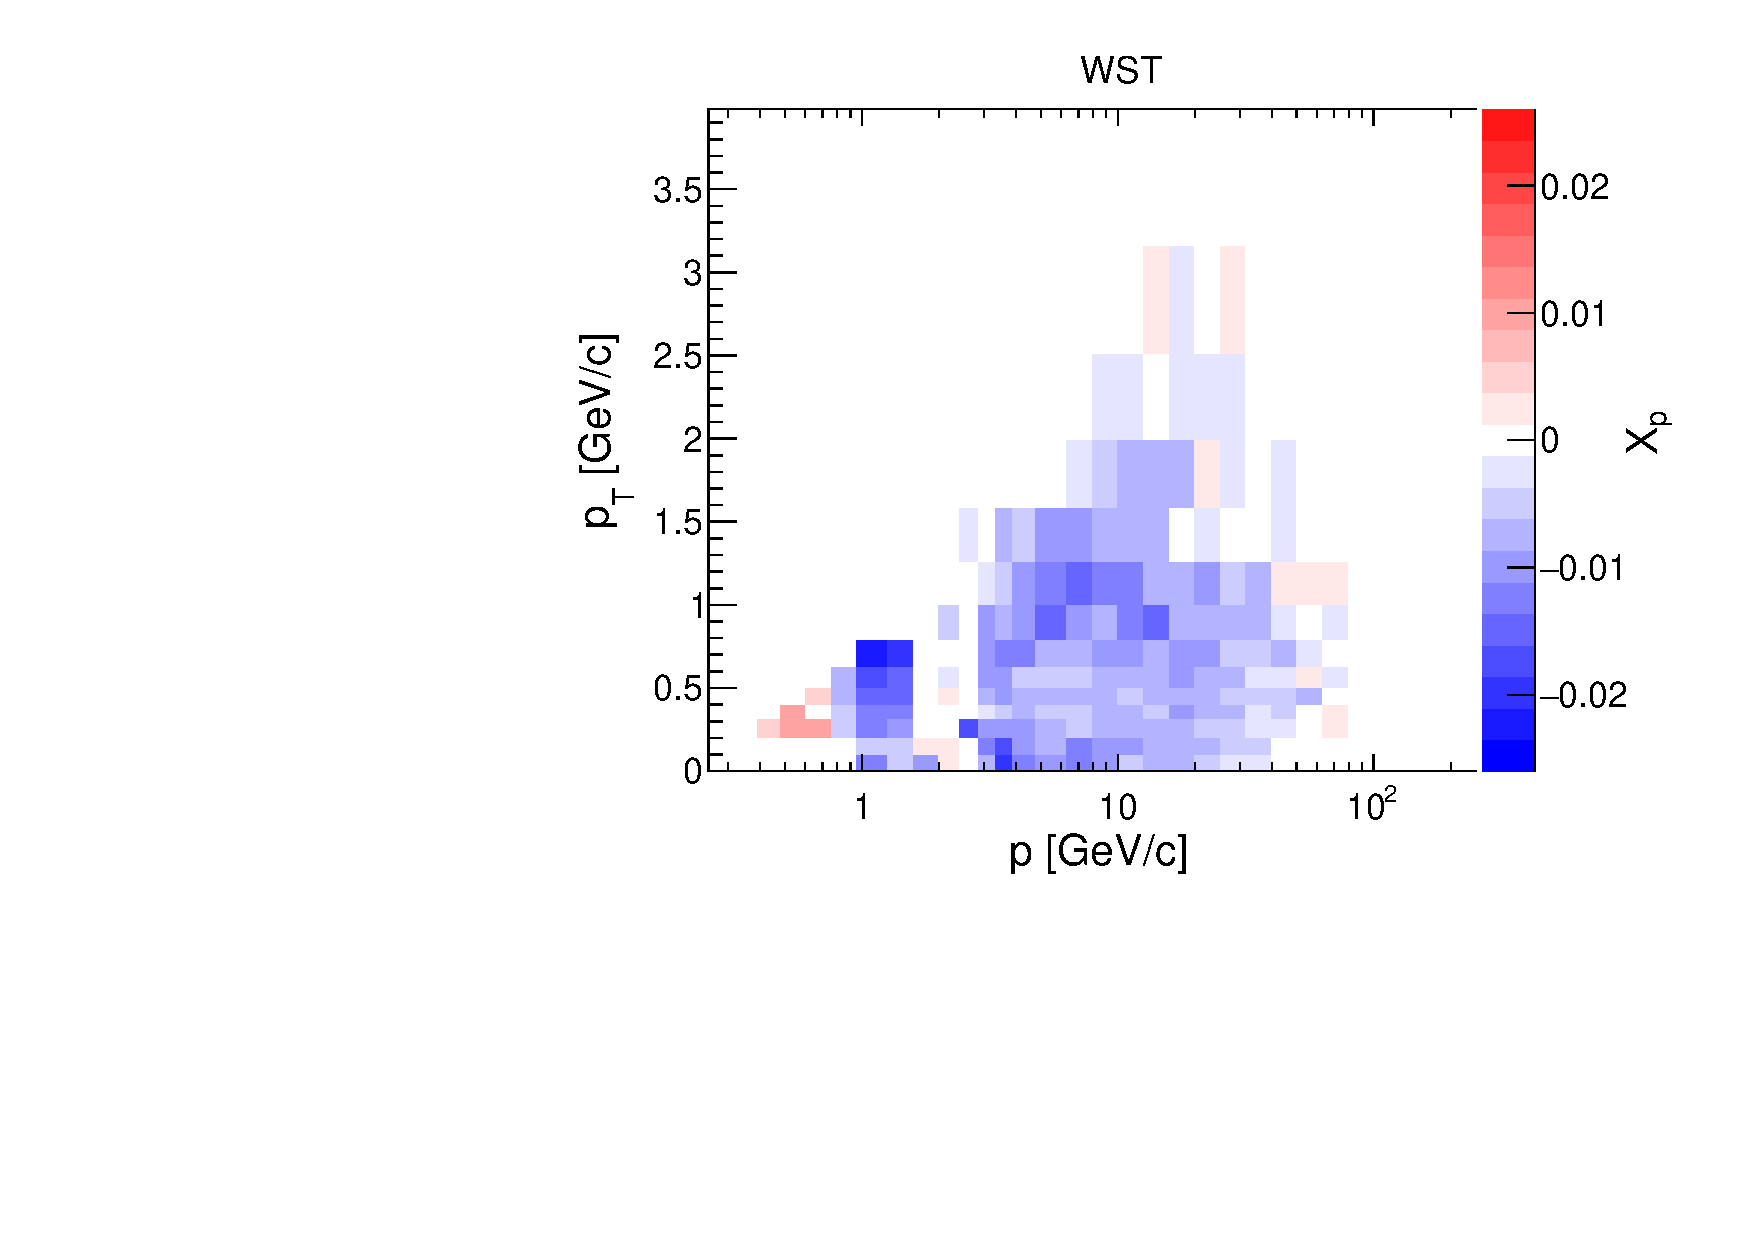
\includegraphics[clip, rviewport=0 0 1 0.94,width=0.4\textwidth]{dedx/model_158_v1_m4}
  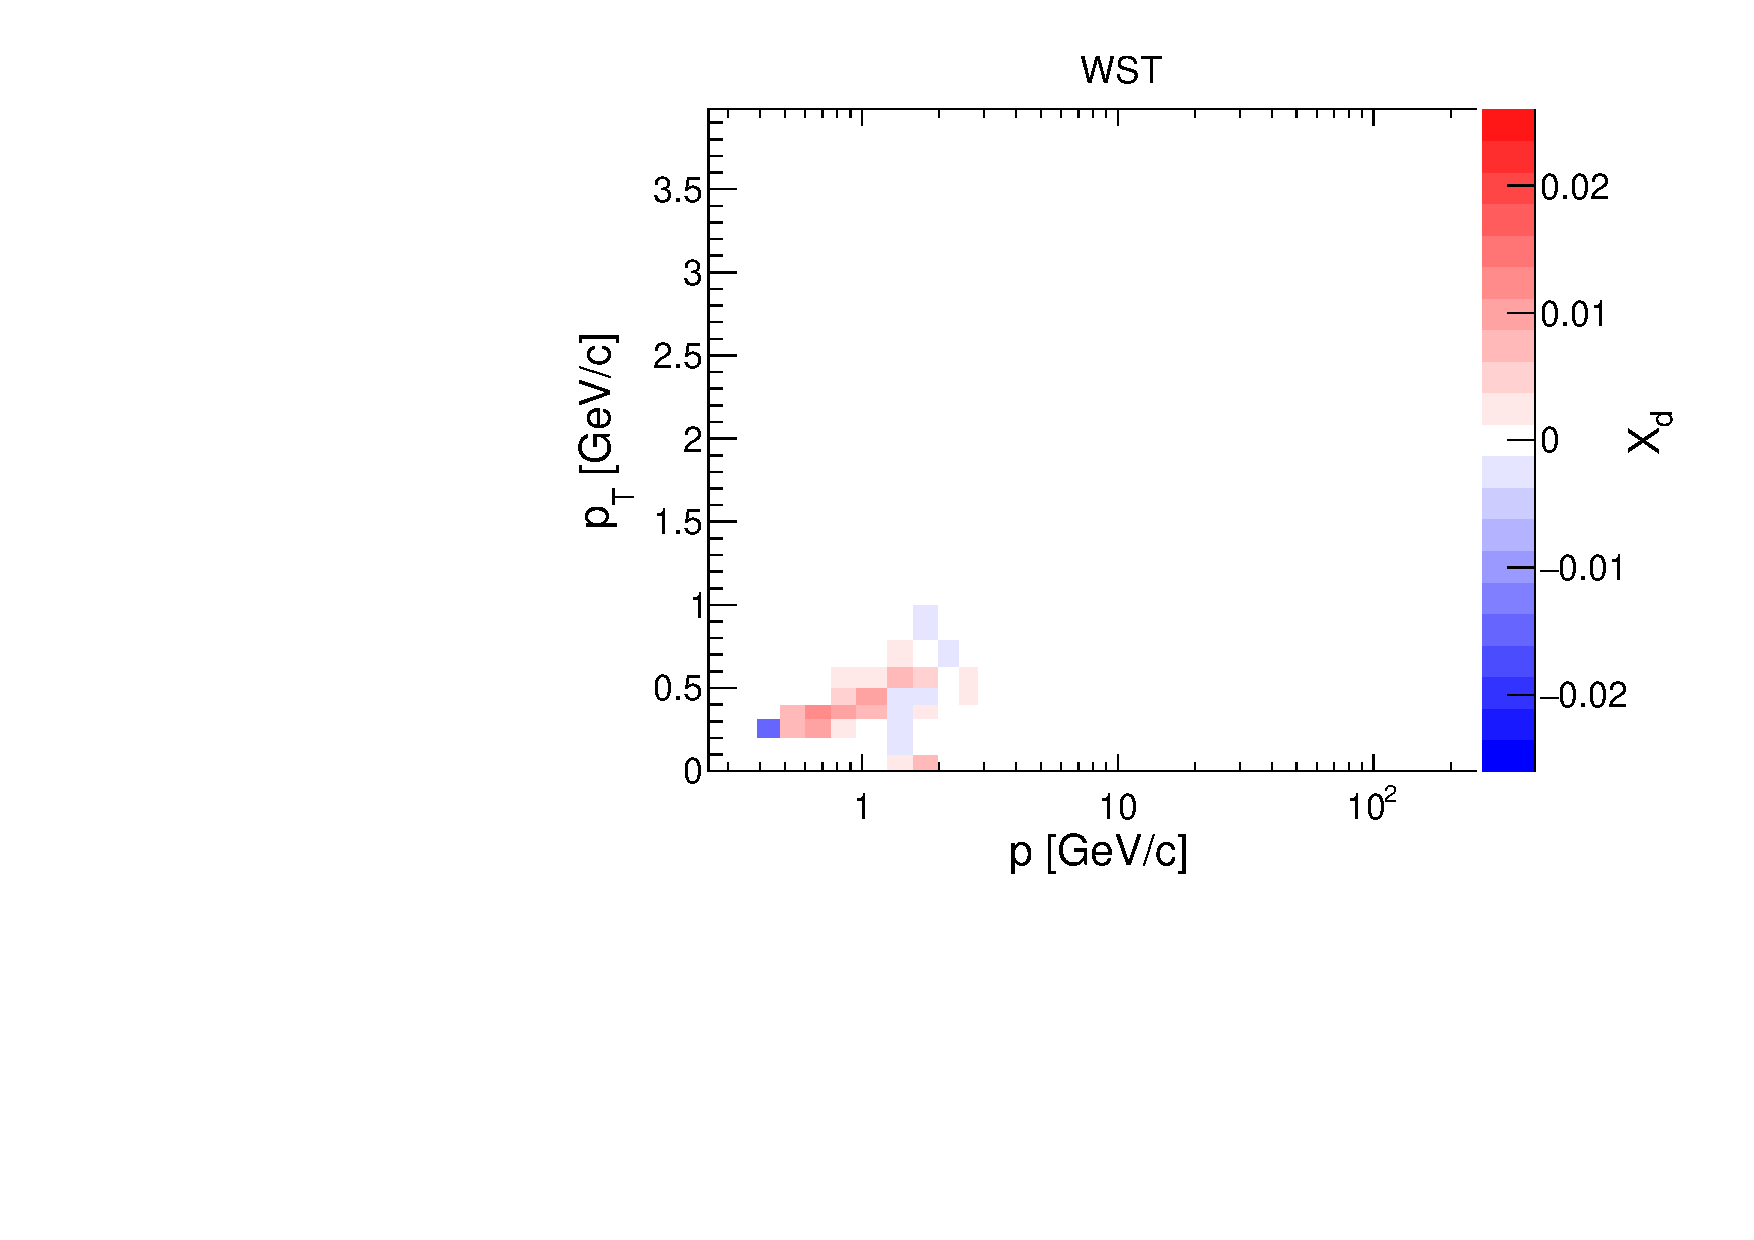
\includegraphics[clip, rviewport=0 0 1 0.94,width=0.4\textwidth]{dedx/model_158_v1_m5}
  \caption{Calibration constants obtained from the fit of the WST dataset at 158 \GeVc.}
  \label{fig:hadron:dedx:fit:cal158w}
\end{figure}

%%%%%%%%%% CAL %%%%%%%%%%%%%%
\begin{figure}
  \centering
  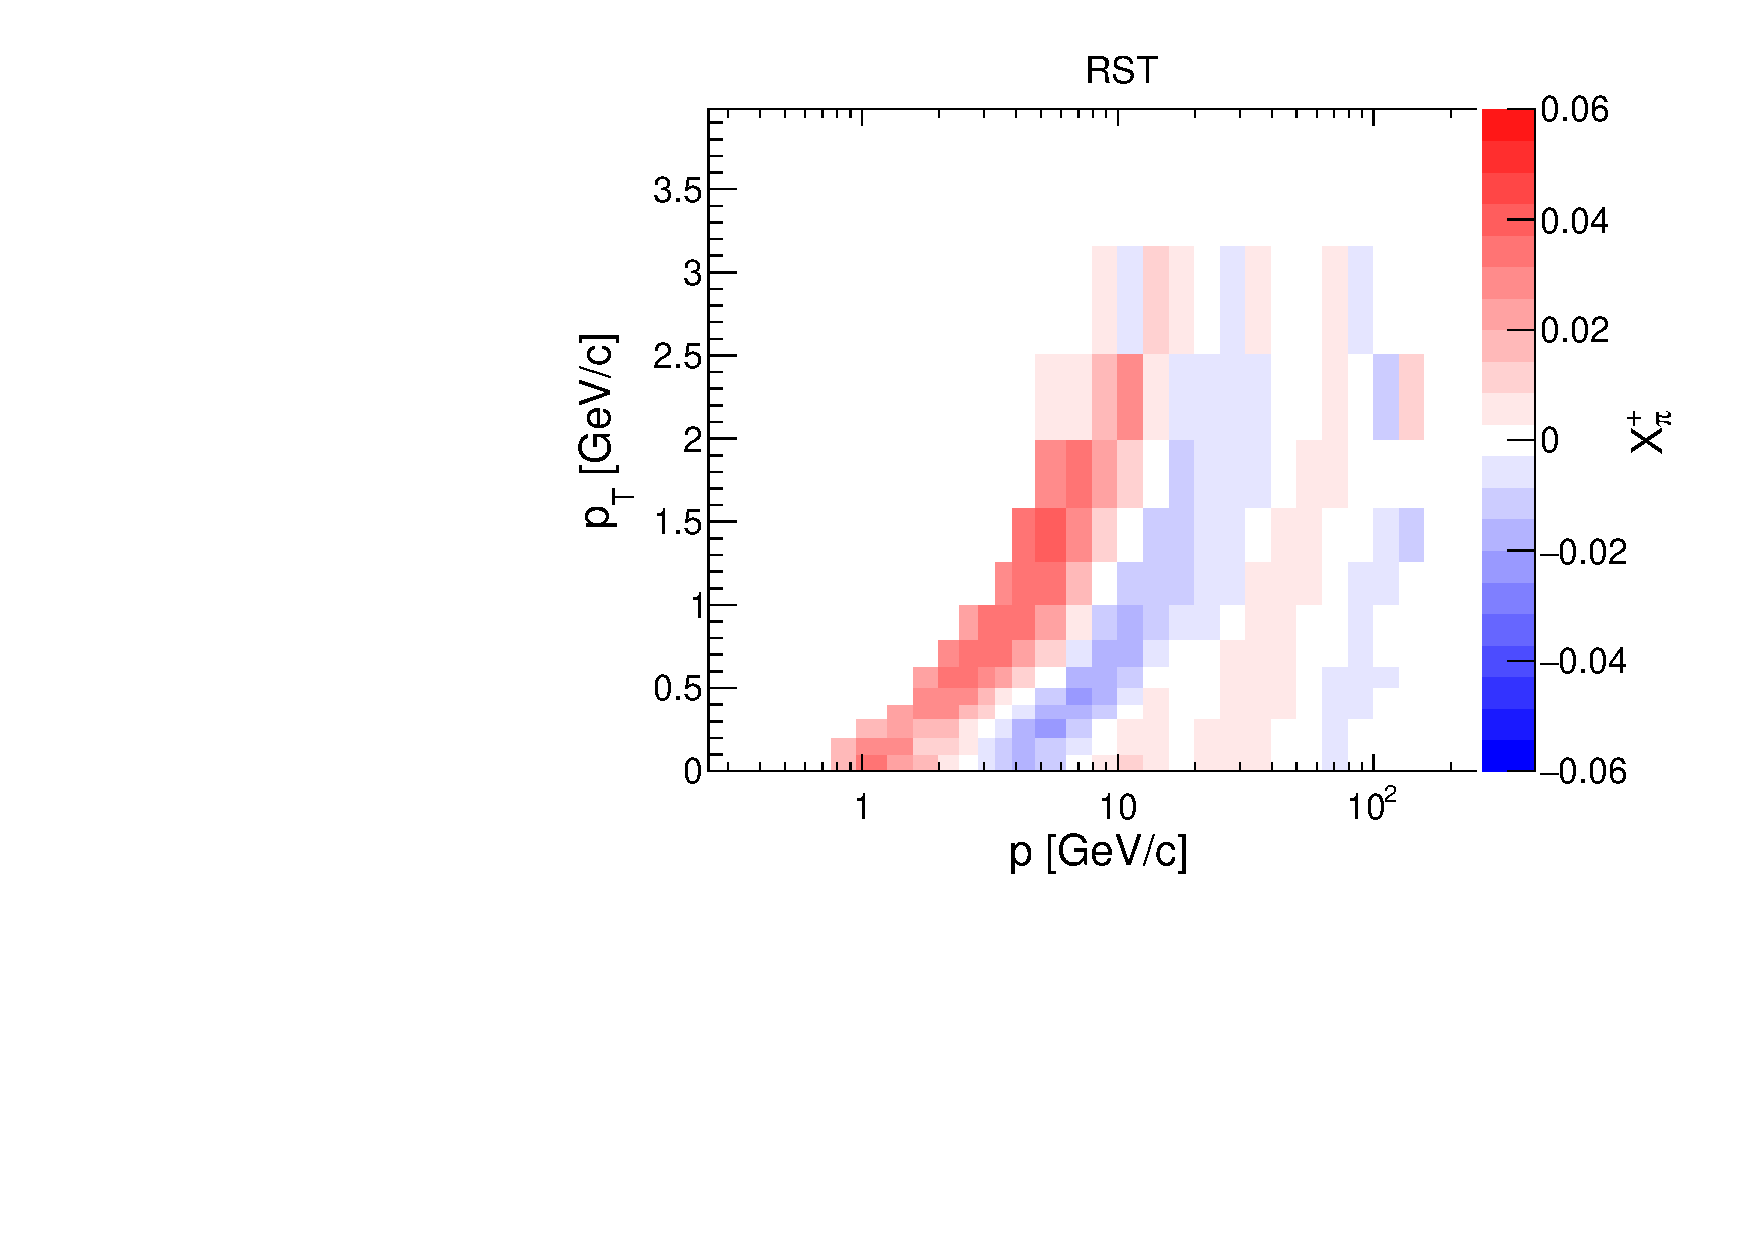
\includegraphics[clip, rviewport=0 0 1 0.94,width=0.4\textwidth]{dedx/model_350_v0_m0}
  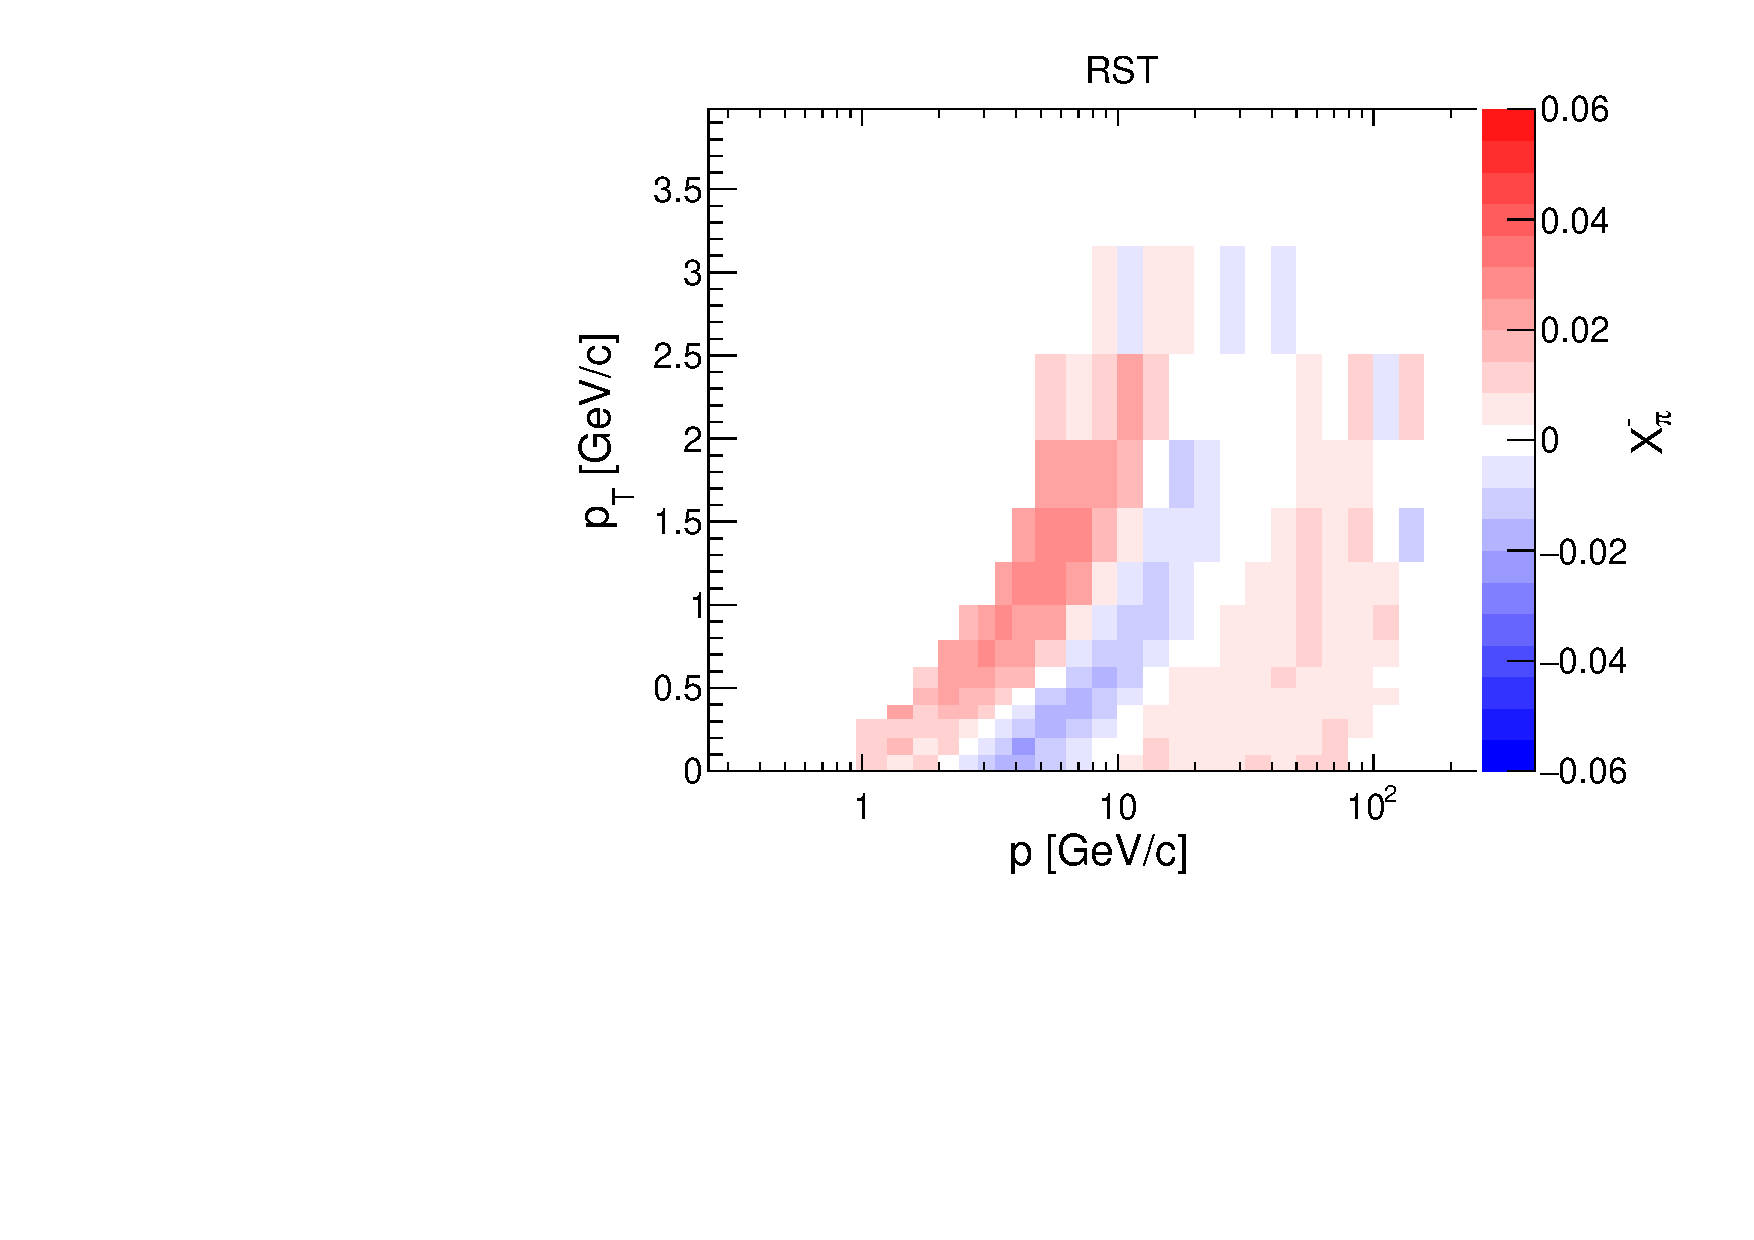
\includegraphics[clip, rviewport=0 0 1 0.94,width=0.4\textwidth]{dedx/model_350_v0_m1}

  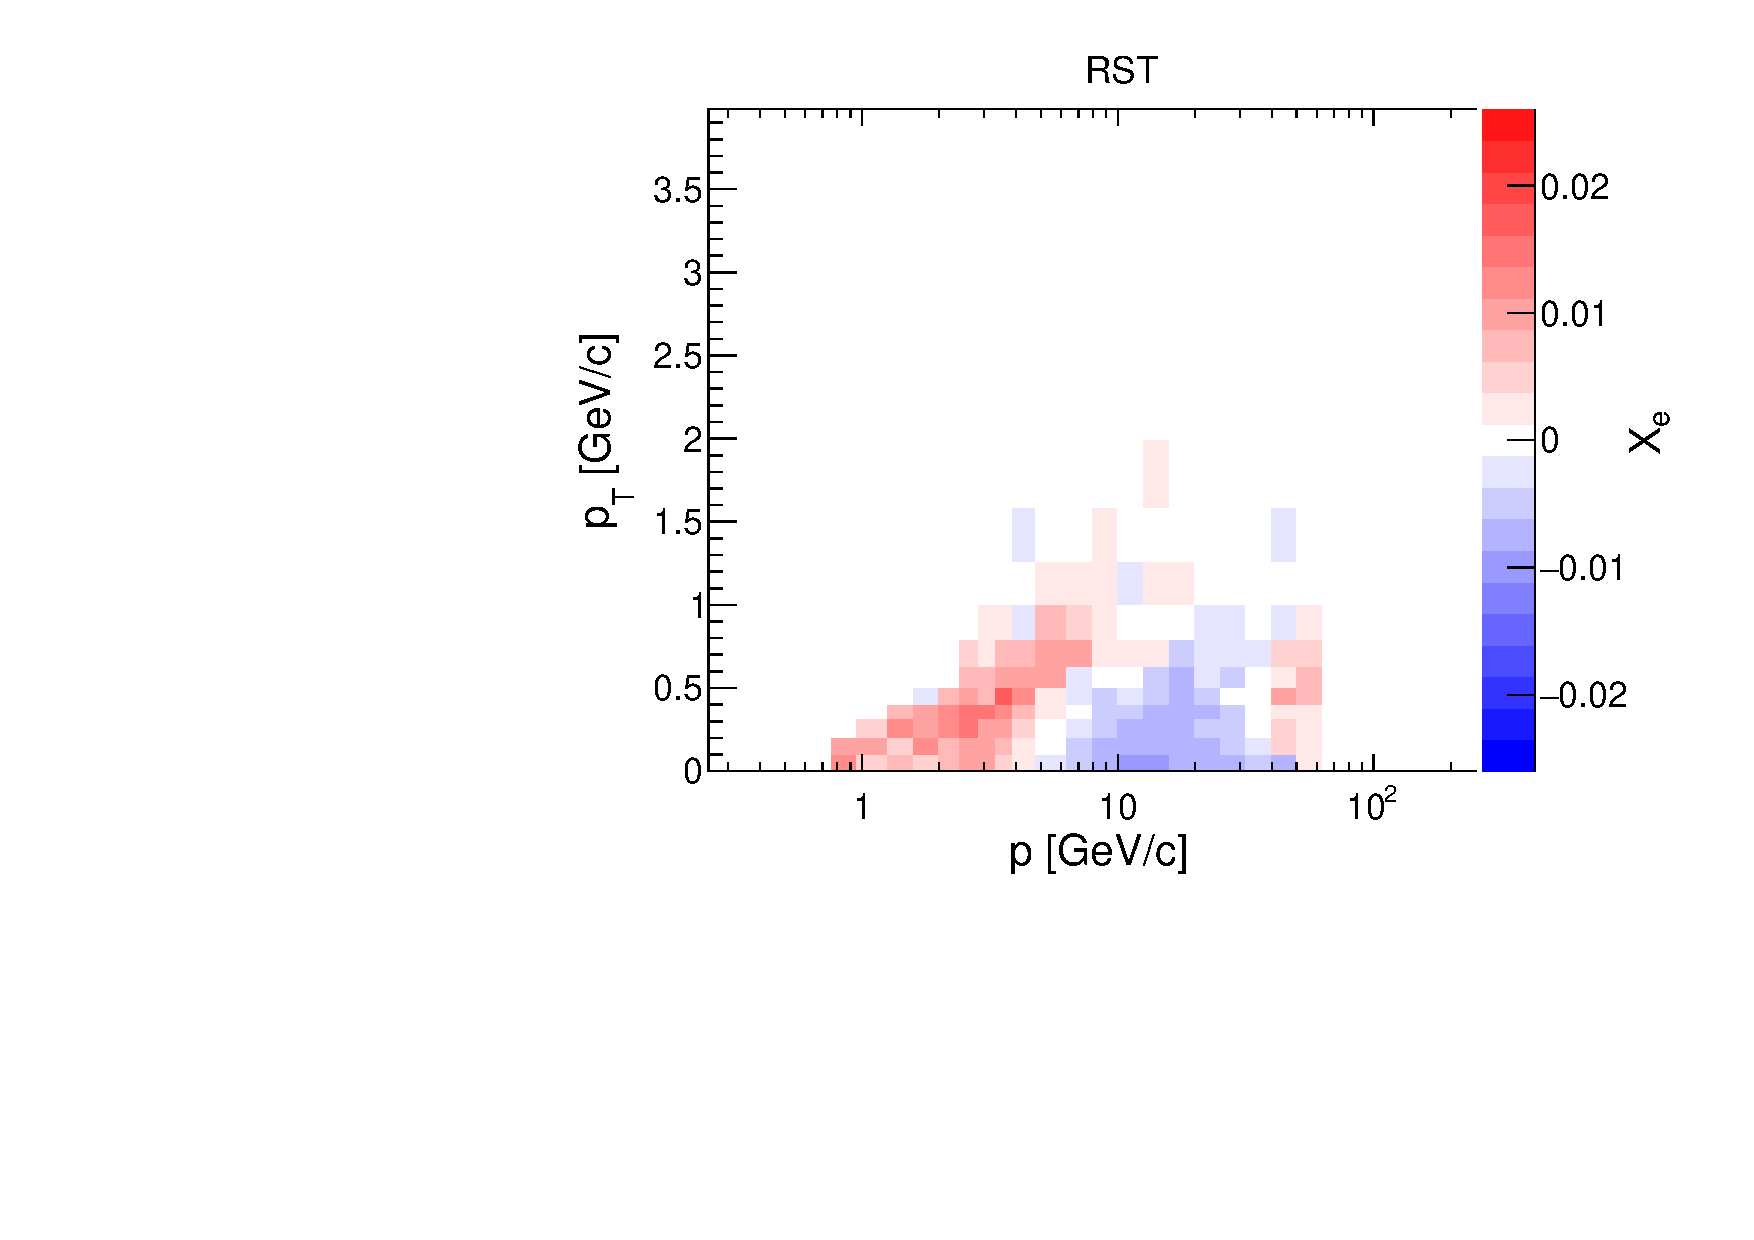
\includegraphics[clip, rviewport=0 0 1 0.94,width=0.4\textwidth]{dedx/model_350_v0_m2}
  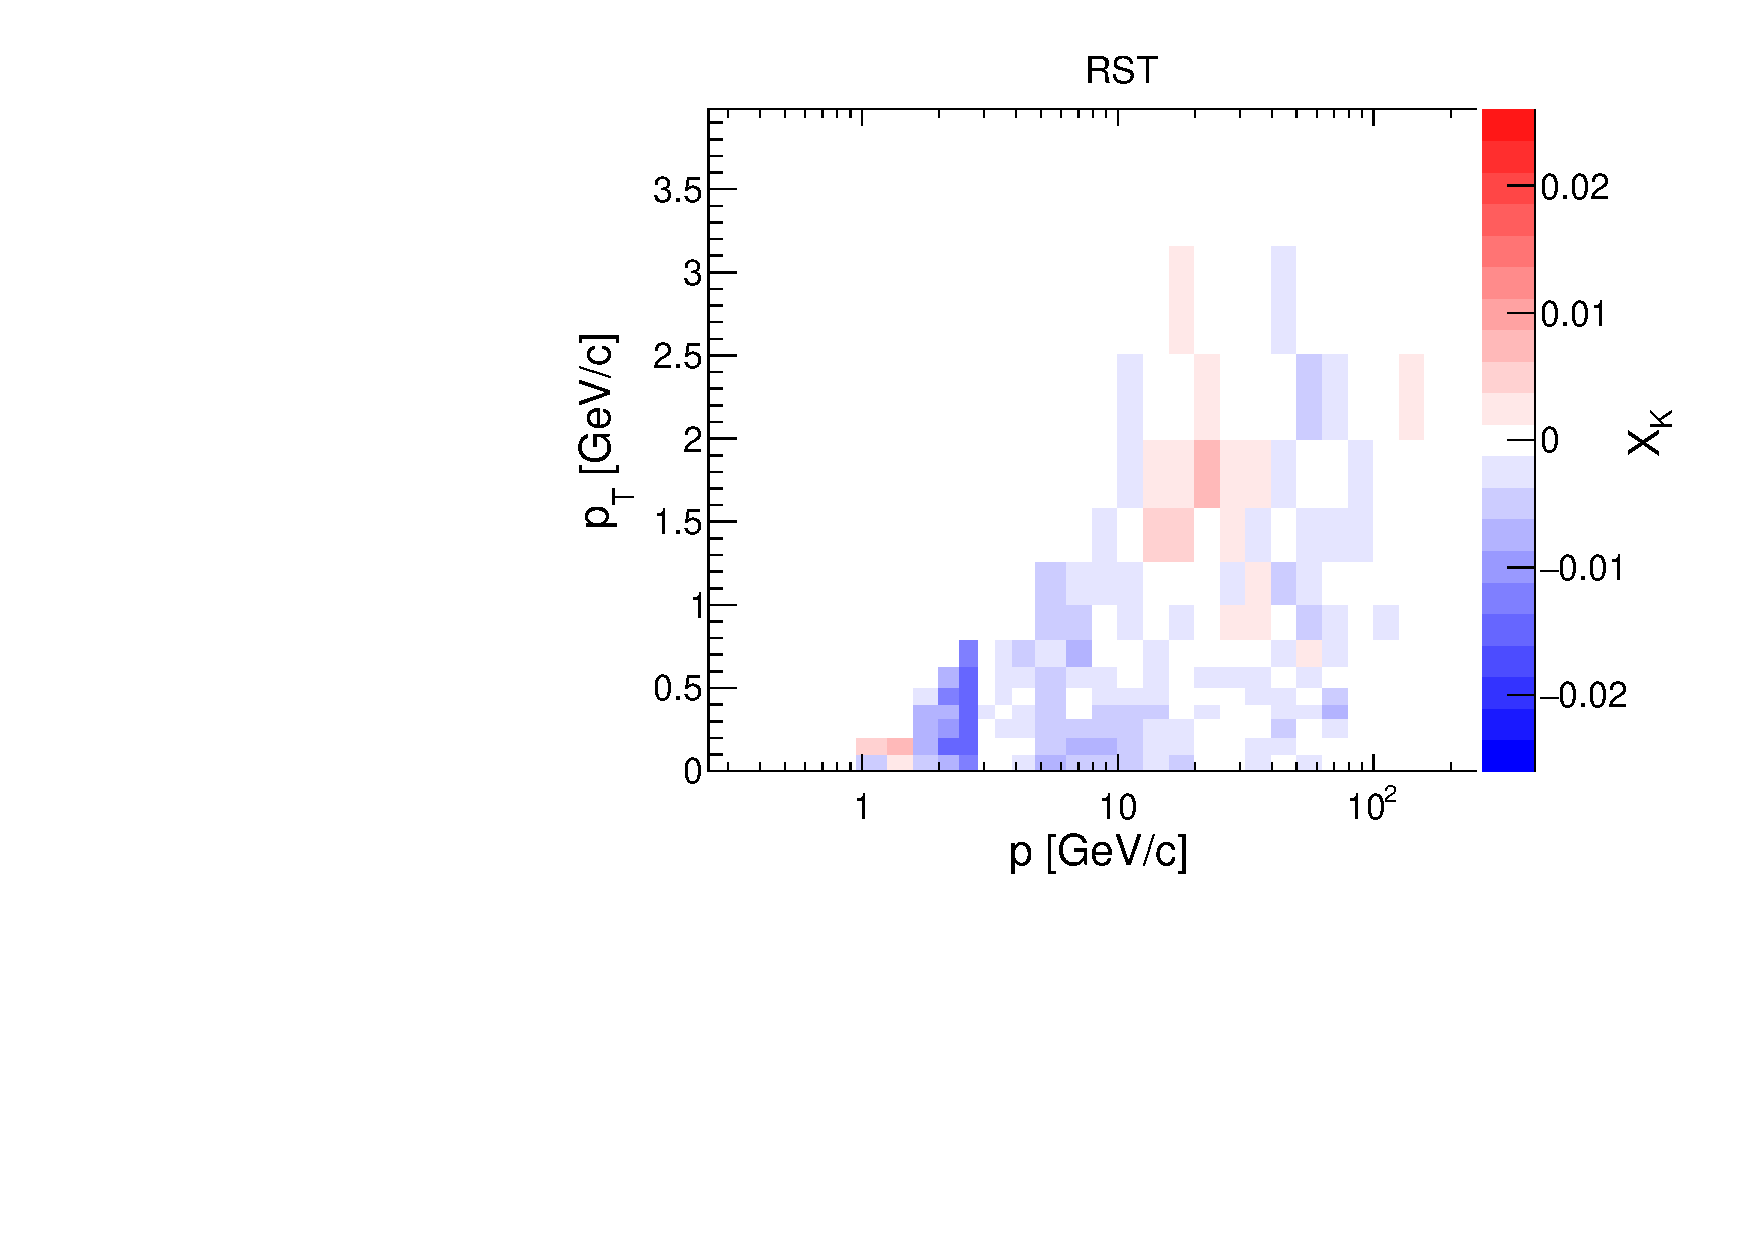
\includegraphics[clip, rviewport=0 0 1 0.94,width=0.4\textwidth]{dedx/model_350_v0_m3}

  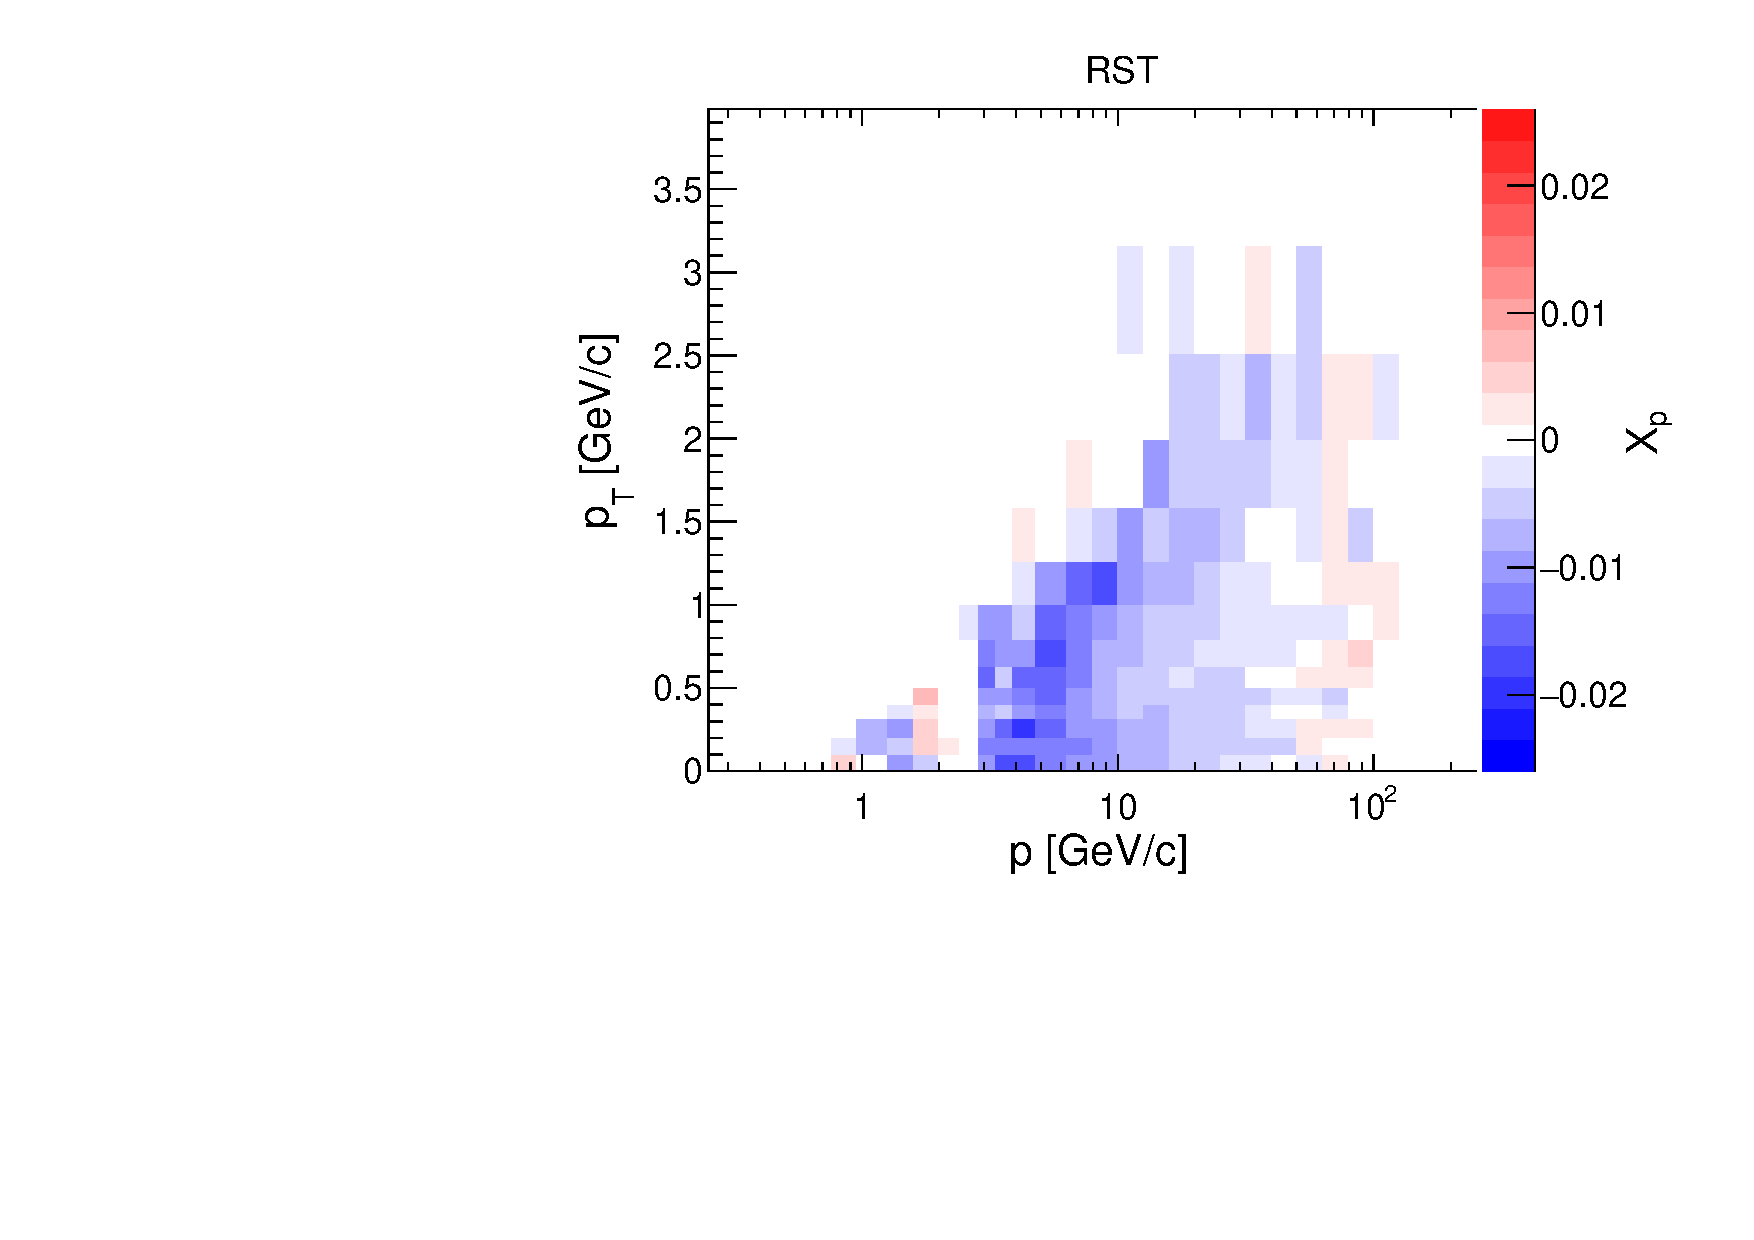
\includegraphics[clip, rviewport=0 0 1 0.94,width=0.4\textwidth]{dedx/model_350_v0_m4}
  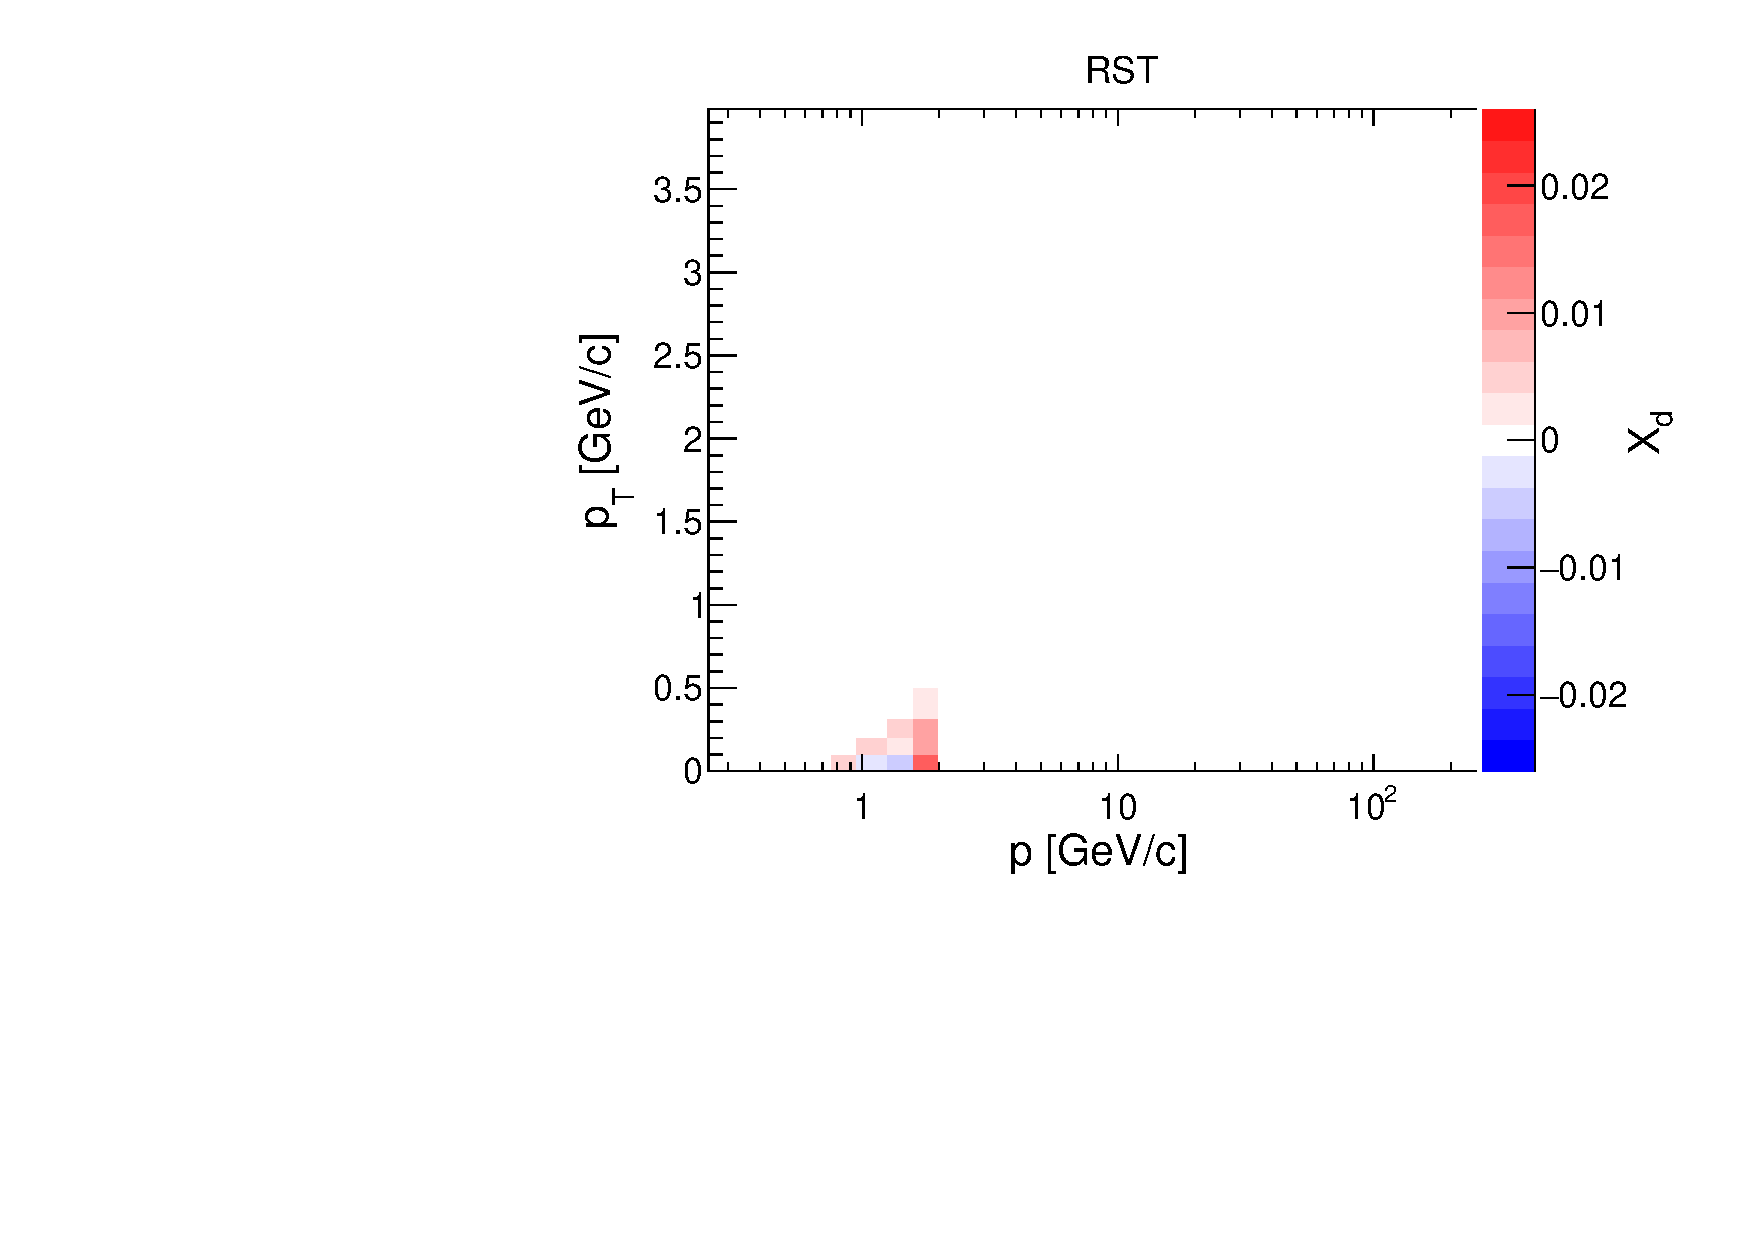
\includegraphics[clip, rviewport=0 0 1 0.94,width=0.4\textwidth]{dedx/model_350_v0_m5}
  \caption{Calibration constants obtained from the fit of the RST dataset at 350 \GeVc.}
  \label{fig:hadron:dedx:fit:cal350r}
\end{figure}

%%%%%%%%%% CAL %%%%%%%%%%%%%%
\begin{figure}
  \centering
  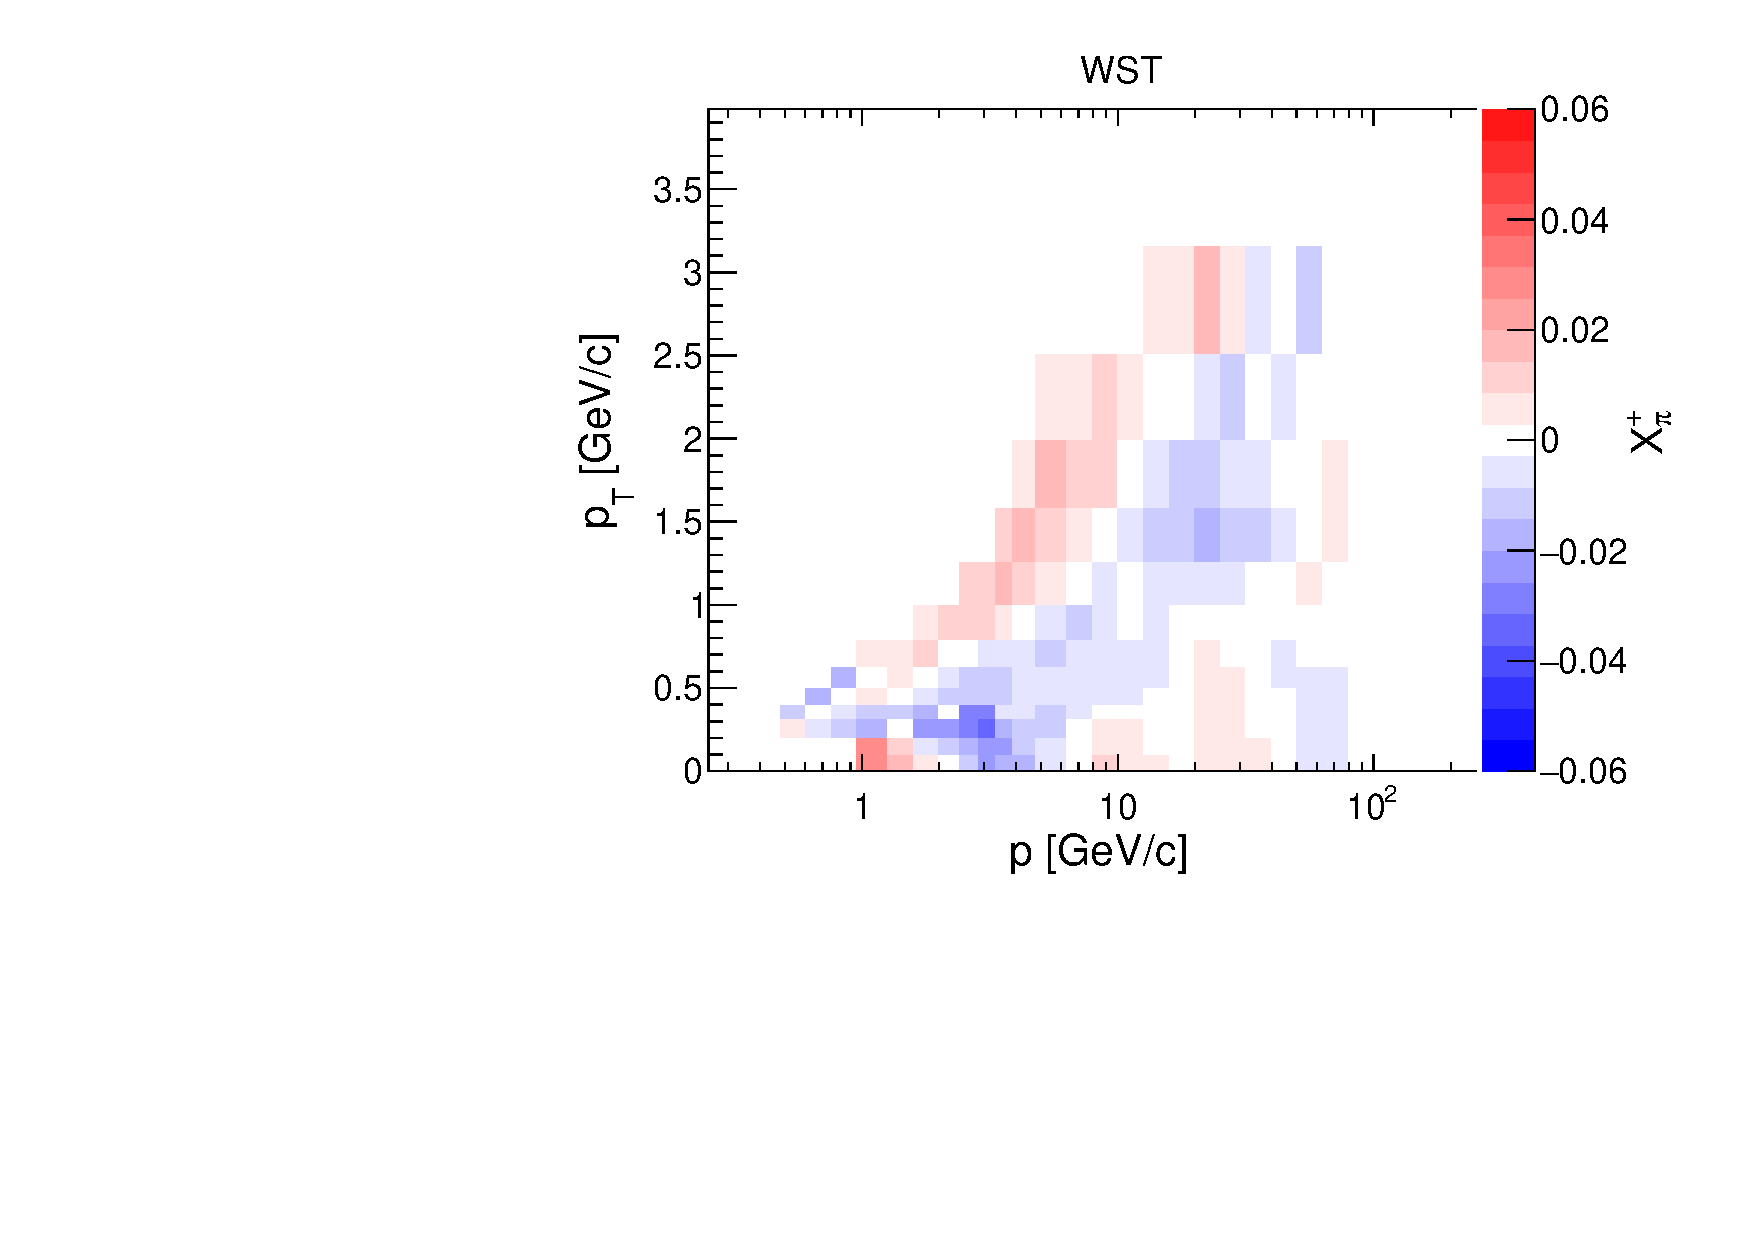
\includegraphics[clip, rviewport=0 0 1 0.94,width=0.4\textwidth]{dedx/model_350_v1_m0}
  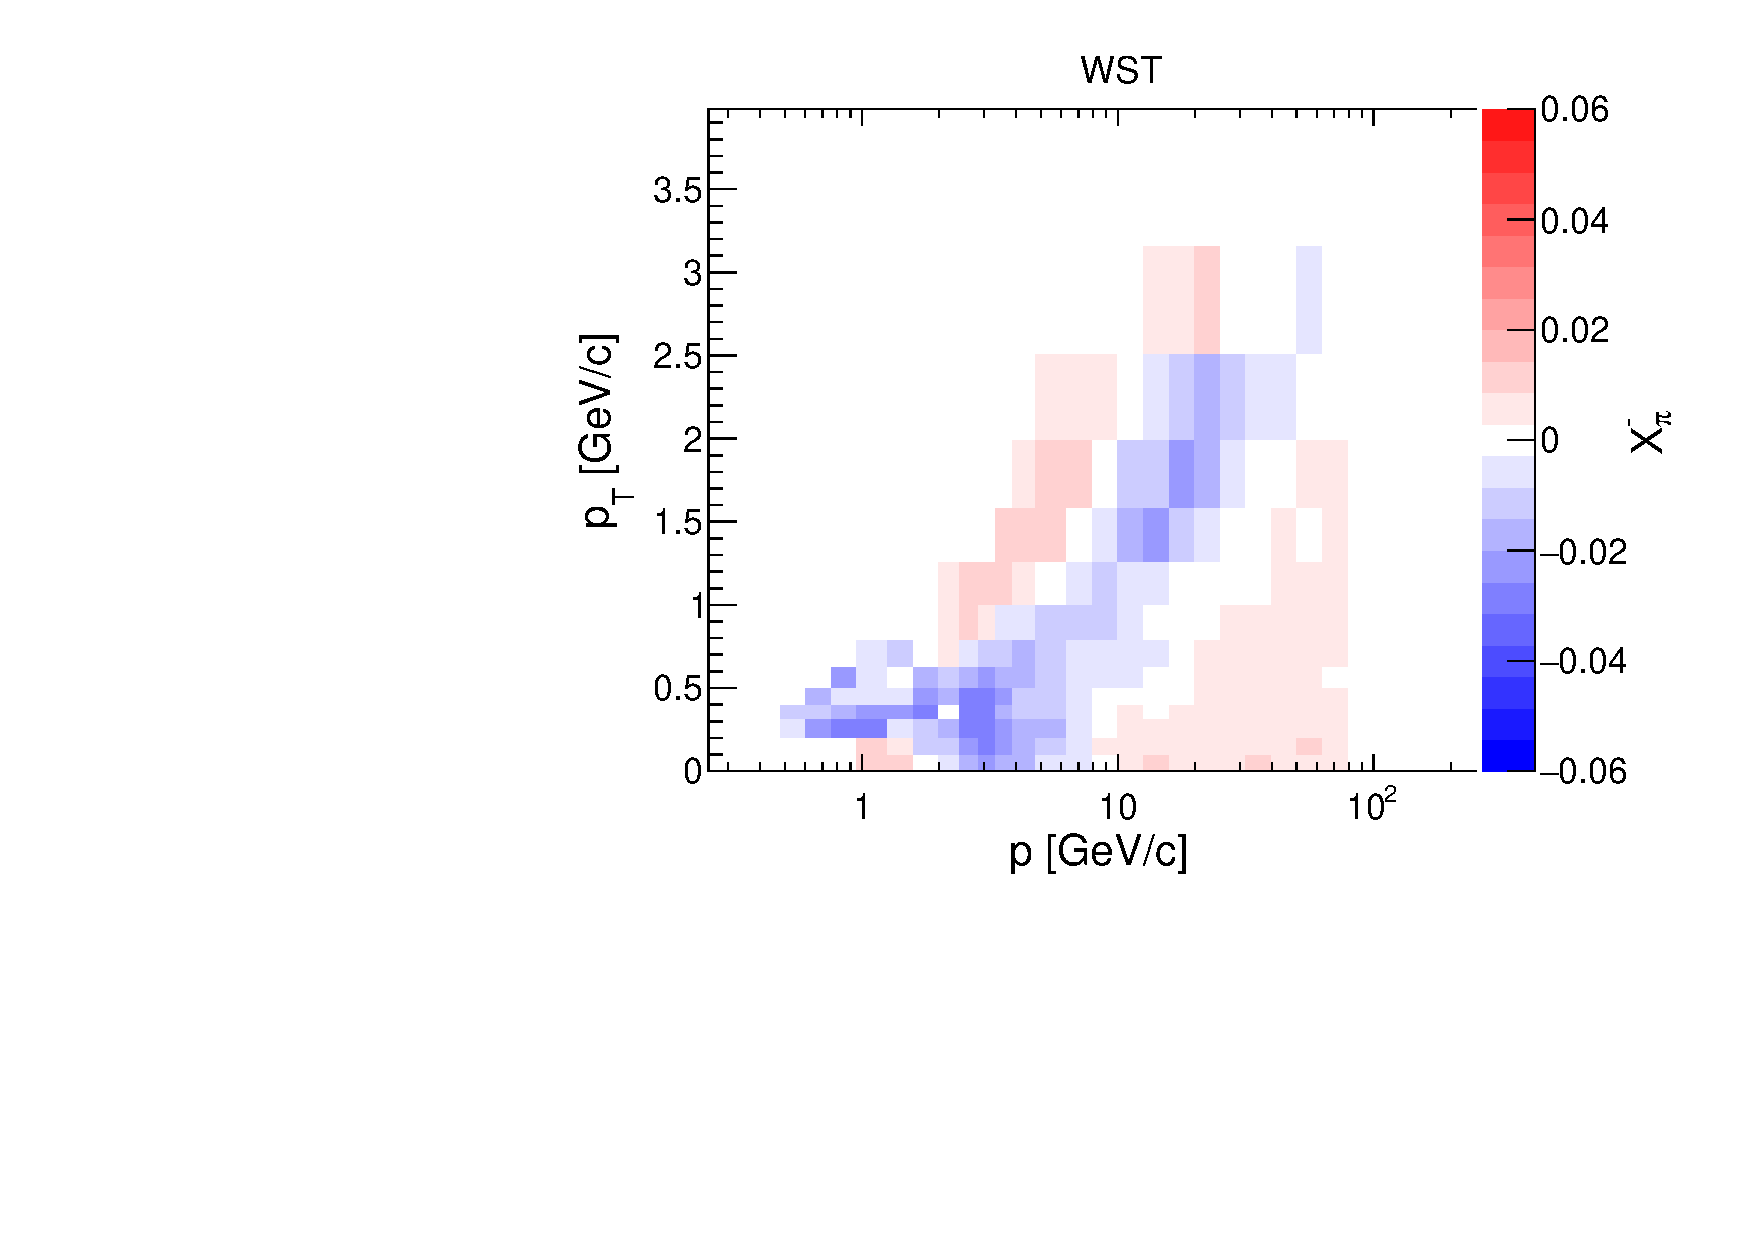
\includegraphics[clip, rviewport=0 0 1 0.94,width=0.4\textwidth]{dedx/model_350_v1_m1}

  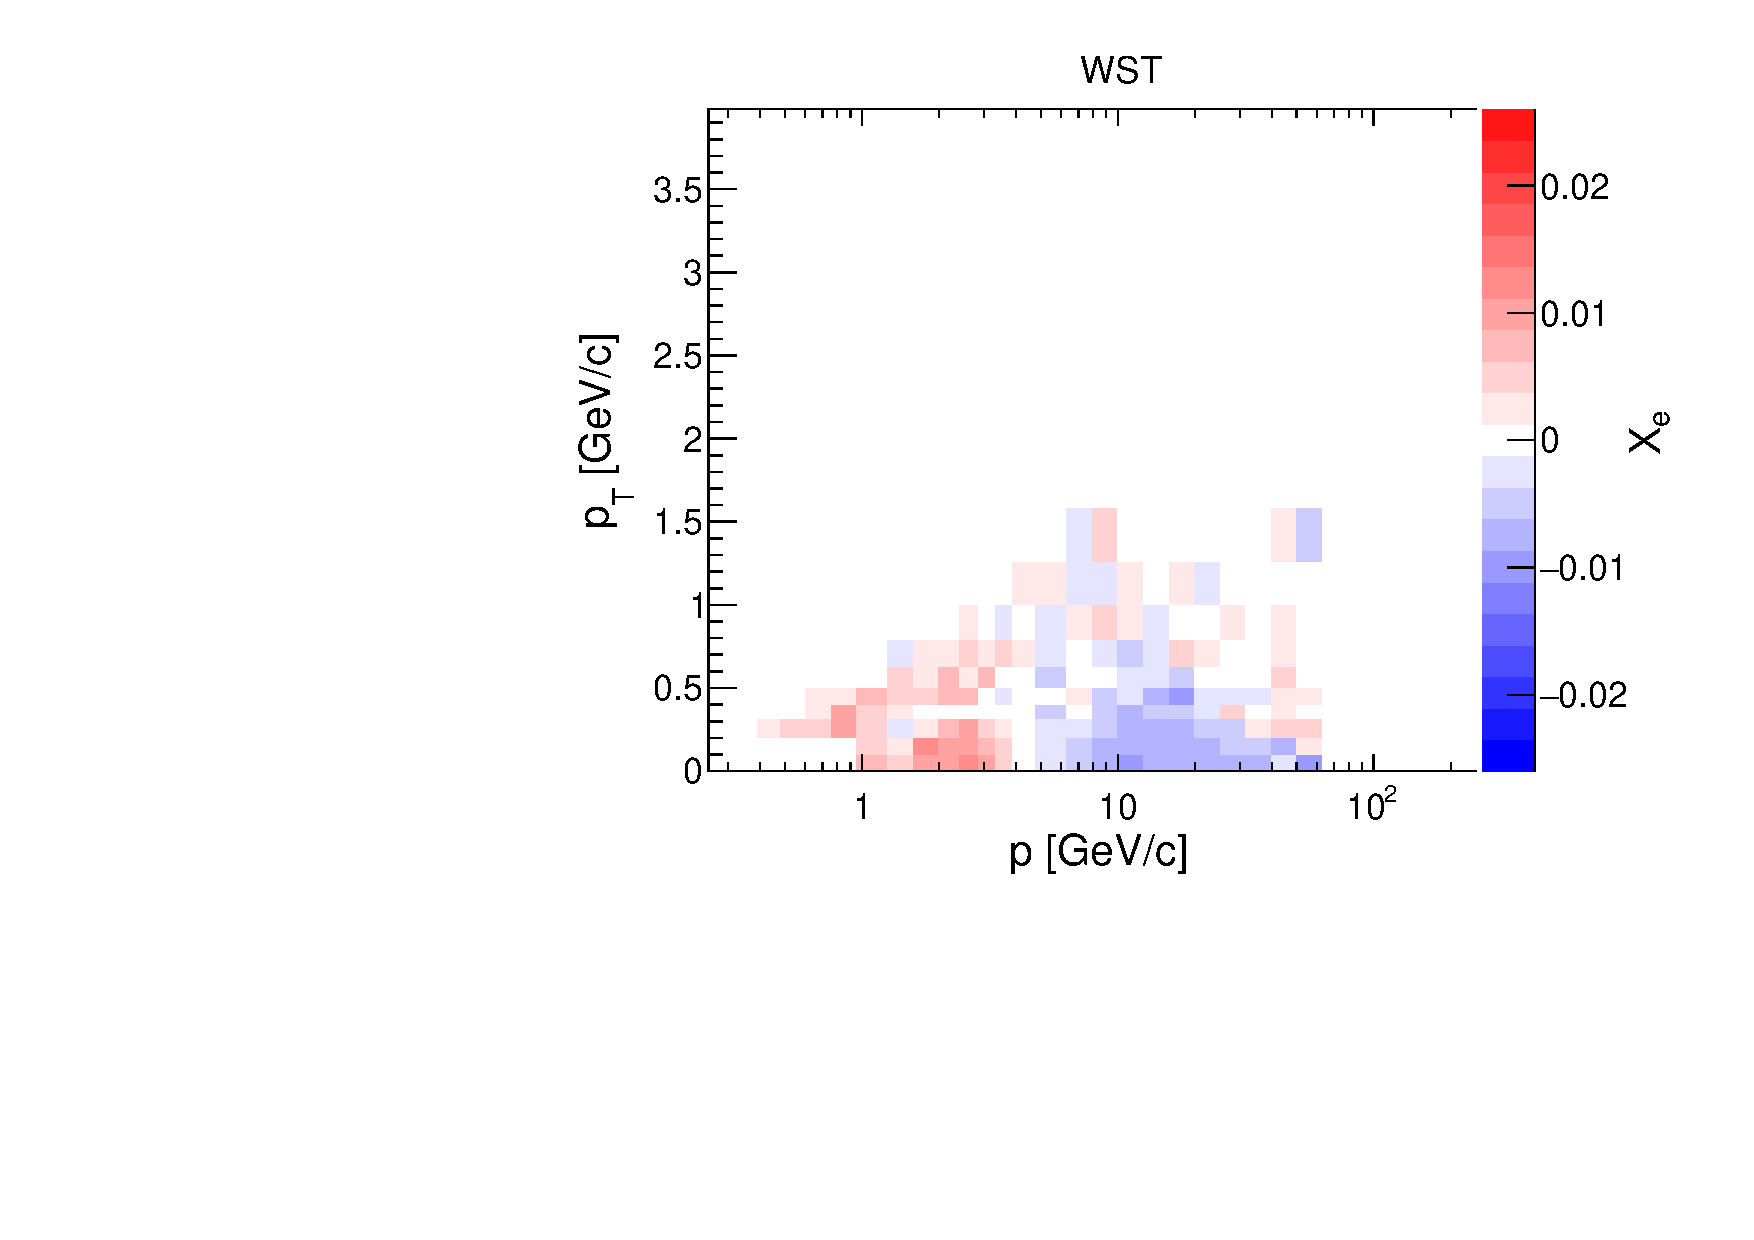
\includegraphics[clip, rviewport=0 0 1 0.94,width=0.4\textwidth]{dedx/model_350_v1_m2}
  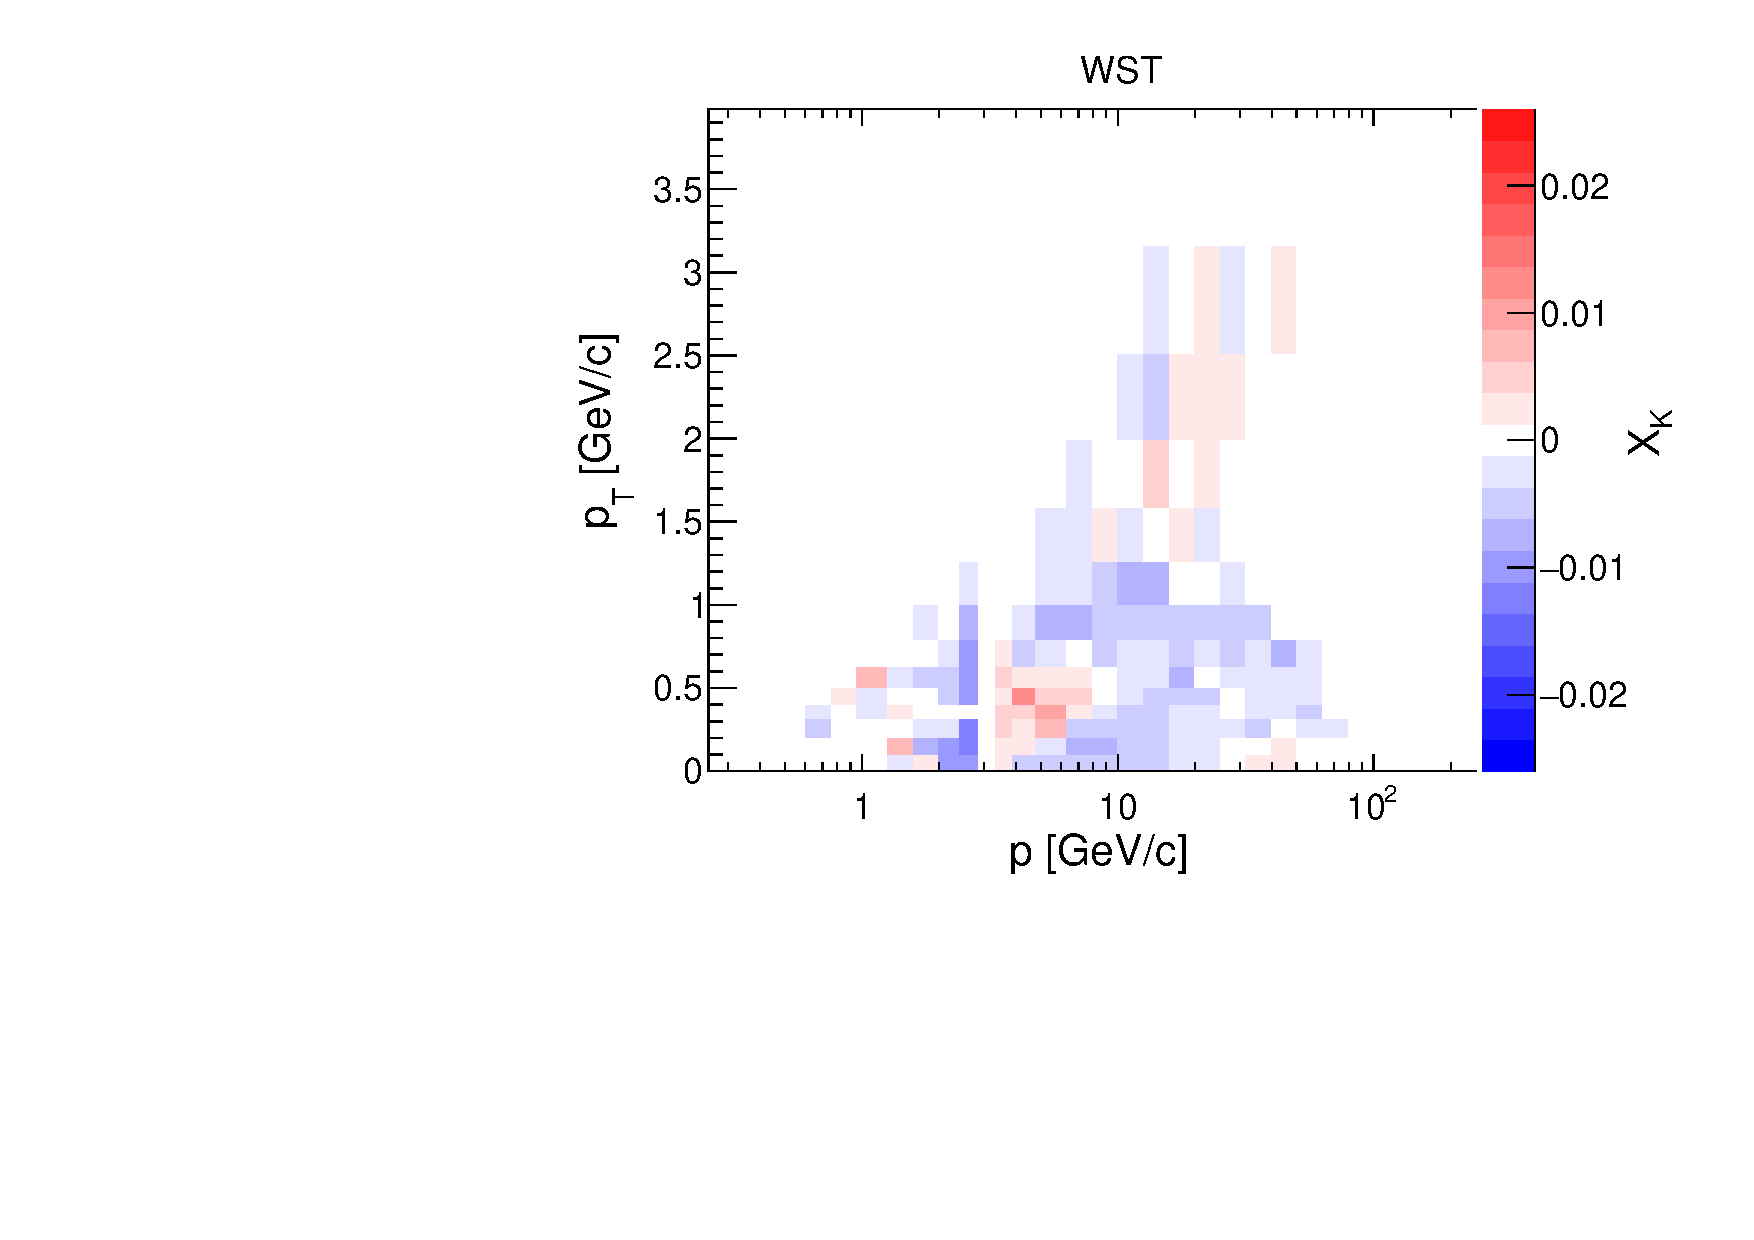
\includegraphics[clip, rviewport=0 0 1 0.94,width=0.4\textwidth]{dedx/model_350_v1_m3}

  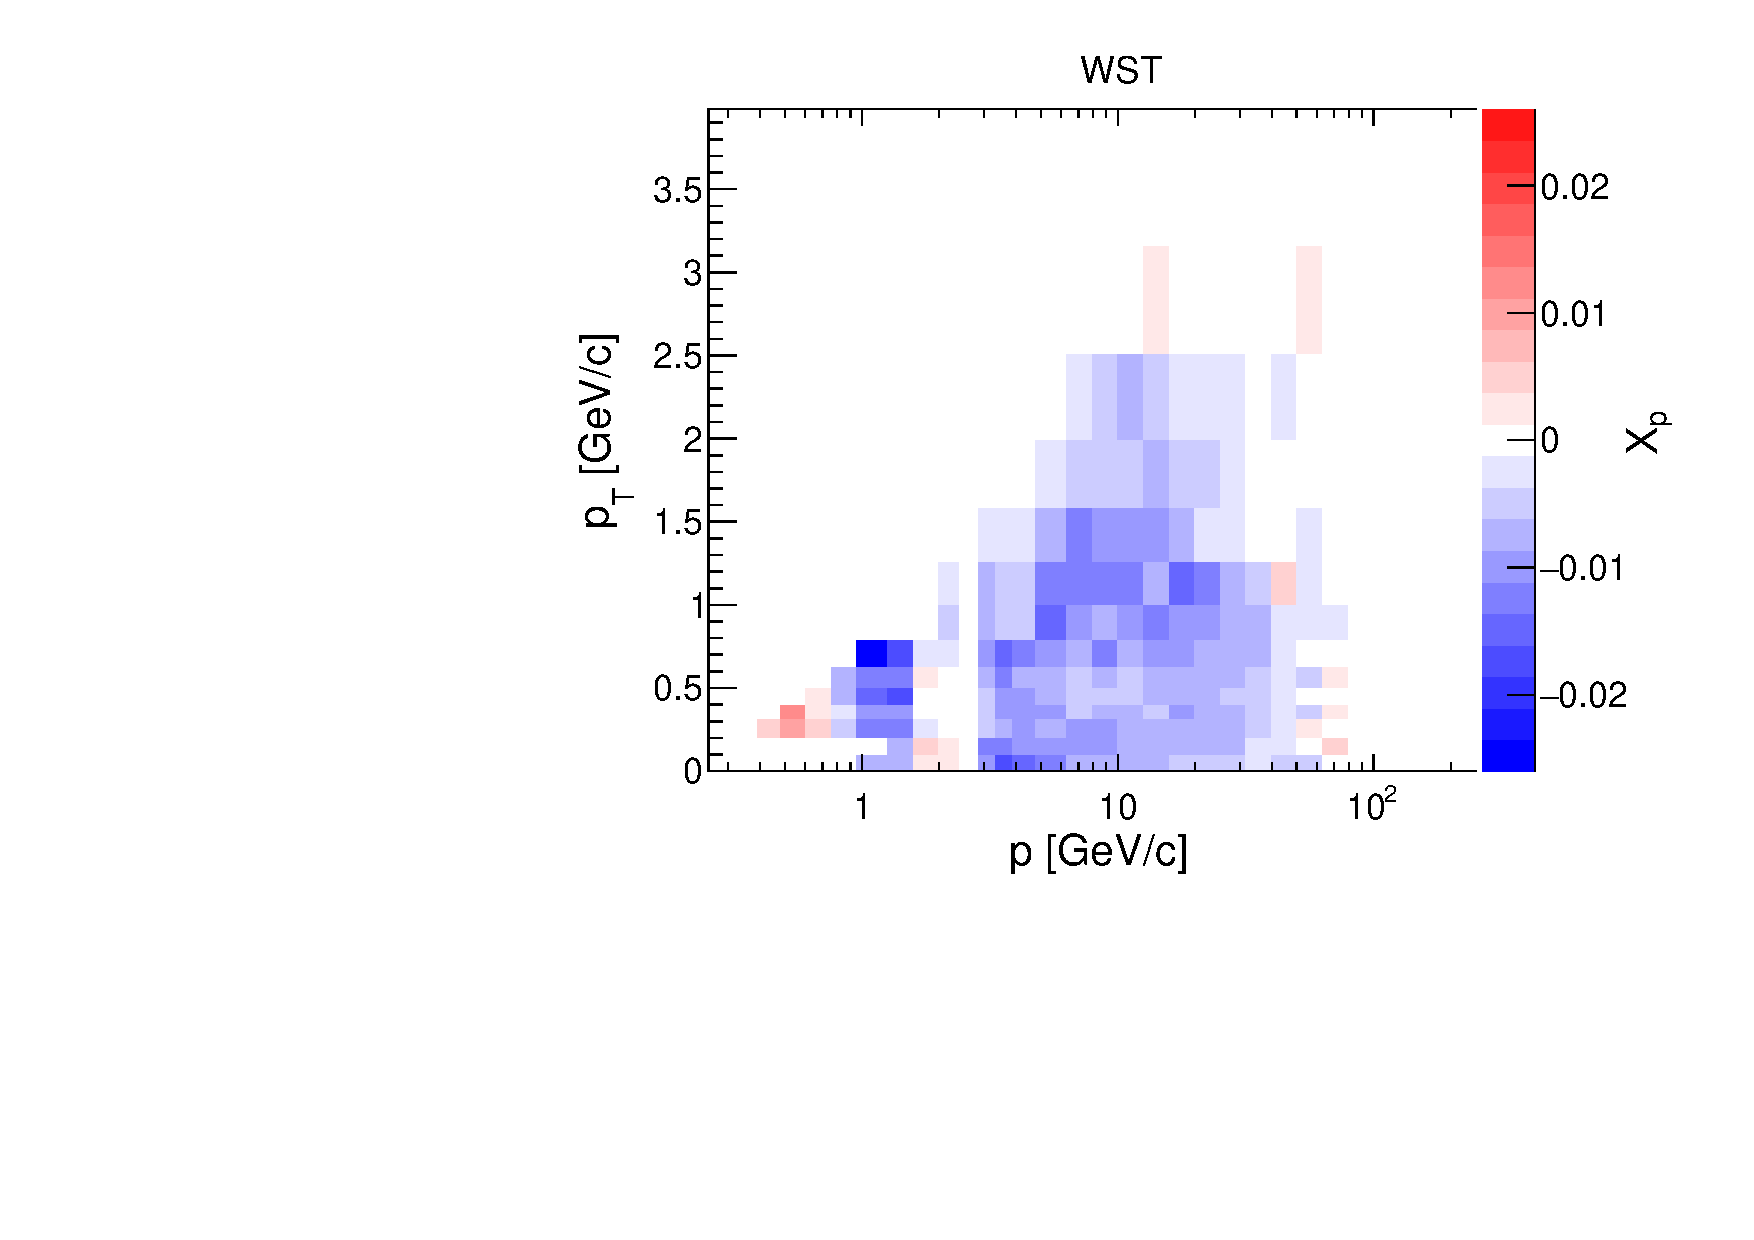
\includegraphics[clip, rviewport=0 0 1 0.94,width=0.4\textwidth]{dedx/model_350_v1_m4}
  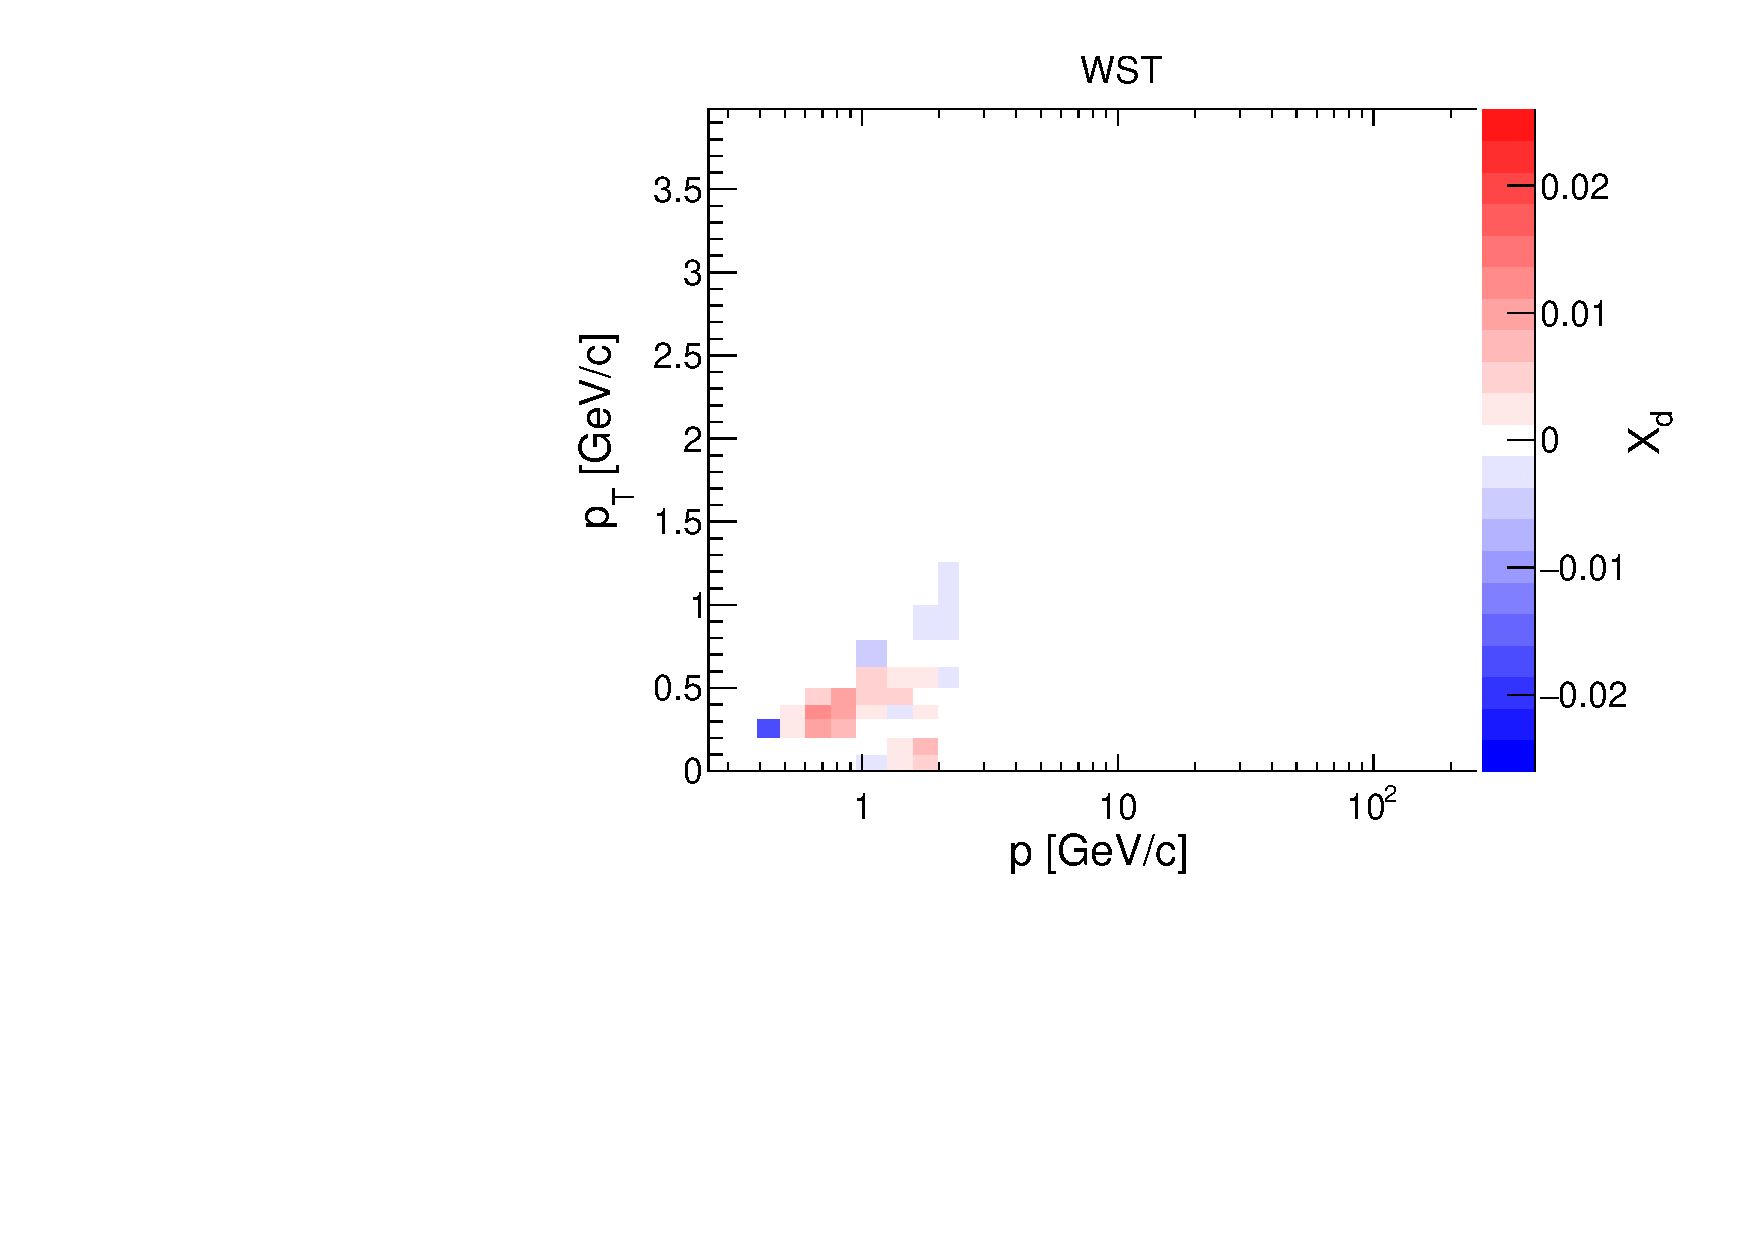
\includegraphics[clip, rviewport=0 0 1 0.94,width=0.4\textwidth]{dedx/model_350_v1_m5}
  \caption{Calibration constants obtained from the fit of the WST dataset at 350 \GeVc.}
  \label{fig:hadron:dedx:fit:cal350w}
\end{figure}

\clearpage

%%%%%%%%%% SHAPE %%%%%%%%%%%%%%
\begin{figure}
  \centering
  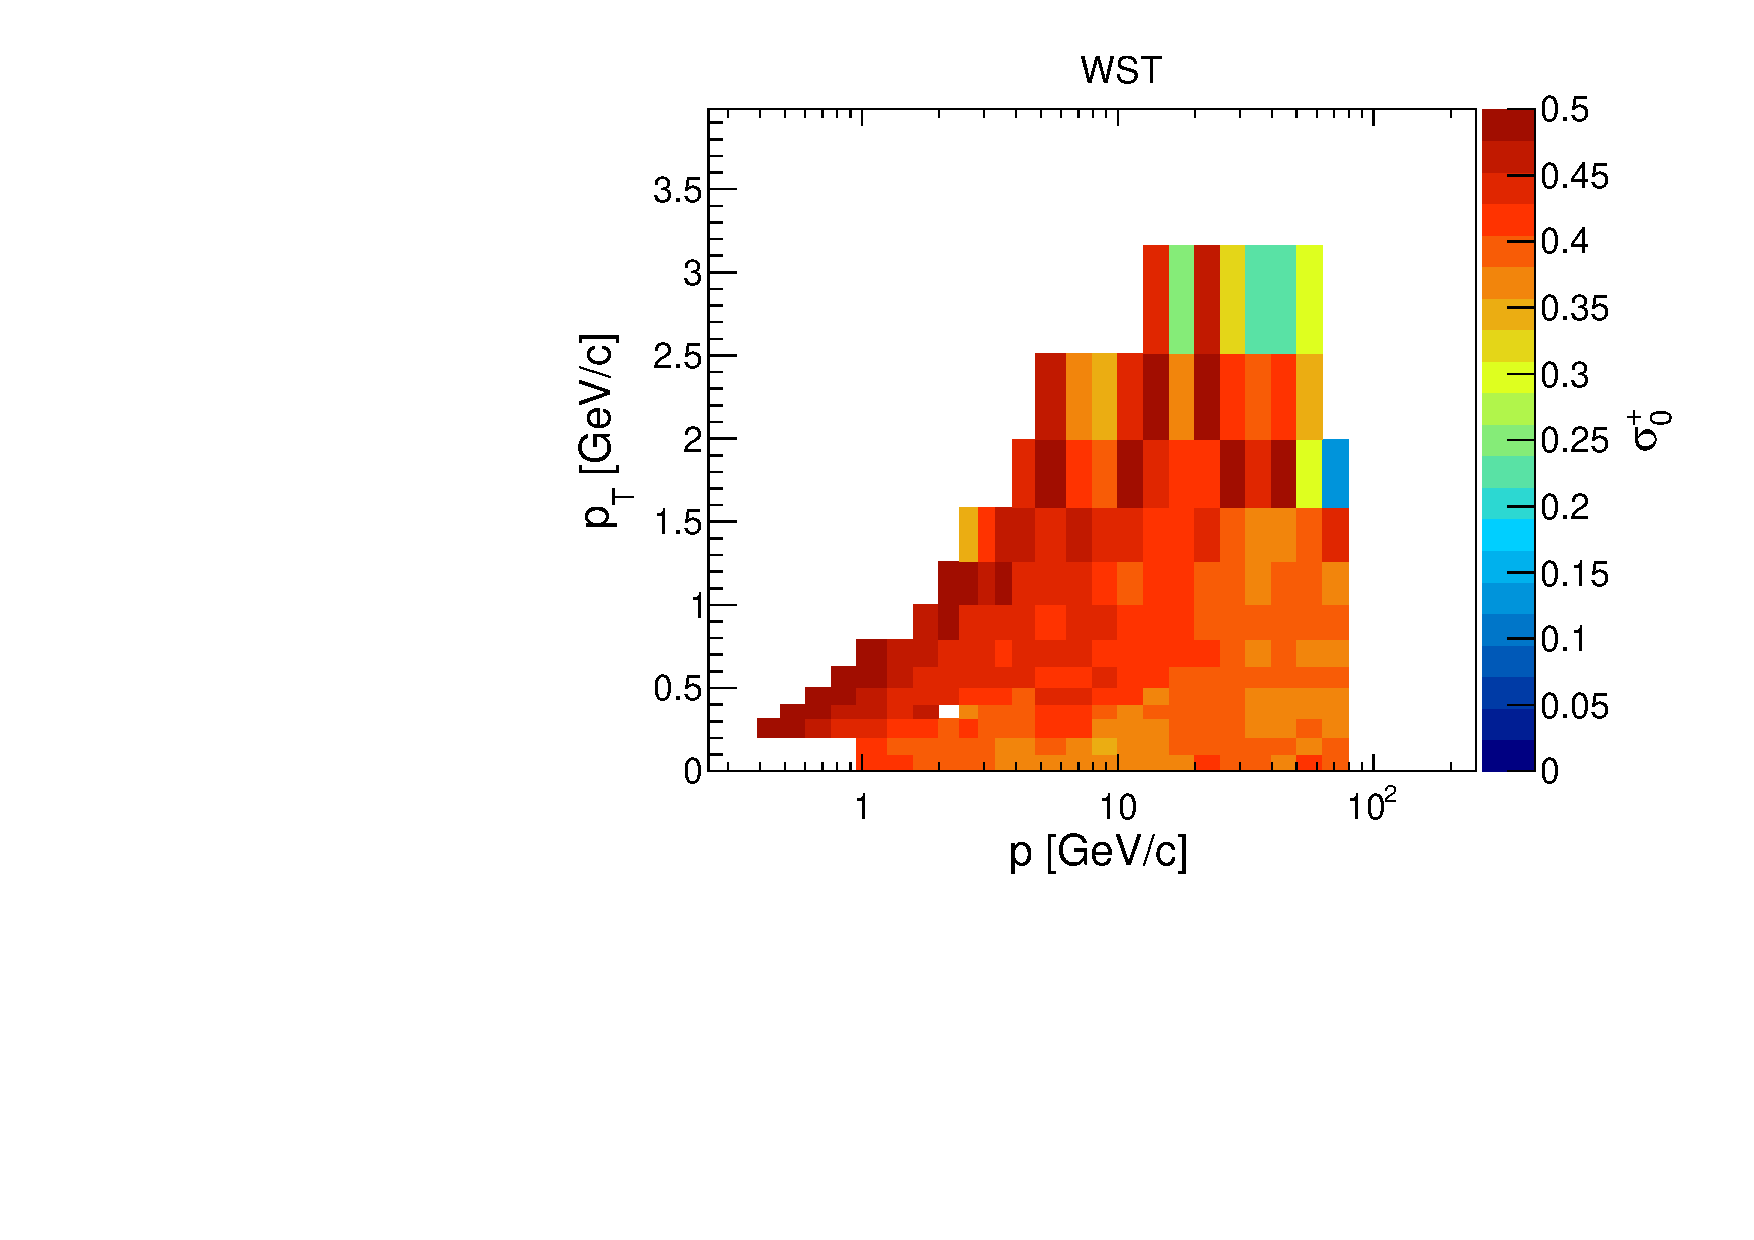
\includegraphics[clip, rviewport=0 0 1 0.94,width=0.4\textwidth]{dedx/model_158_v1_m6}
  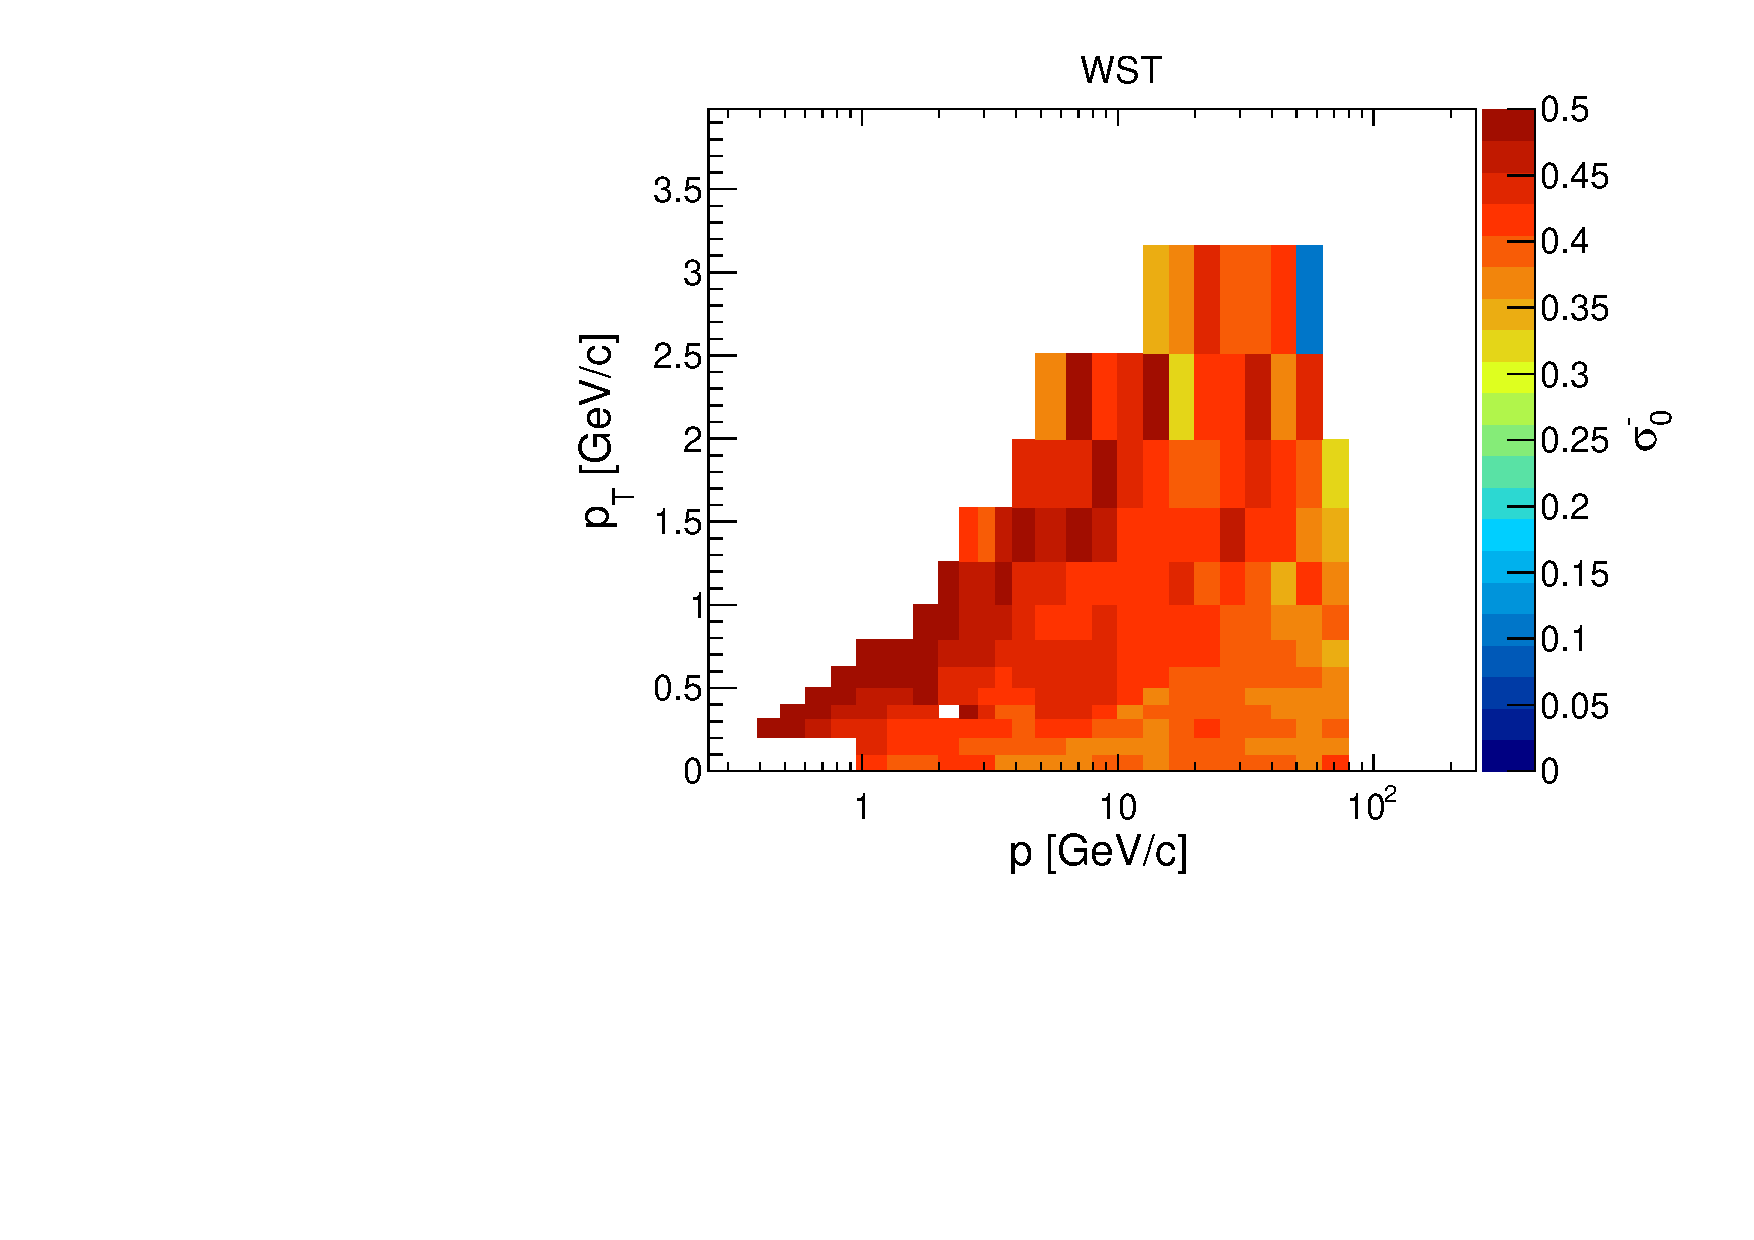
\includegraphics[clip, rviewport=0 0 1 0.94,width=0.4\textwidth]{dedx/model_158_v1_m7}

  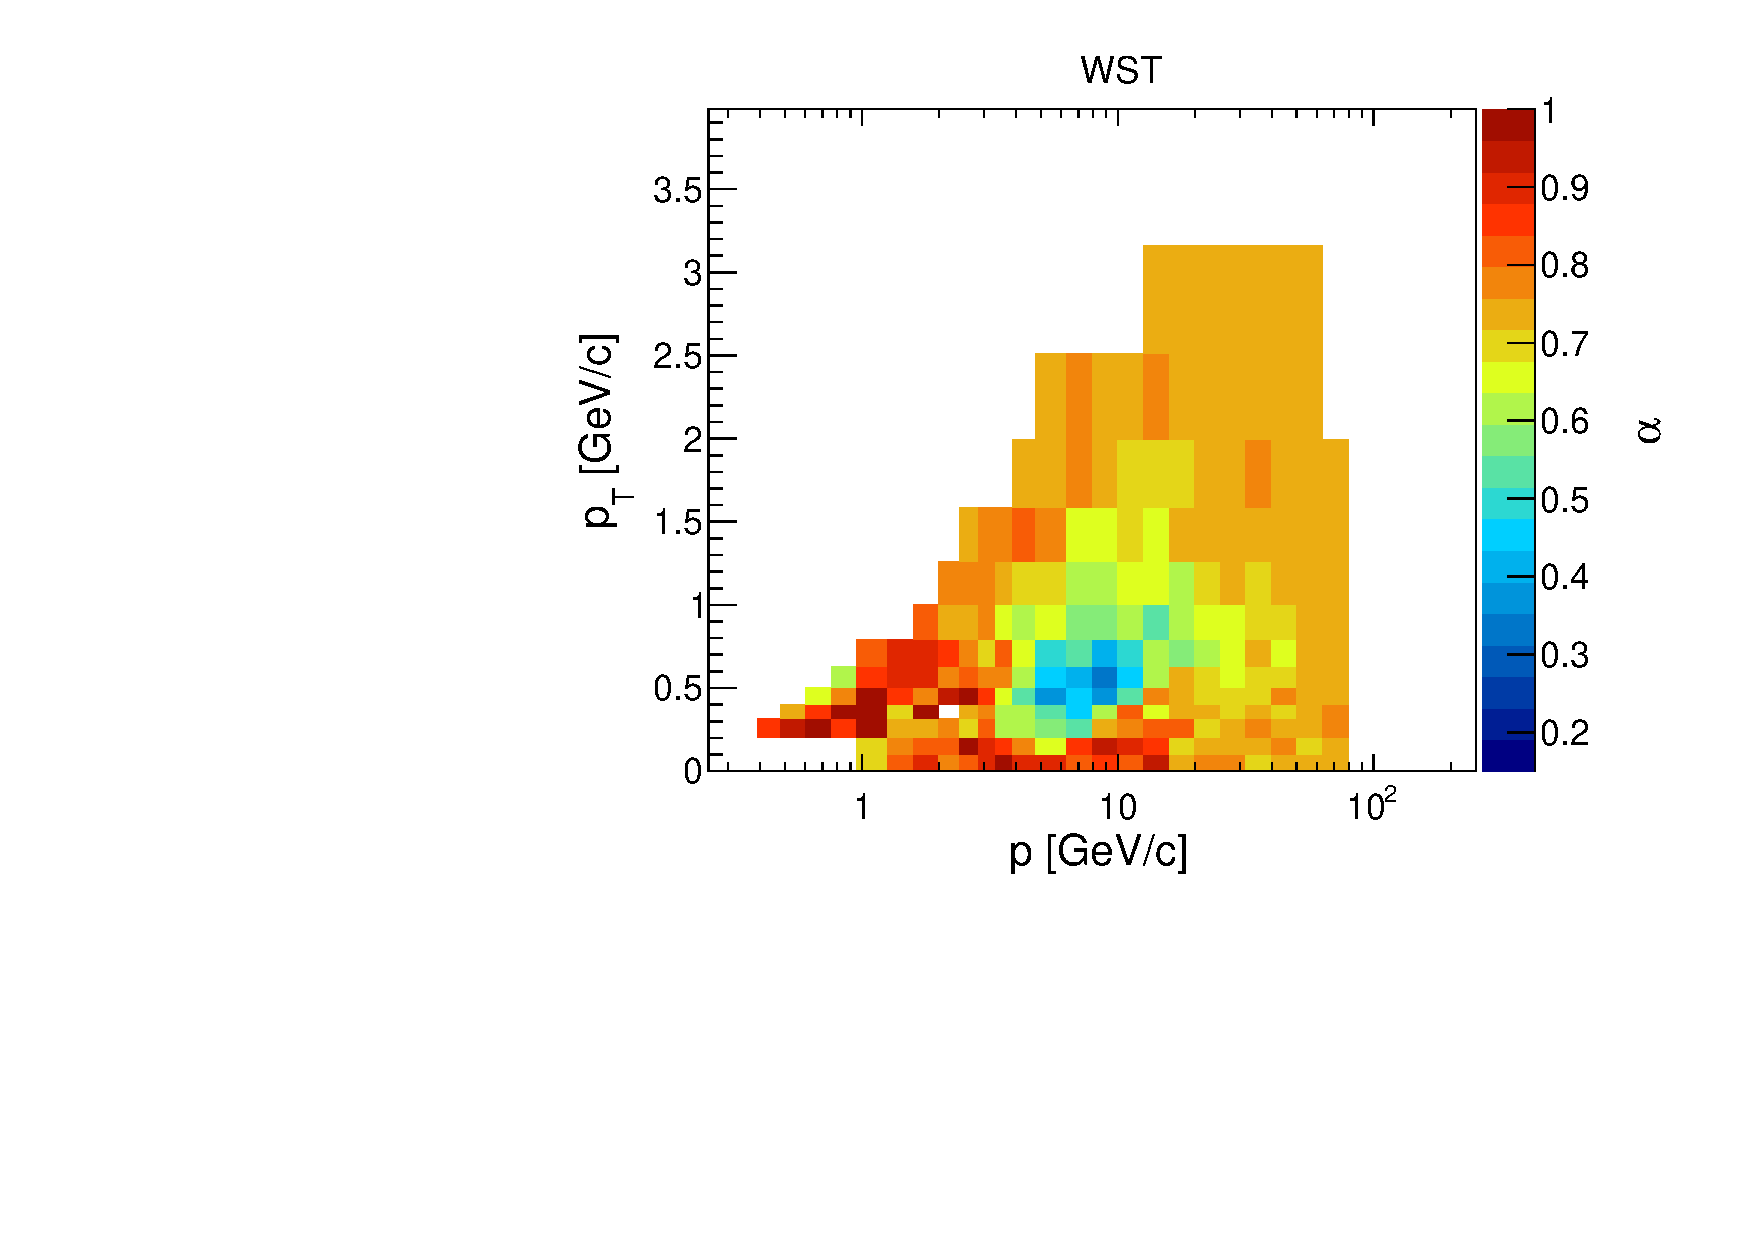
\includegraphics[clip, rviewport=0 0 1 0.94,width=0.4\textwidth]{dedx/model_158_v1_m9}
  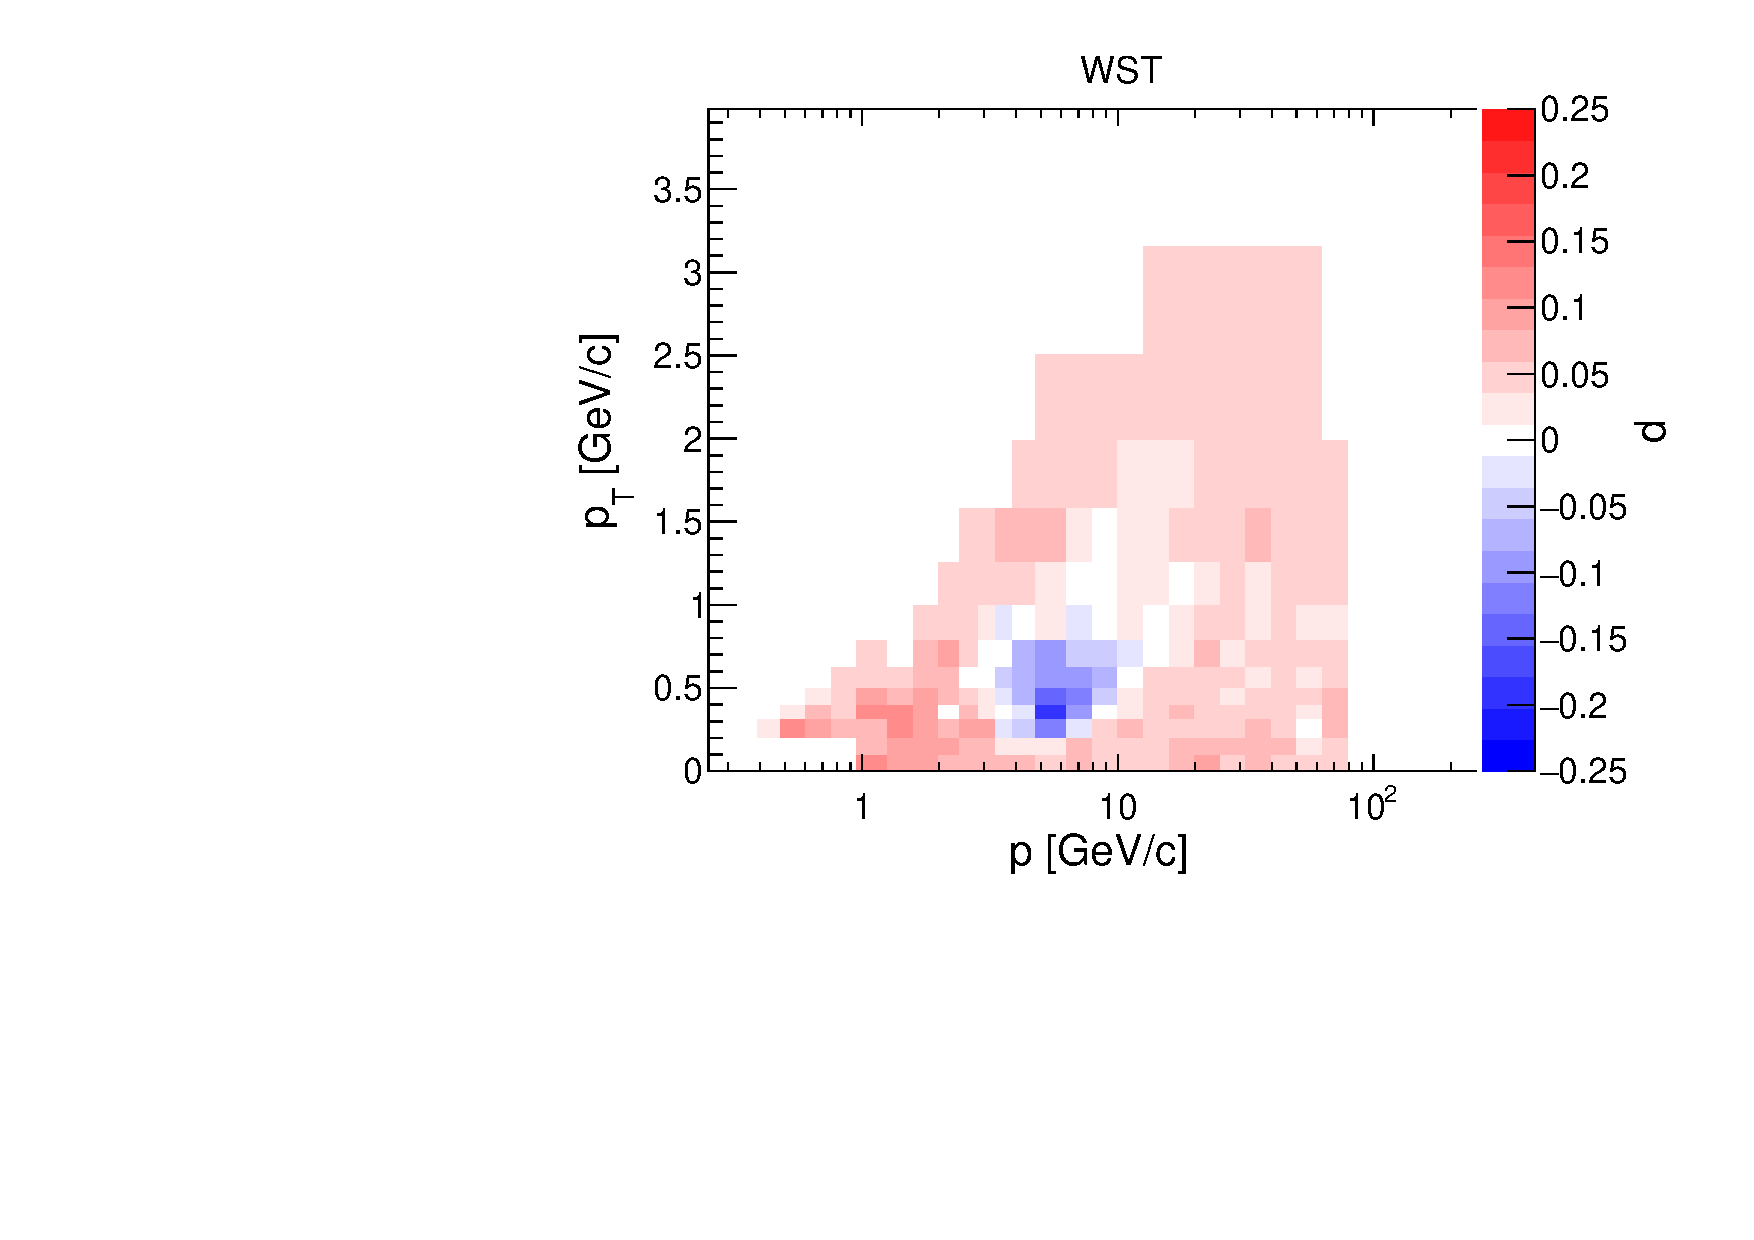
\includegraphics[clip, rviewport=0 0 1 0.94,width=0.4\textwidth]{dedx/model_158_v1_m10}
  \caption{Shape parameters obtained from the fit of the WST dataset at 158 \GeVc.}
  \label{fig:hadron:dedx:fit:shape158w}
\end{figure}

%%%%%%%%%% SHAPE %%%%%%%%%%%%%%
\begin{figure}
  \centering
  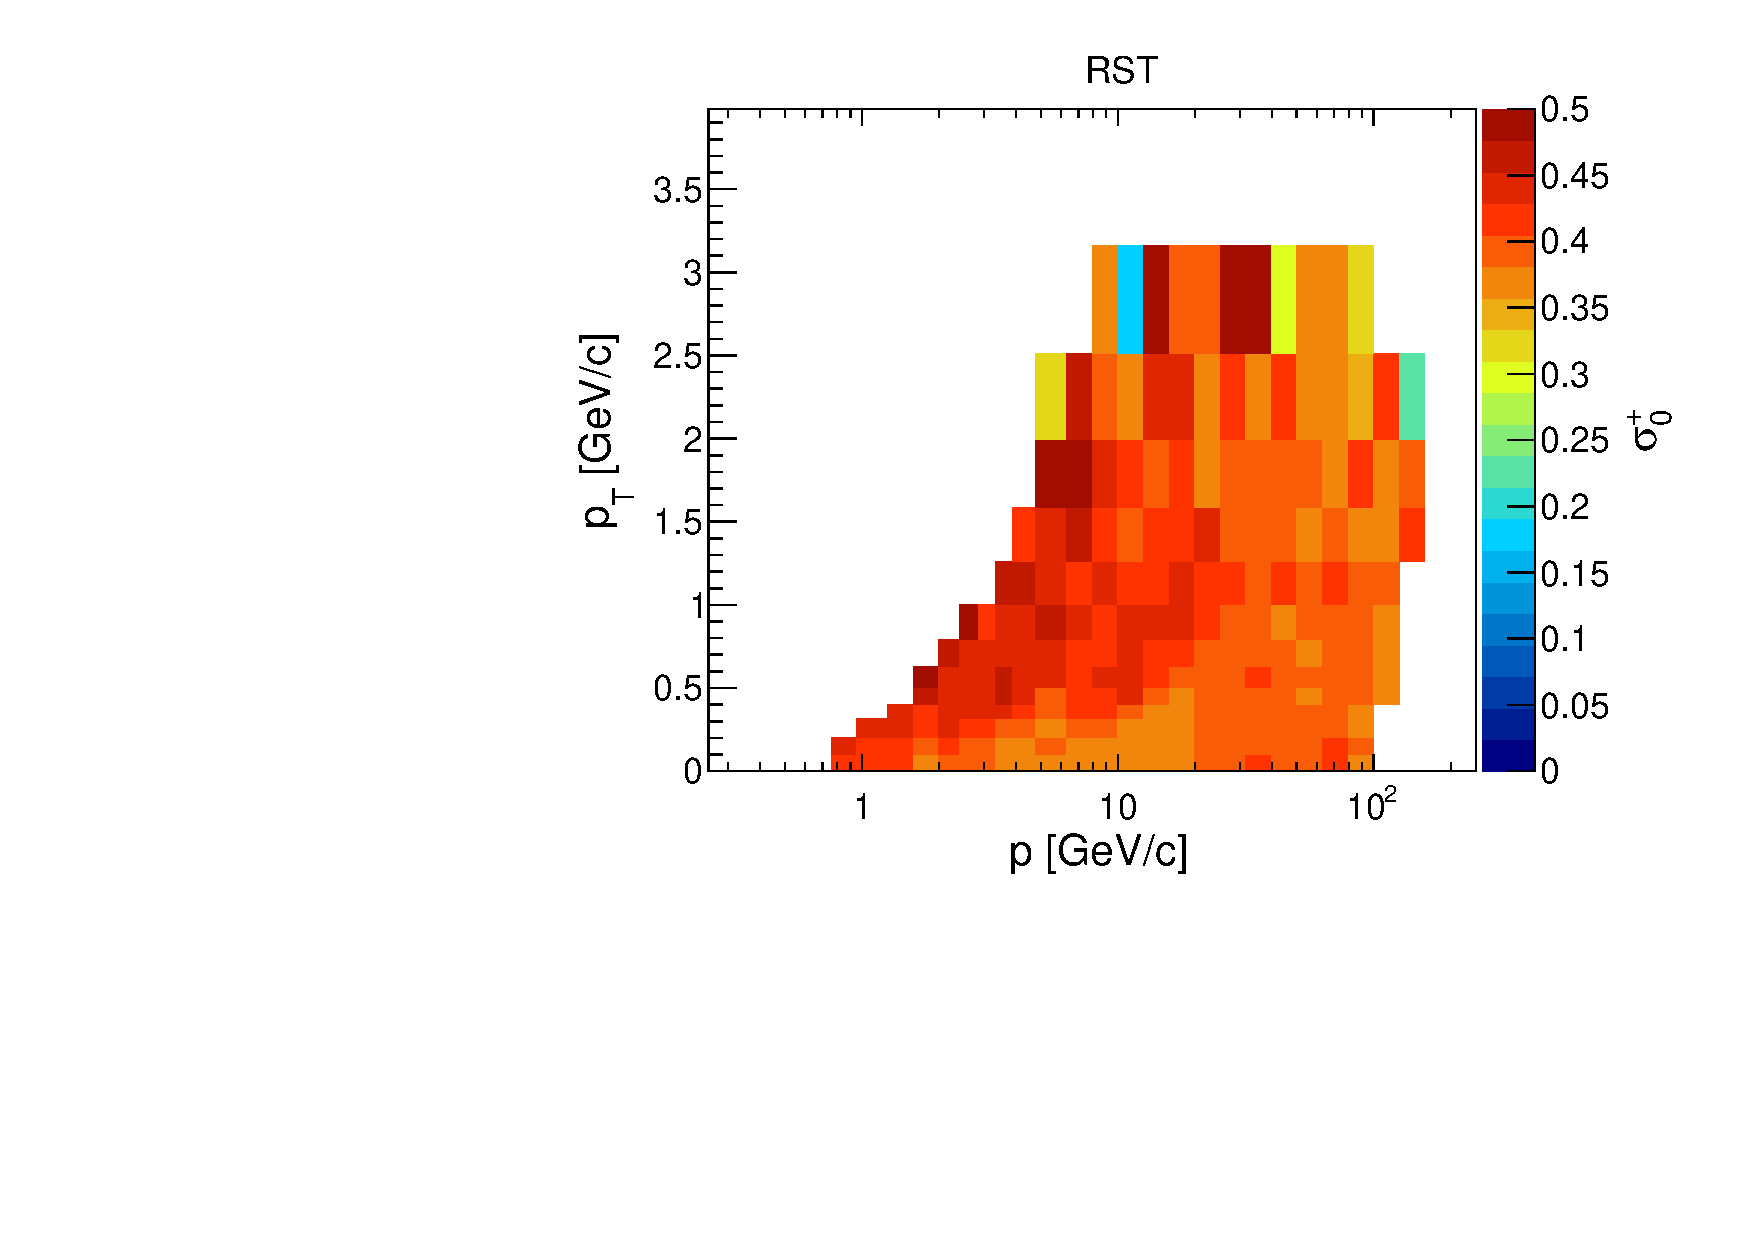
\includegraphics[clip, rviewport=0 0 1 0.94,width=0.4\textwidth]{dedx/model_350_v0_m6}
  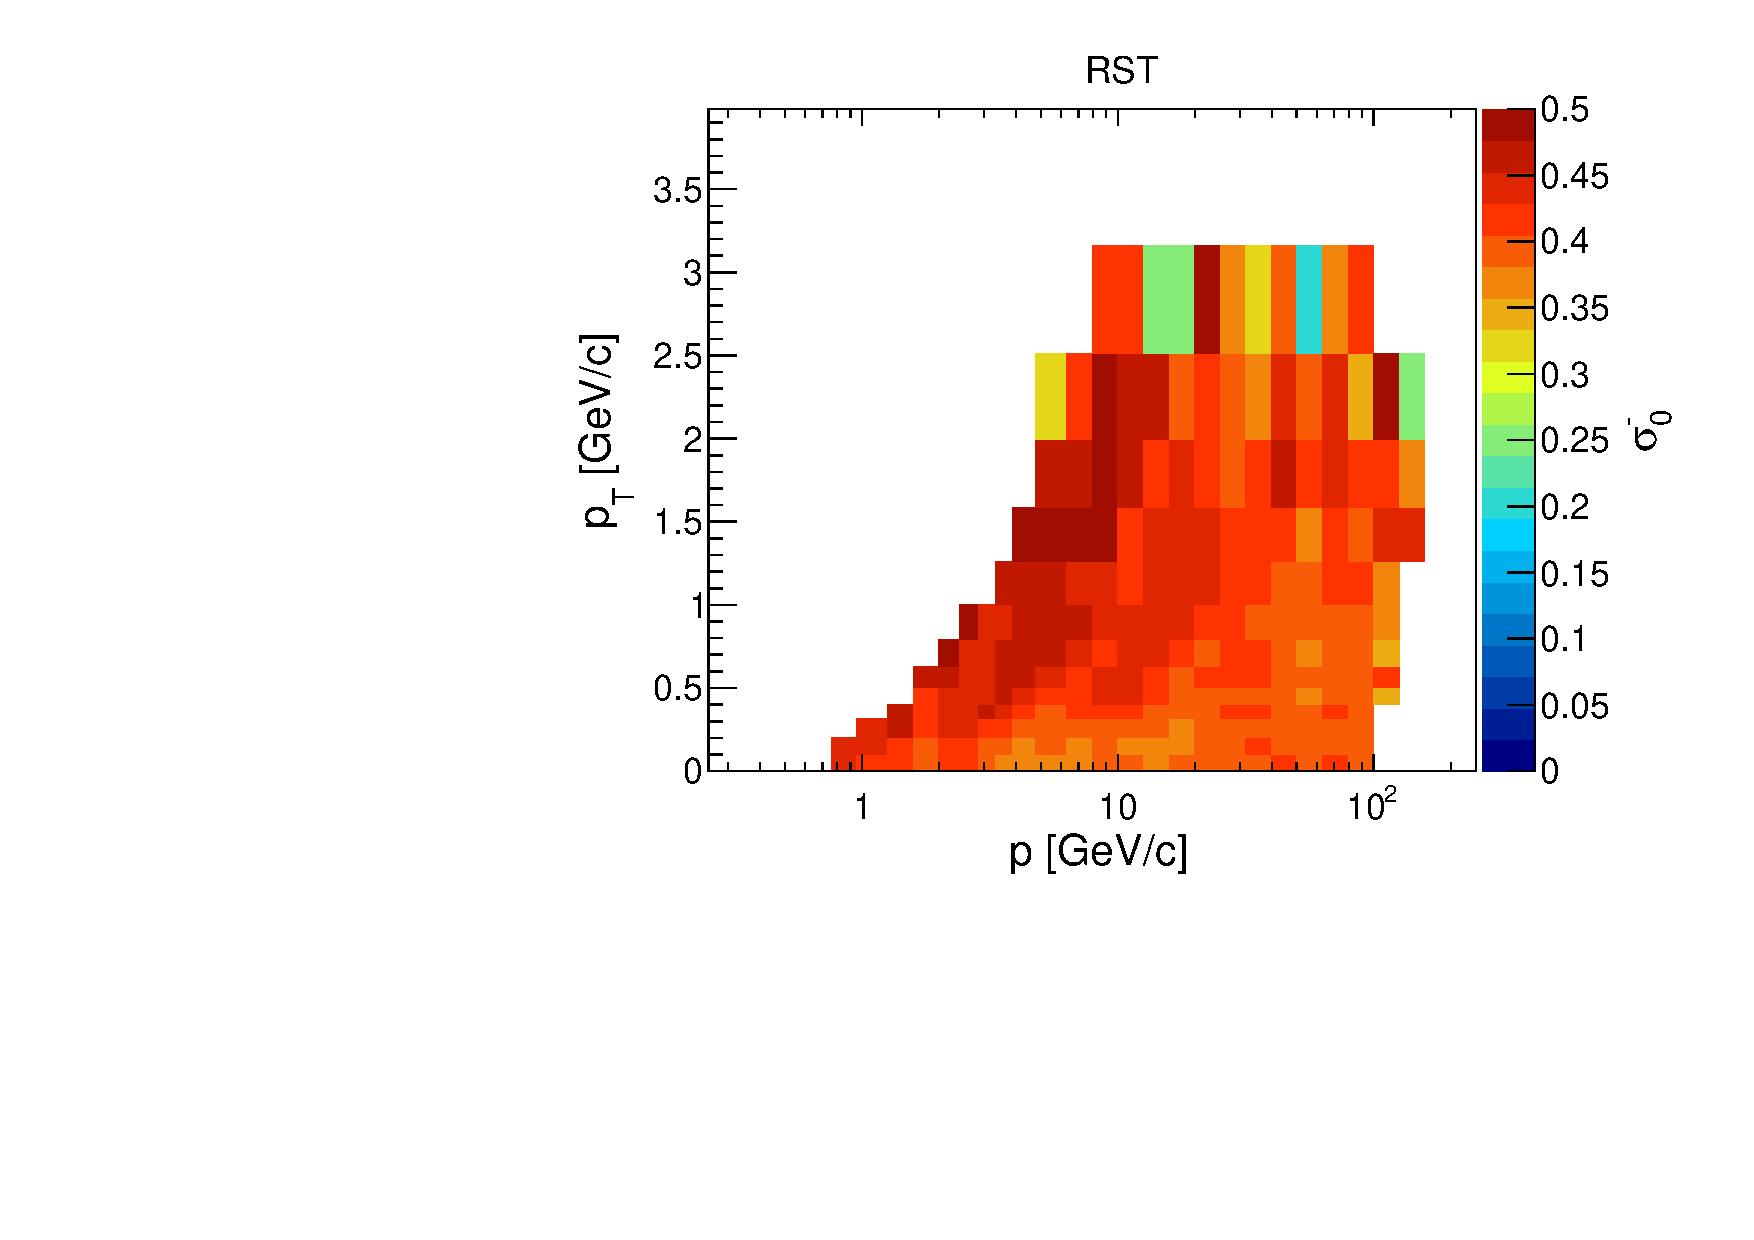
\includegraphics[clip, rviewport=0 0 1 0.94,width=0.4\textwidth]{dedx/model_350_v0_m7}

  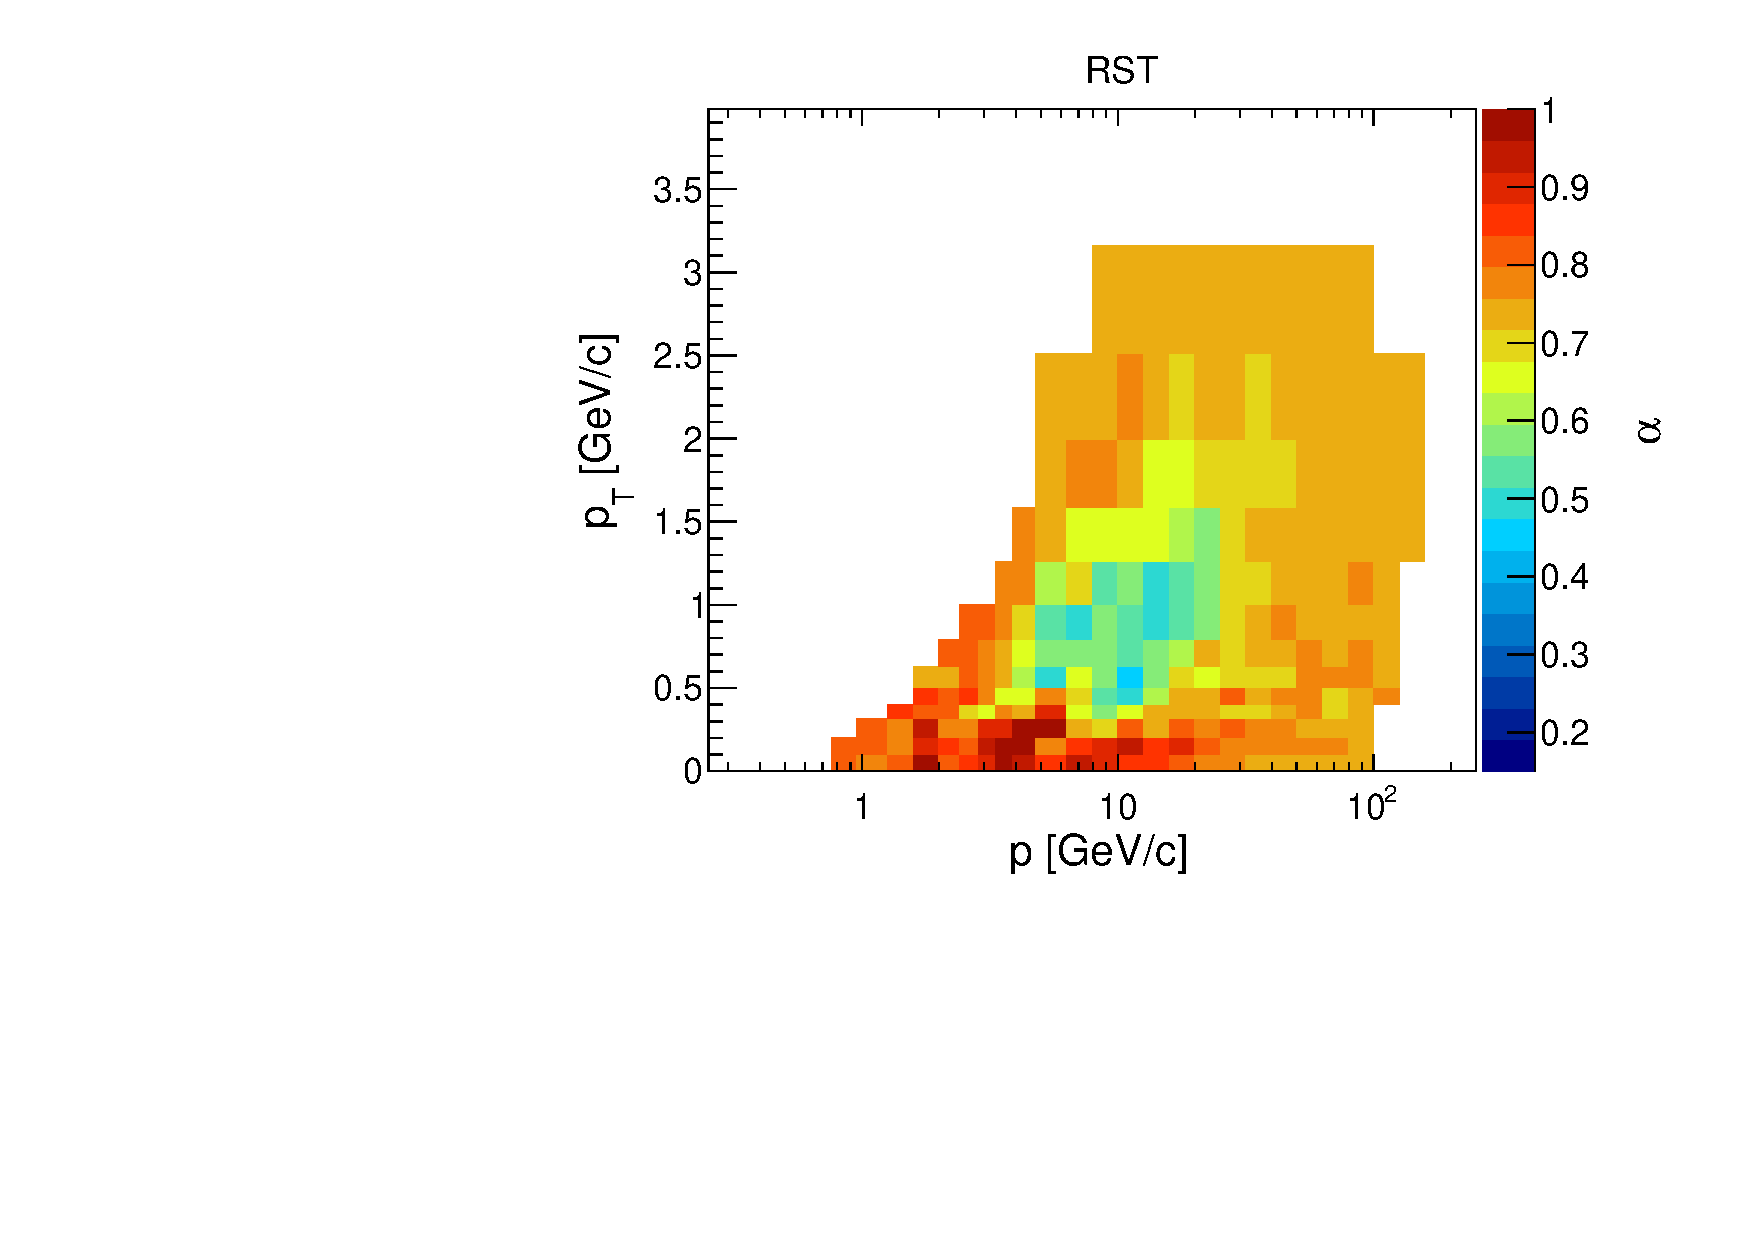
\includegraphics[clip, rviewport=0 0 1 0.94,width=0.4\textwidth]{dedx/model_350_v0_m9}
  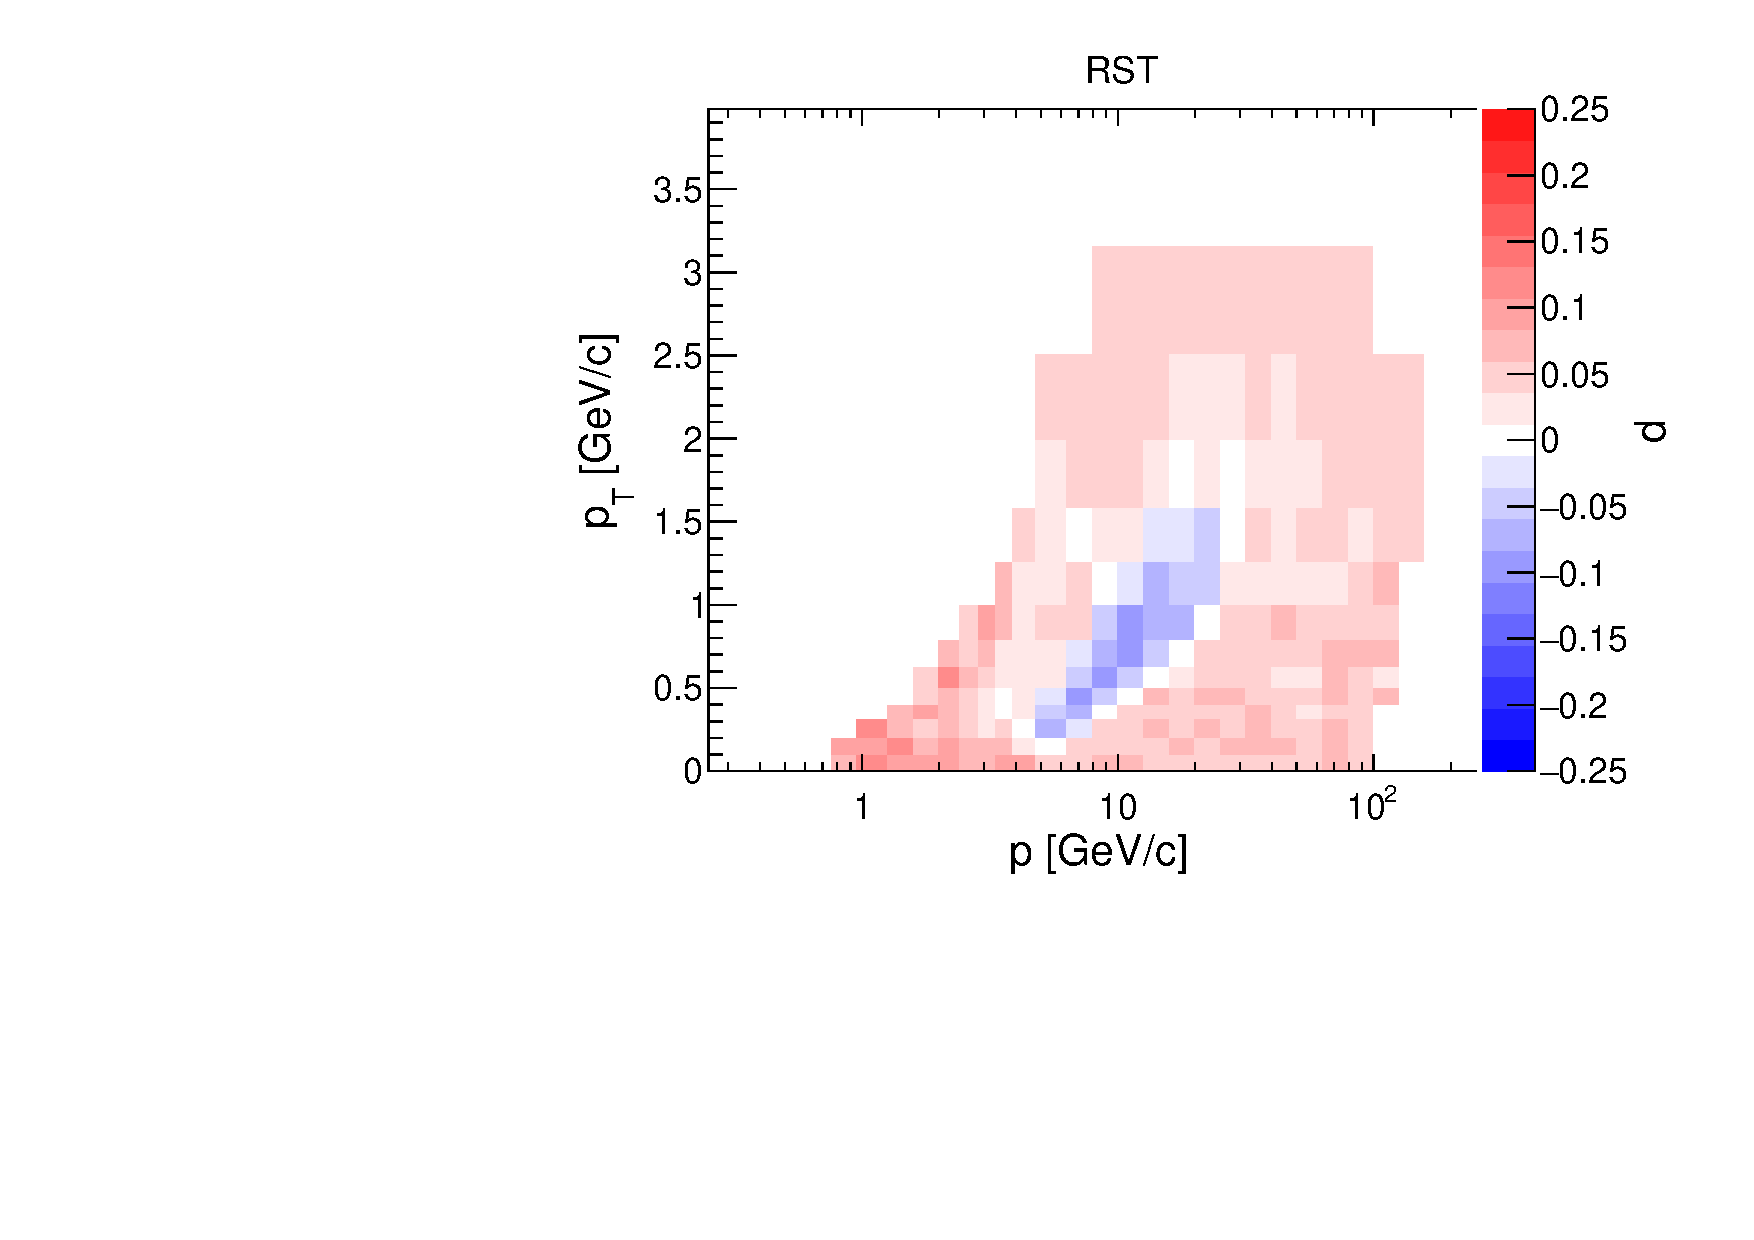
\includegraphics[clip, rviewport=0 0 1 0.94,width=0.4\textwidth]{dedx/model_350_v0_m10}
  \caption{Shape parameters obtained from the fit of the RST dataset at 350 \GeVc.}
  \label{fig:hadron:dedx:fit:shape350r}
\end{figure}

%%%%%%%%%% SHAPE %%%%%%%%%%%%%%
\begin{figure}
  \centering
  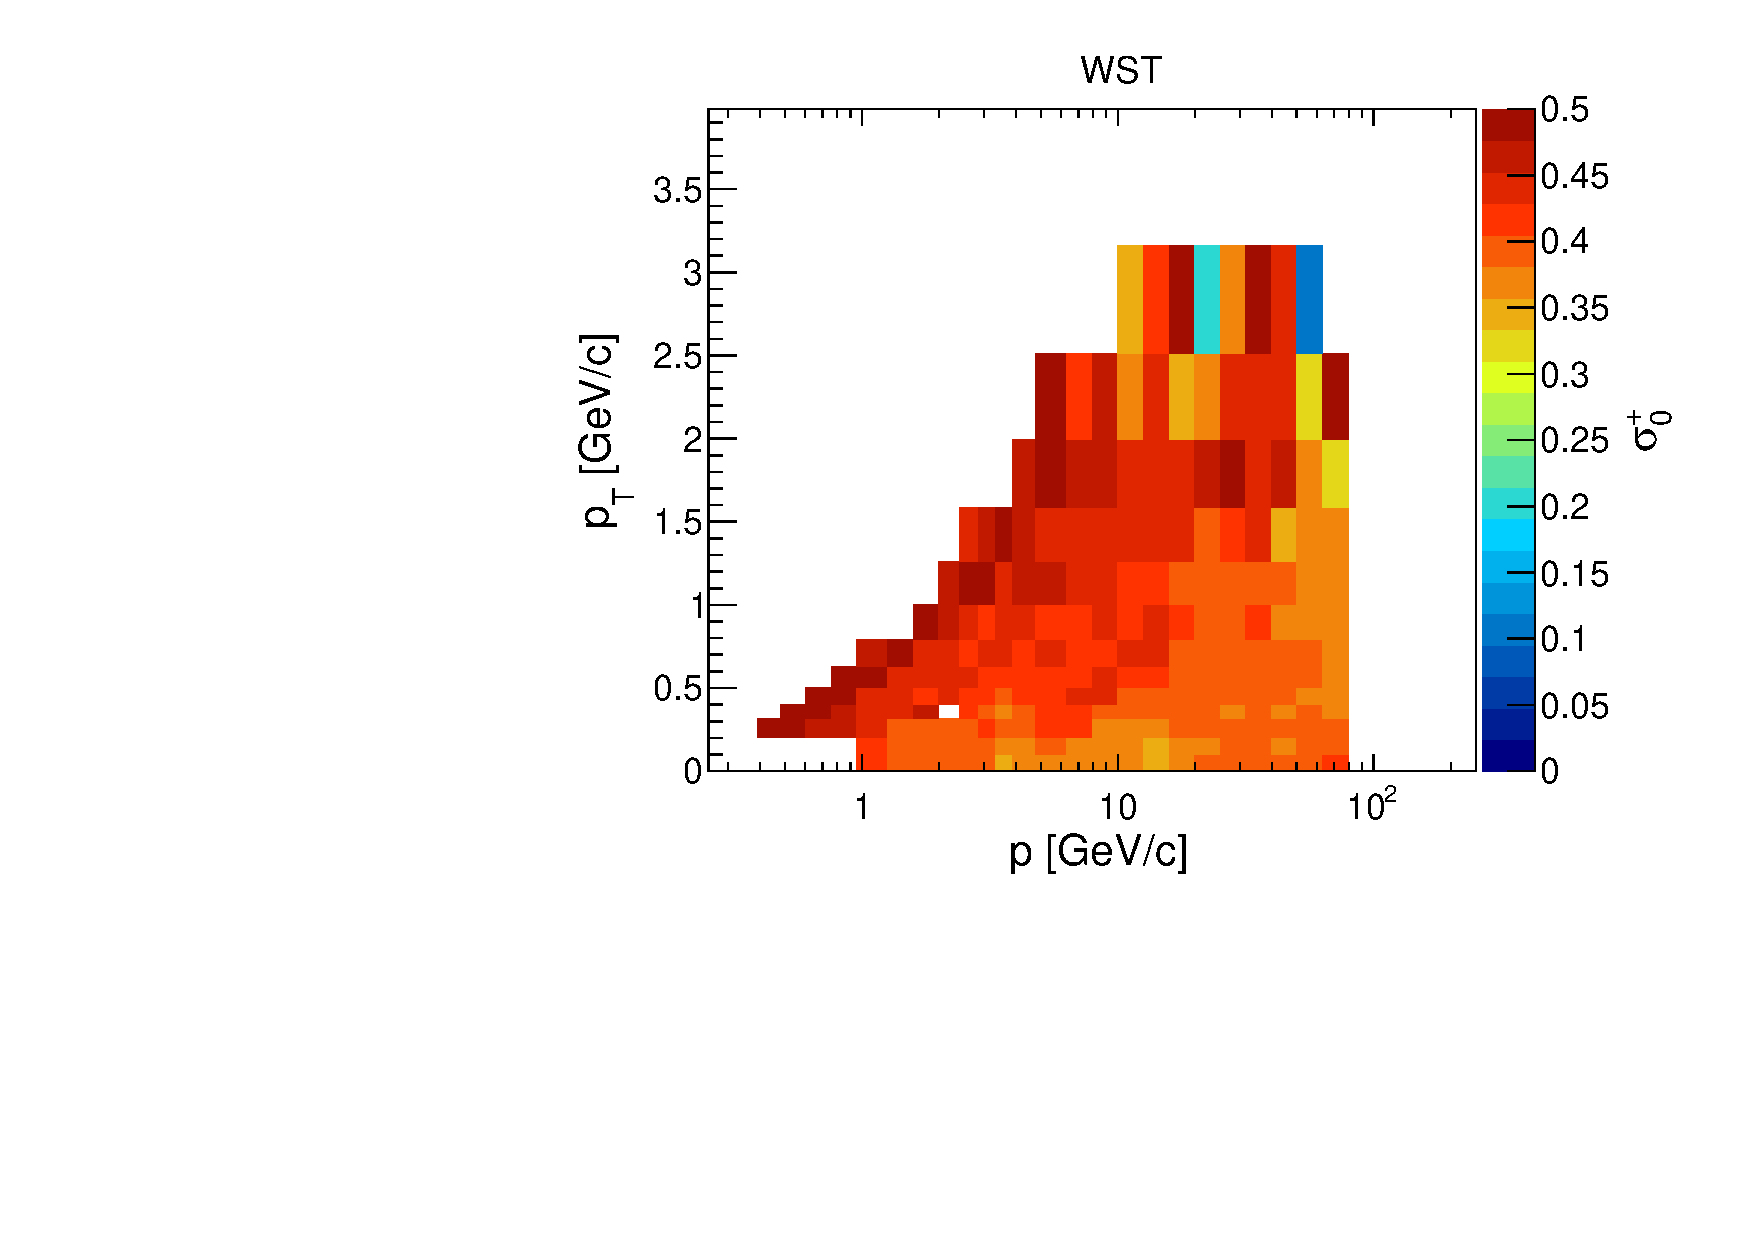
\includegraphics[clip, rviewport=0 0 1 0.94,width=0.4\textwidth]{dedx/model_350_v1_m6}
  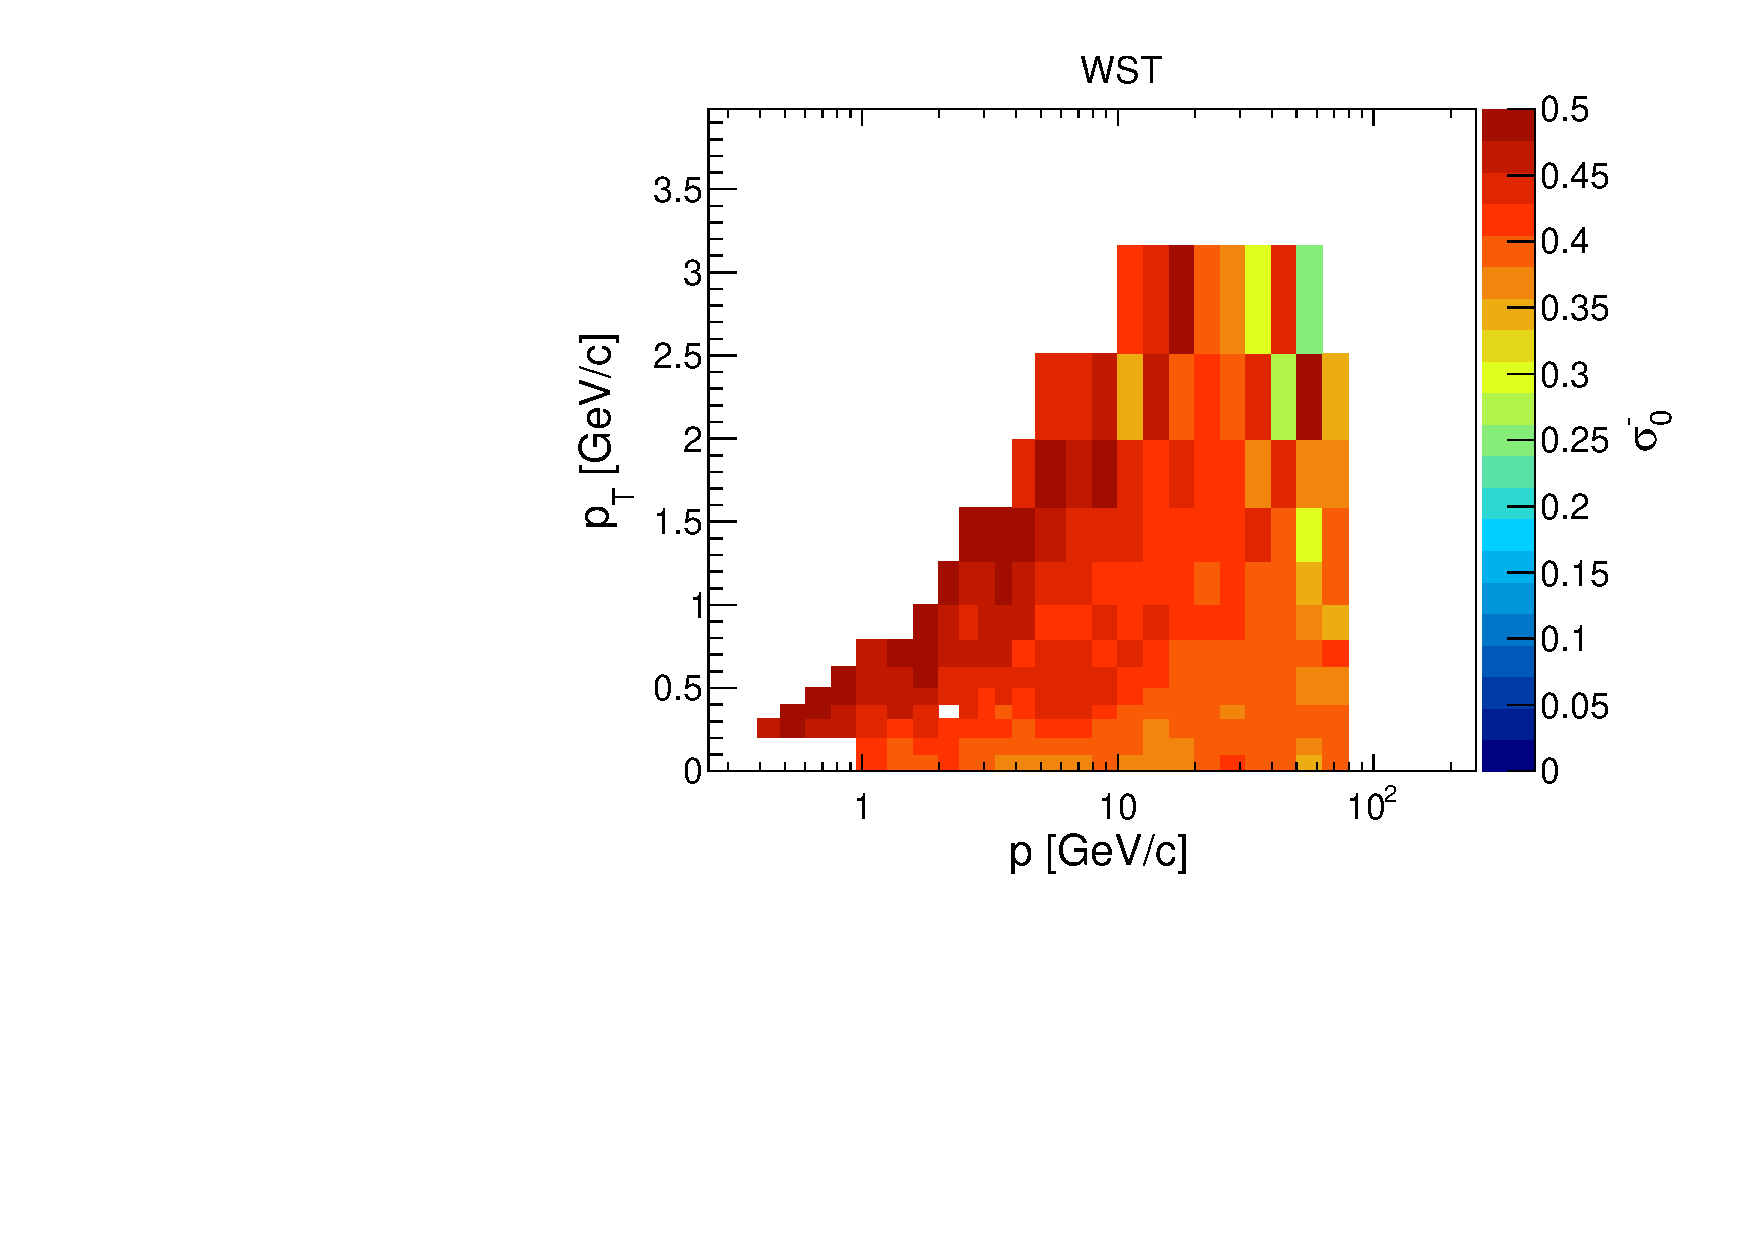
\includegraphics[clip, rviewport=0 0 1 0.94,width=0.4\textwidth]{dedx/model_350_v1_m7}

  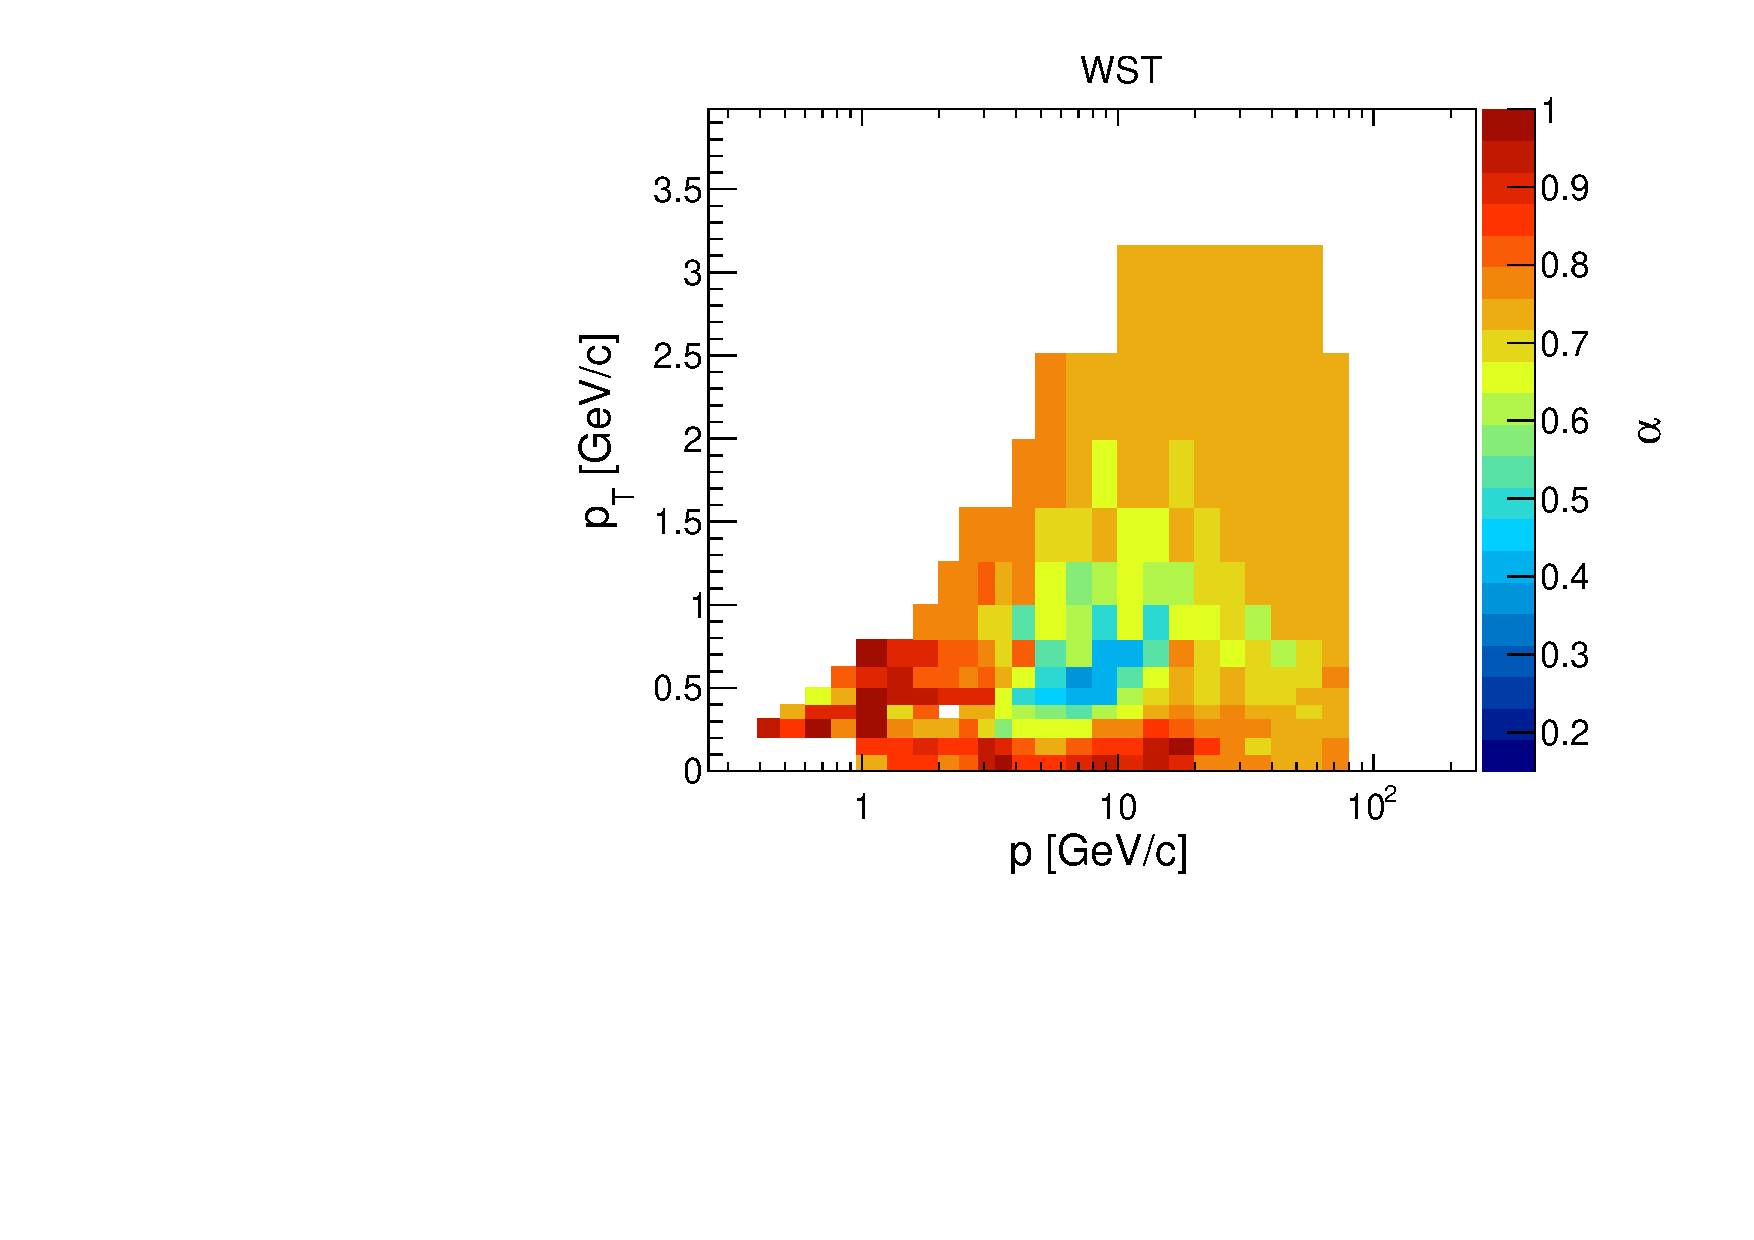
\includegraphics[clip, rviewport=0 0 1 0.94,width=0.4\textwidth]{dedx/model_350_v1_m9}
  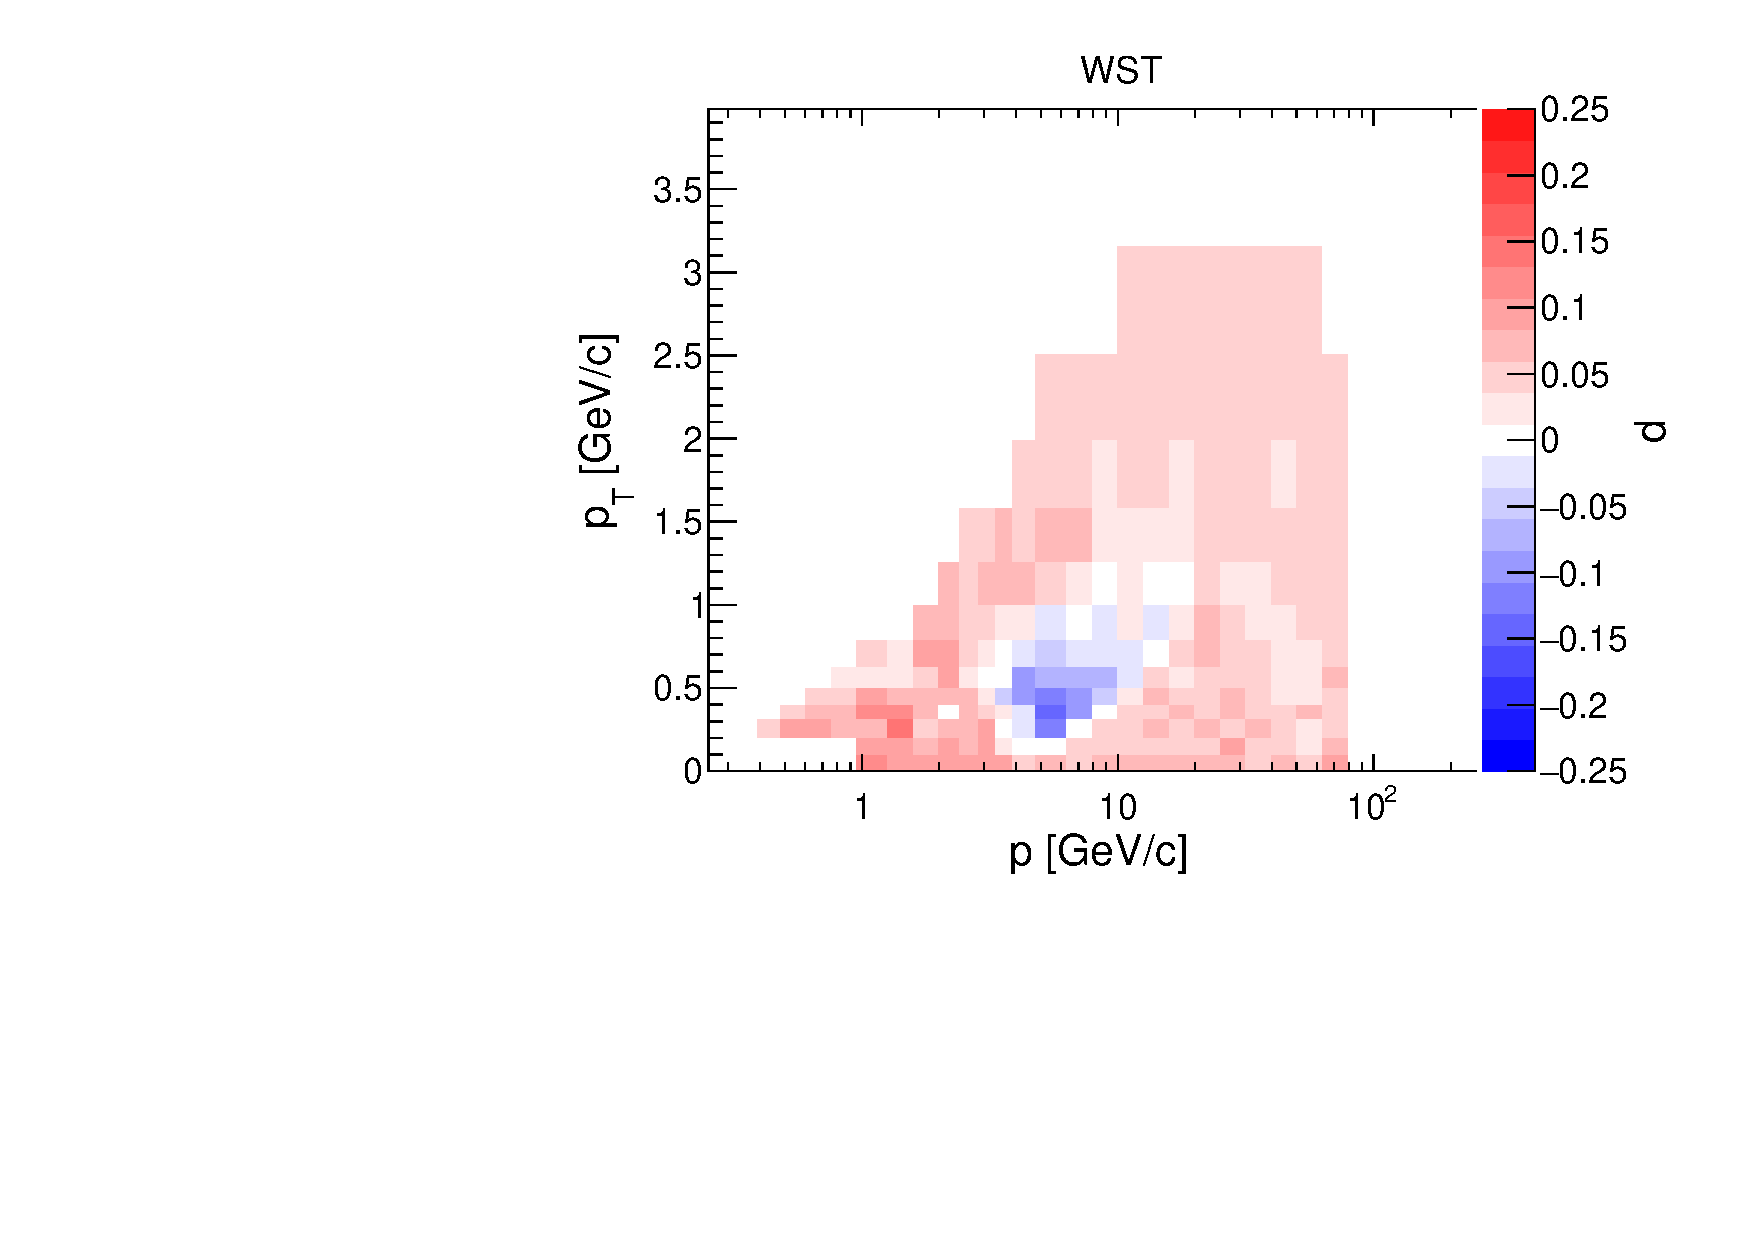
\includegraphics[clip, rviewport=0 0 1 0.94,width=0.4\textwidth]{dedx/model_350_v1_m10}
  \caption{Shape parameters obtained from the fit of the WST dataset at 350 \GeVc.}
  \label{fig:hadron:dedx:fit:shape350w}
\end{figure}

\clearpage


%%%%%%%%%% FRACTIONS %%%%%%%%%%%%%%
\begin{figure}
  \centering
  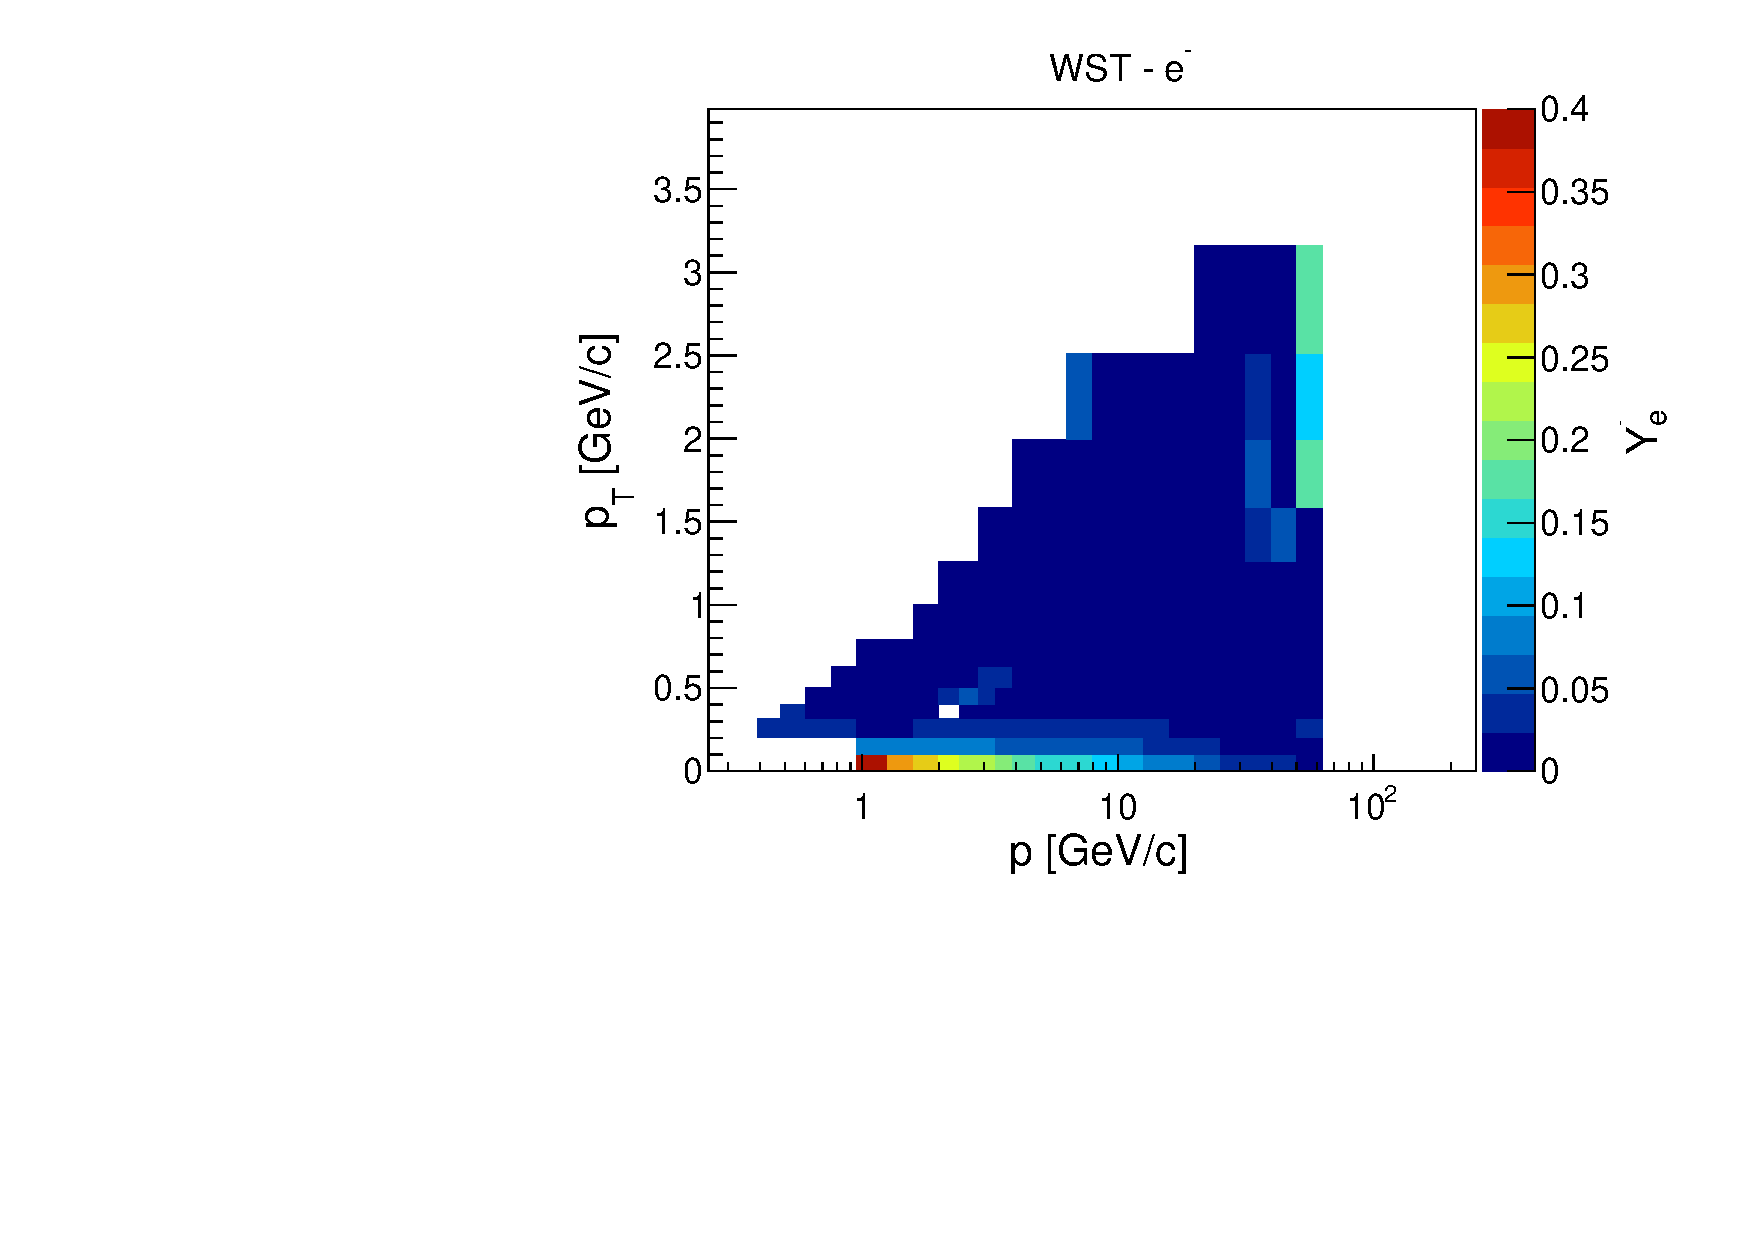
\includegraphics[clip, rviewport=0 0.13 1 0.94,width=0.4\textwidth]{dedx/fraction_158_fl0_v1_c0_p0}
  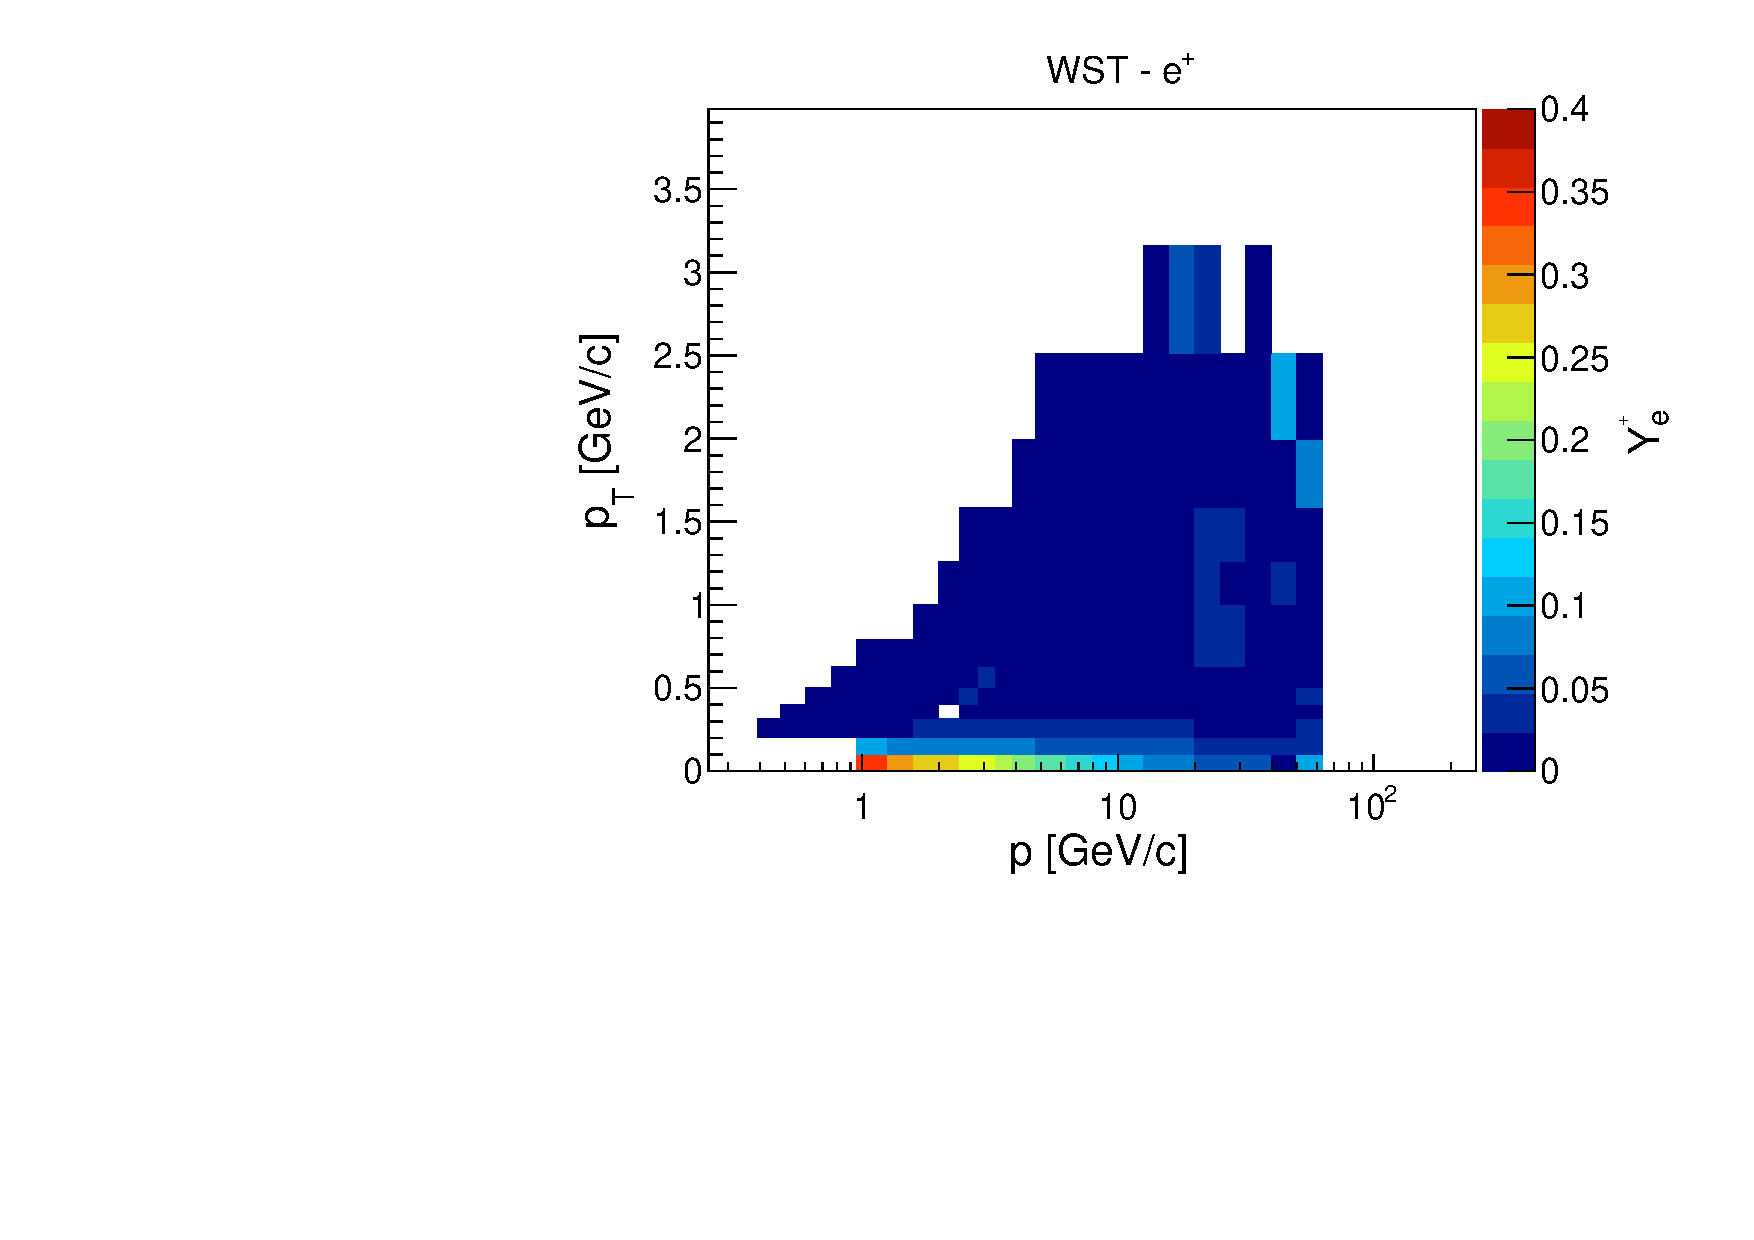
\includegraphics[clip, rviewport=0 0.13 1 0.94,width=0.4\textwidth]{dedx/fraction_158_fl0_v1_c1_p0}

  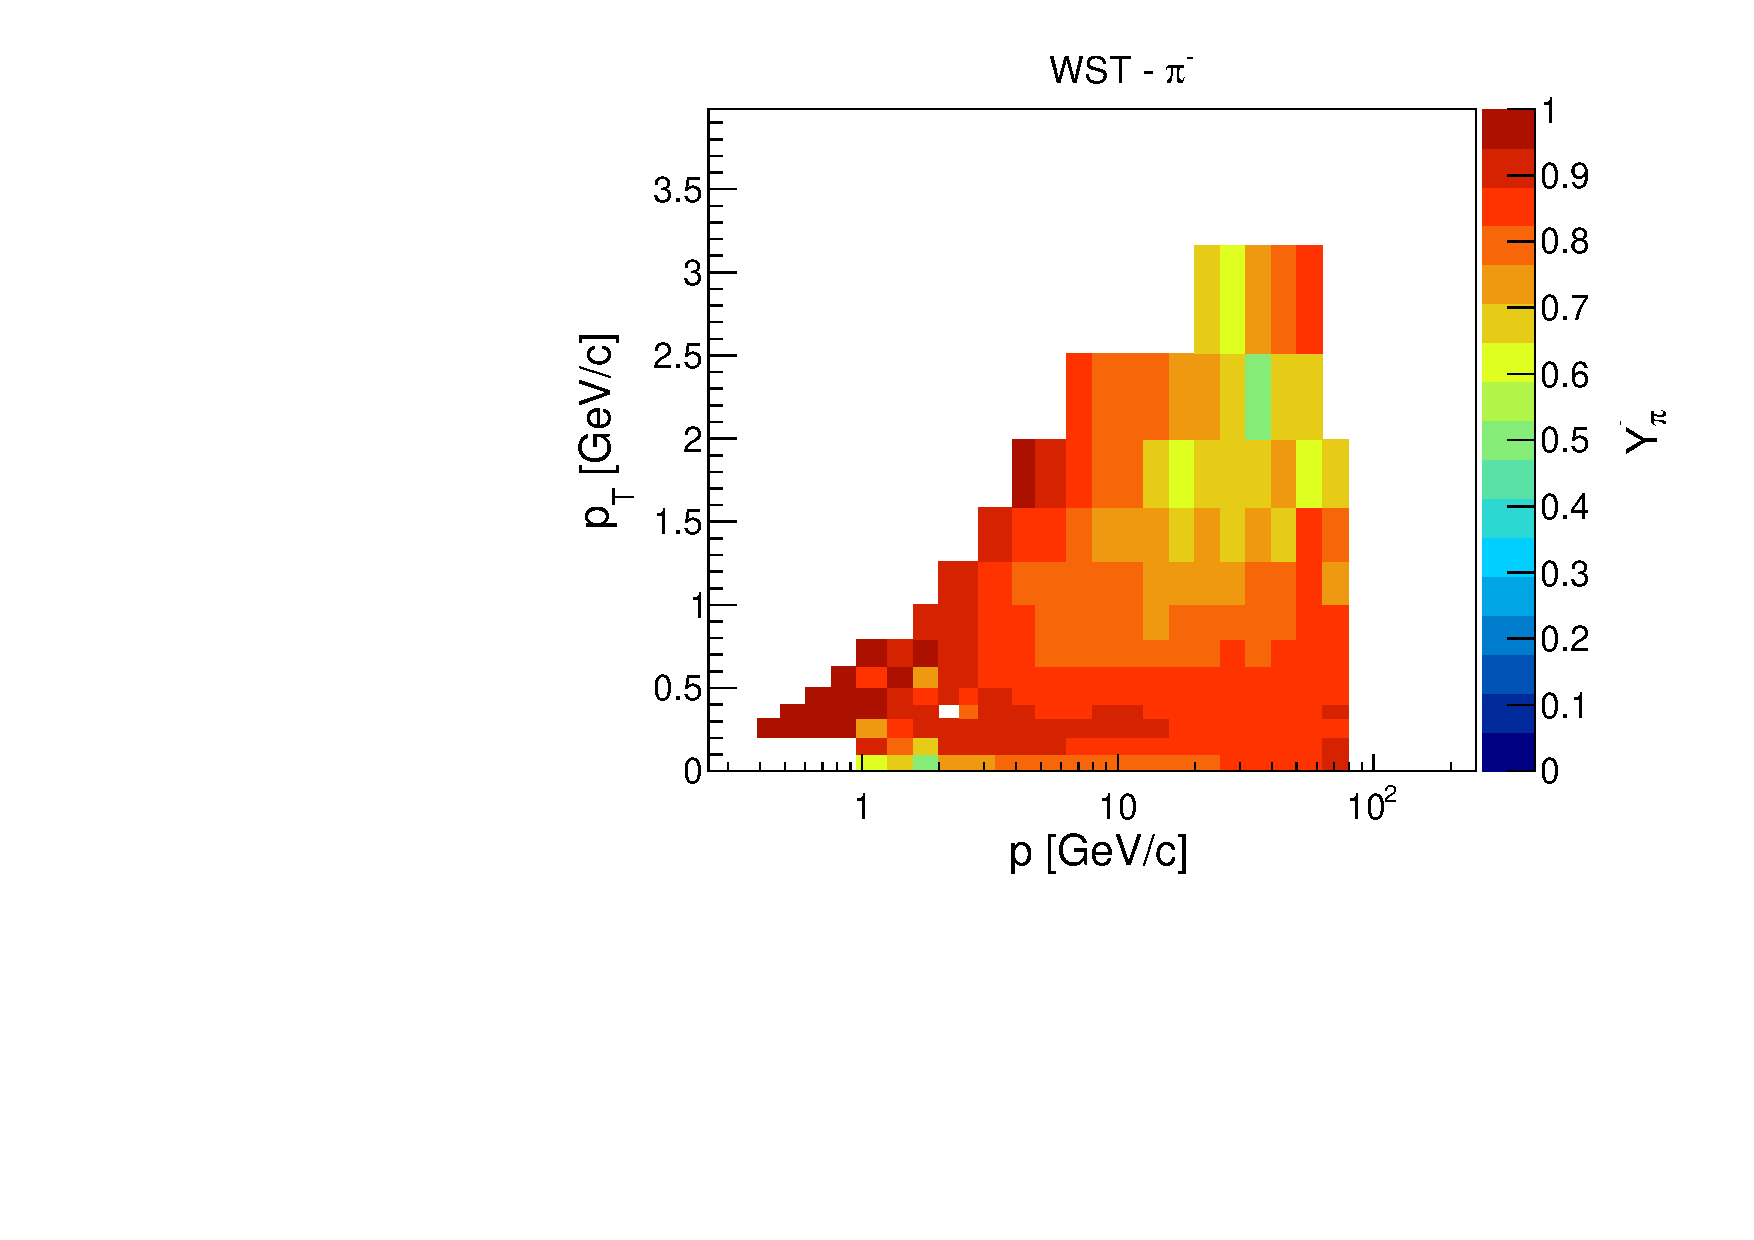
\includegraphics[clip, rviewport=0 0.13 1 0.94,width=0.4\textwidth]{dedx/fraction_158_fl0_v1_c0_p1}
  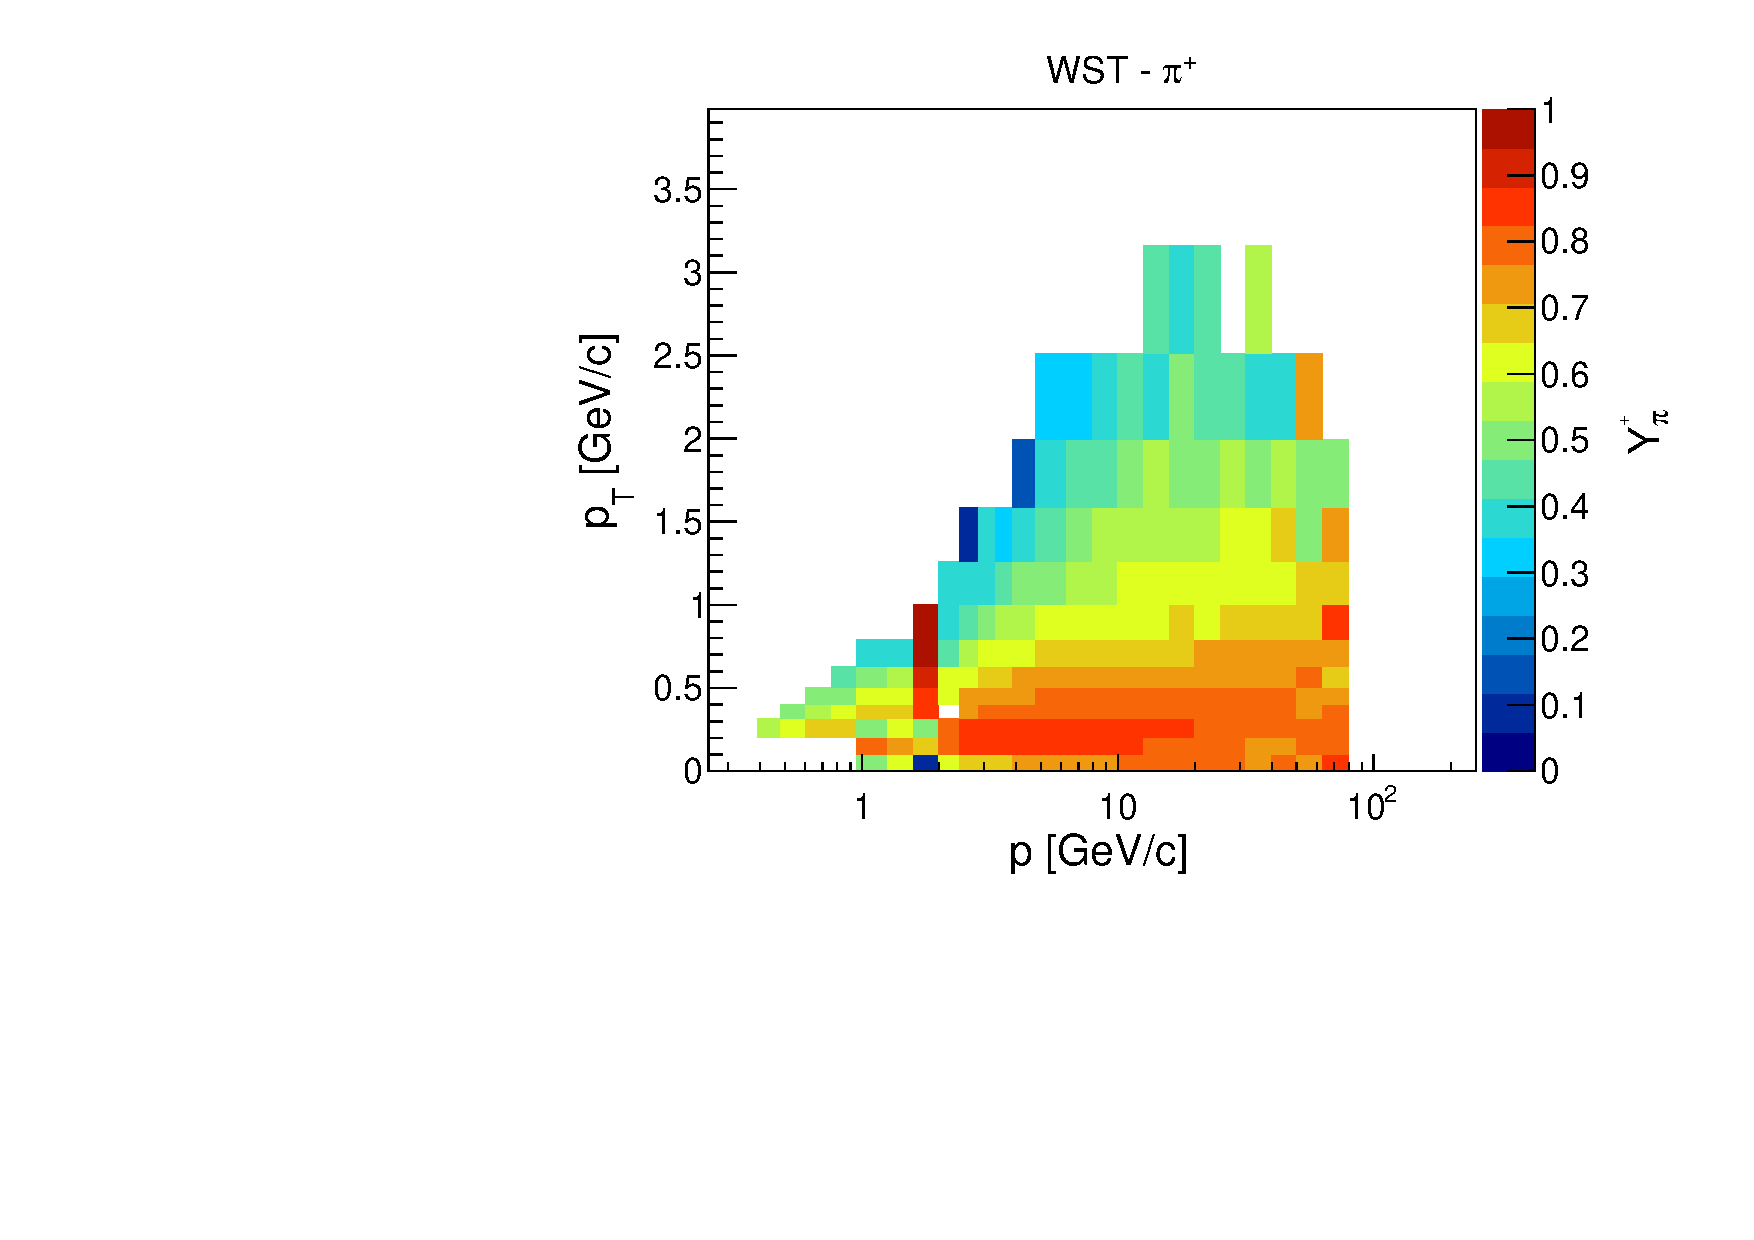
\includegraphics[clip, rviewport=0 0.13 1 0.94,width=0.4\textwidth]{dedx/fraction_158_fl0_v1_c1_p1}

  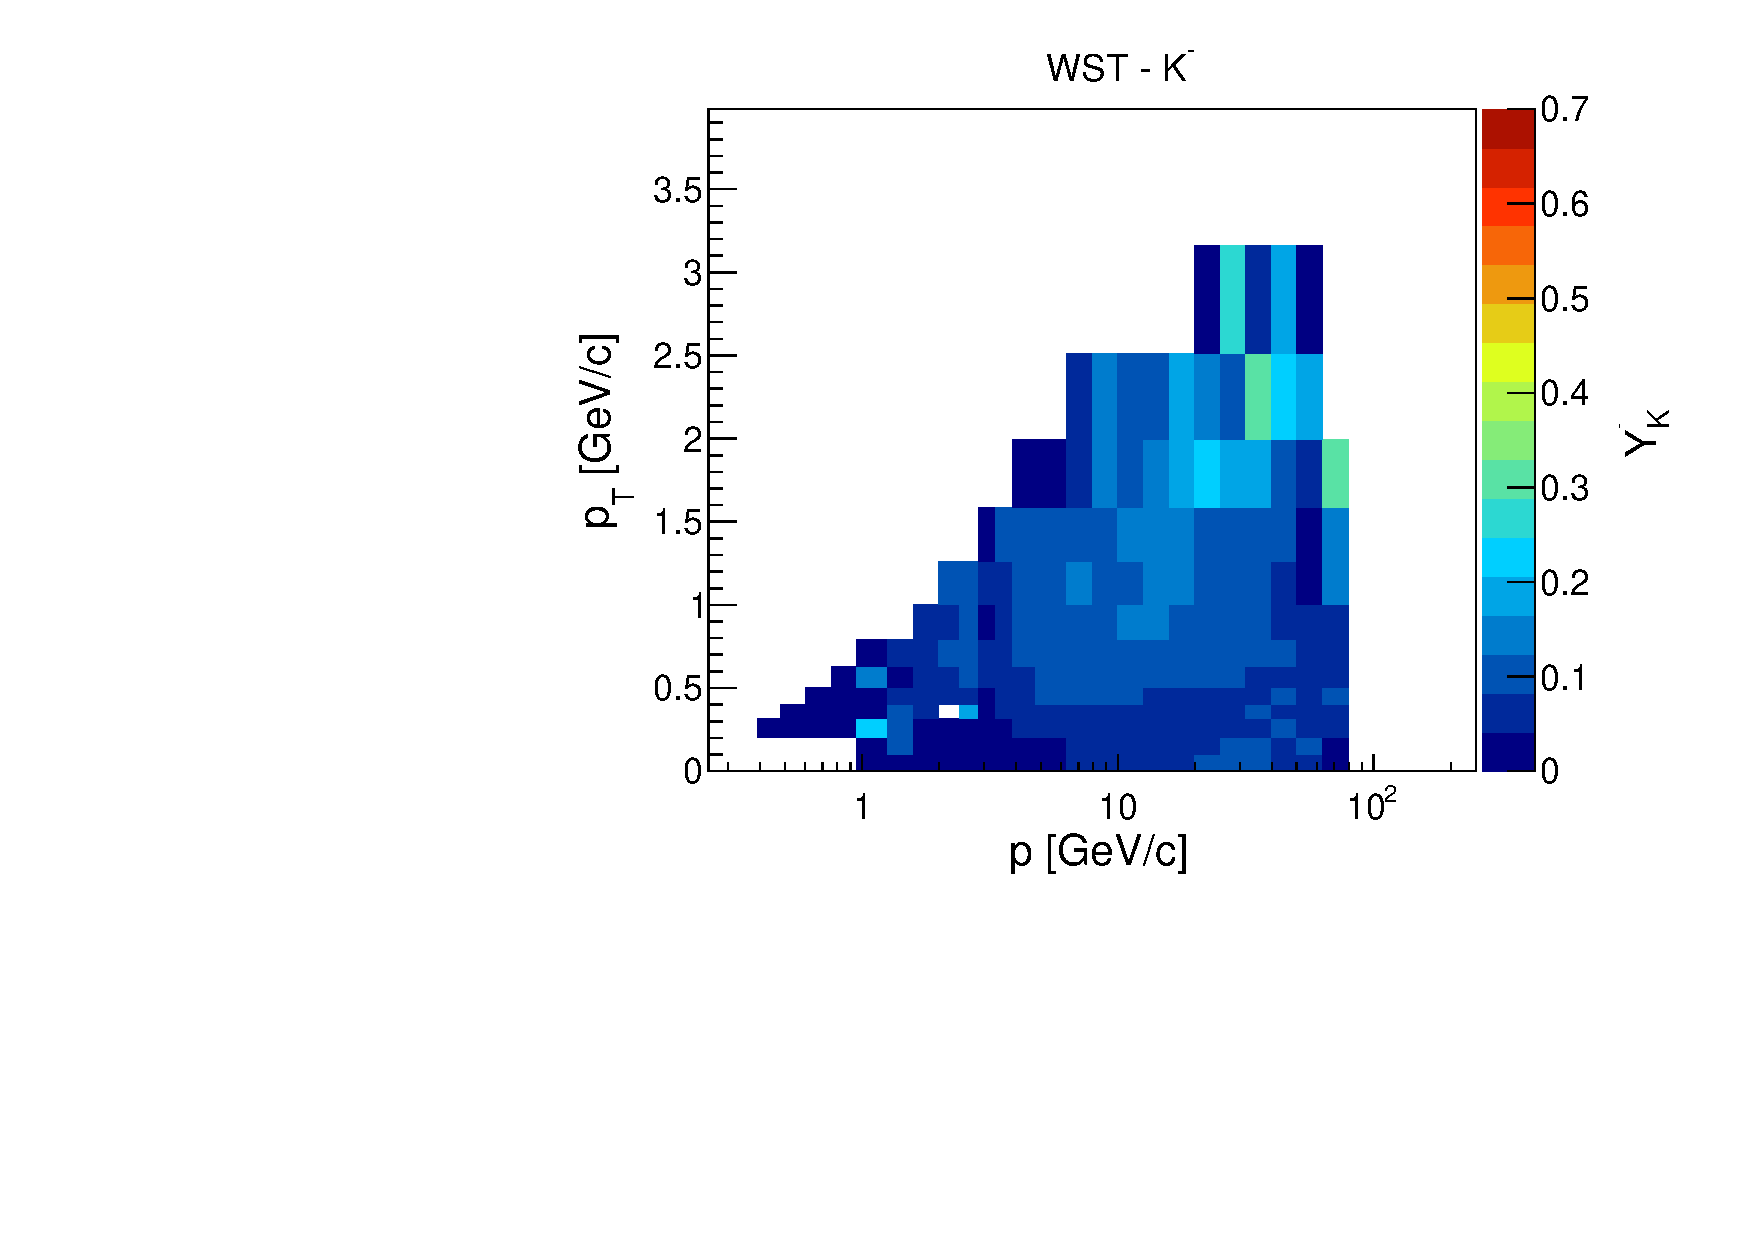
\includegraphics[clip, rviewport=0 0.13 1 0.94,width=0.4\textwidth]{dedx/fraction_158_fl0_v1_c0_p2}
  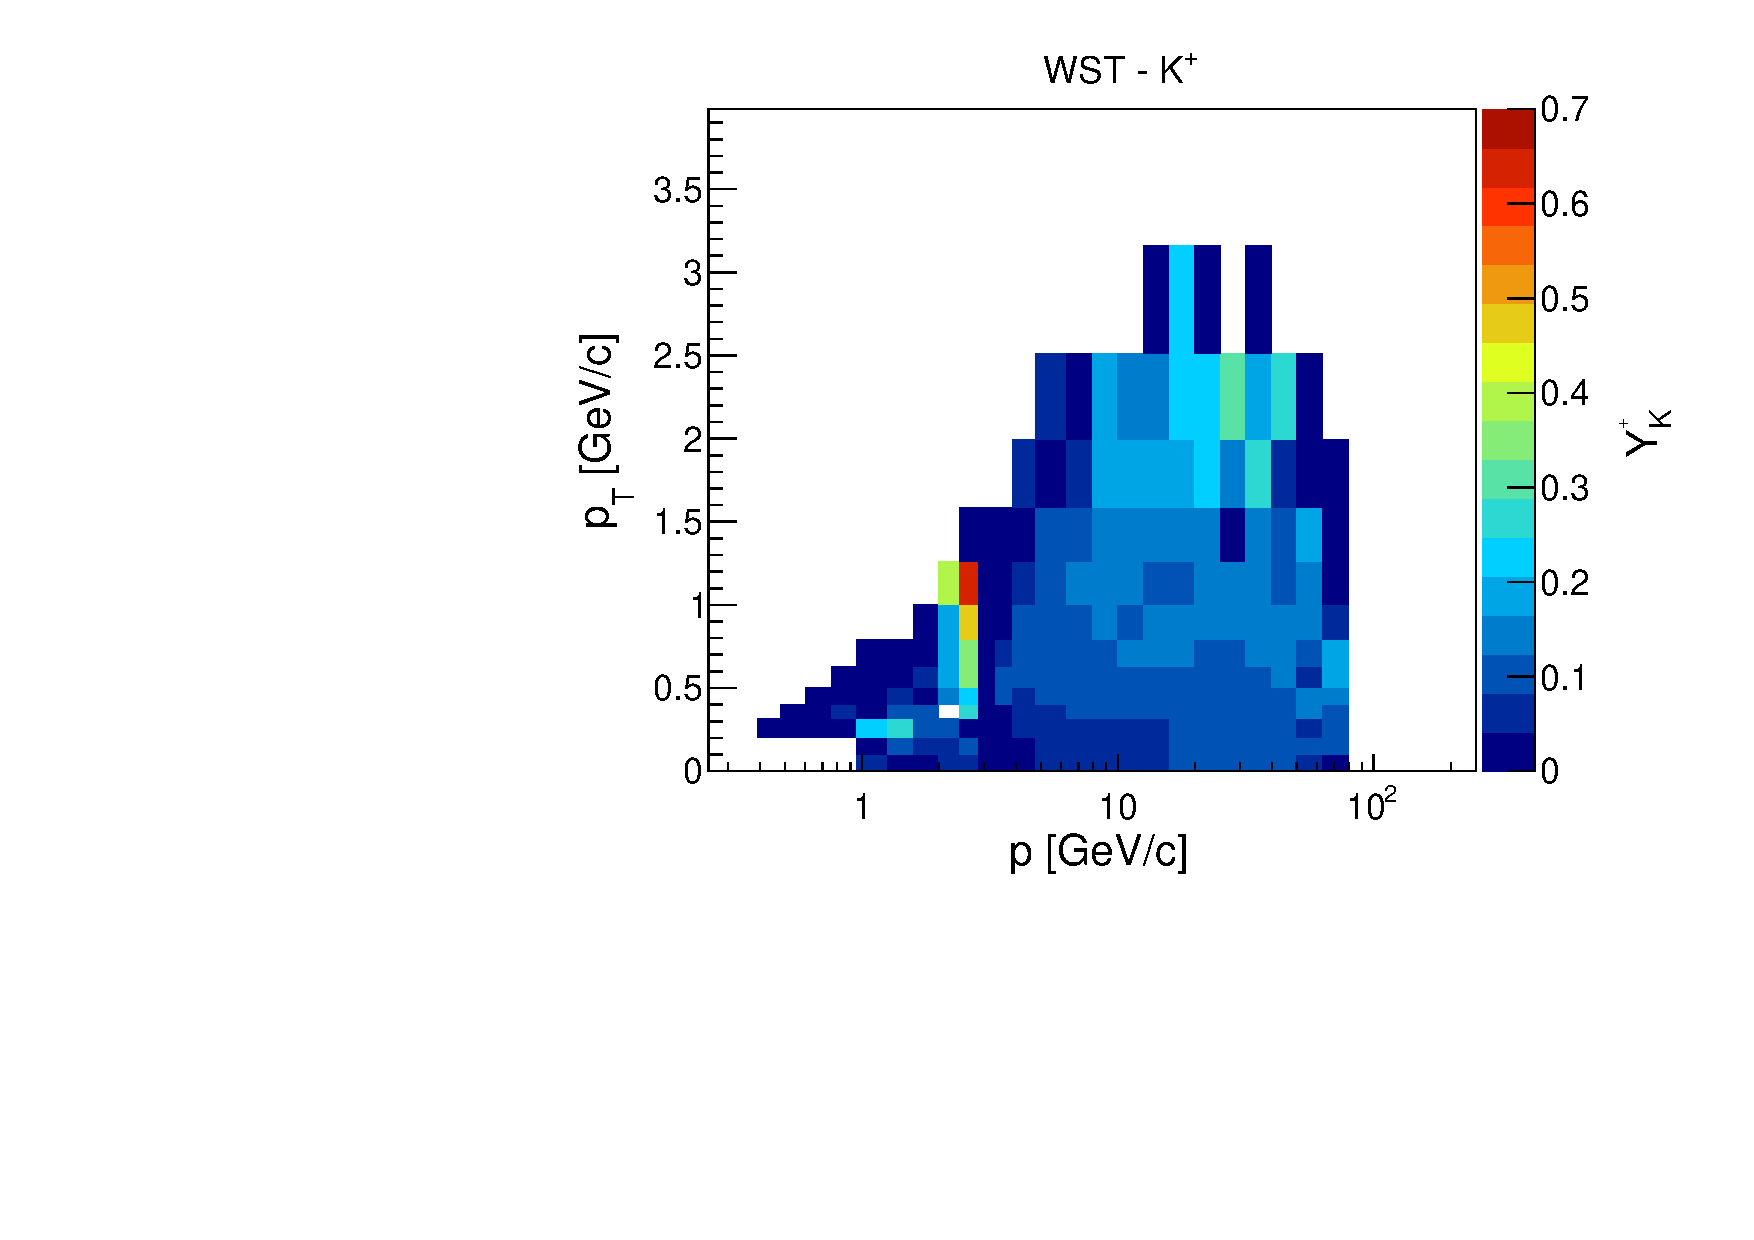
\includegraphics[clip, rviewport=0 0.13 1 0.94,width=0.4\textwidth]{dedx/fraction_158_fl0_v1_c1_p2}


  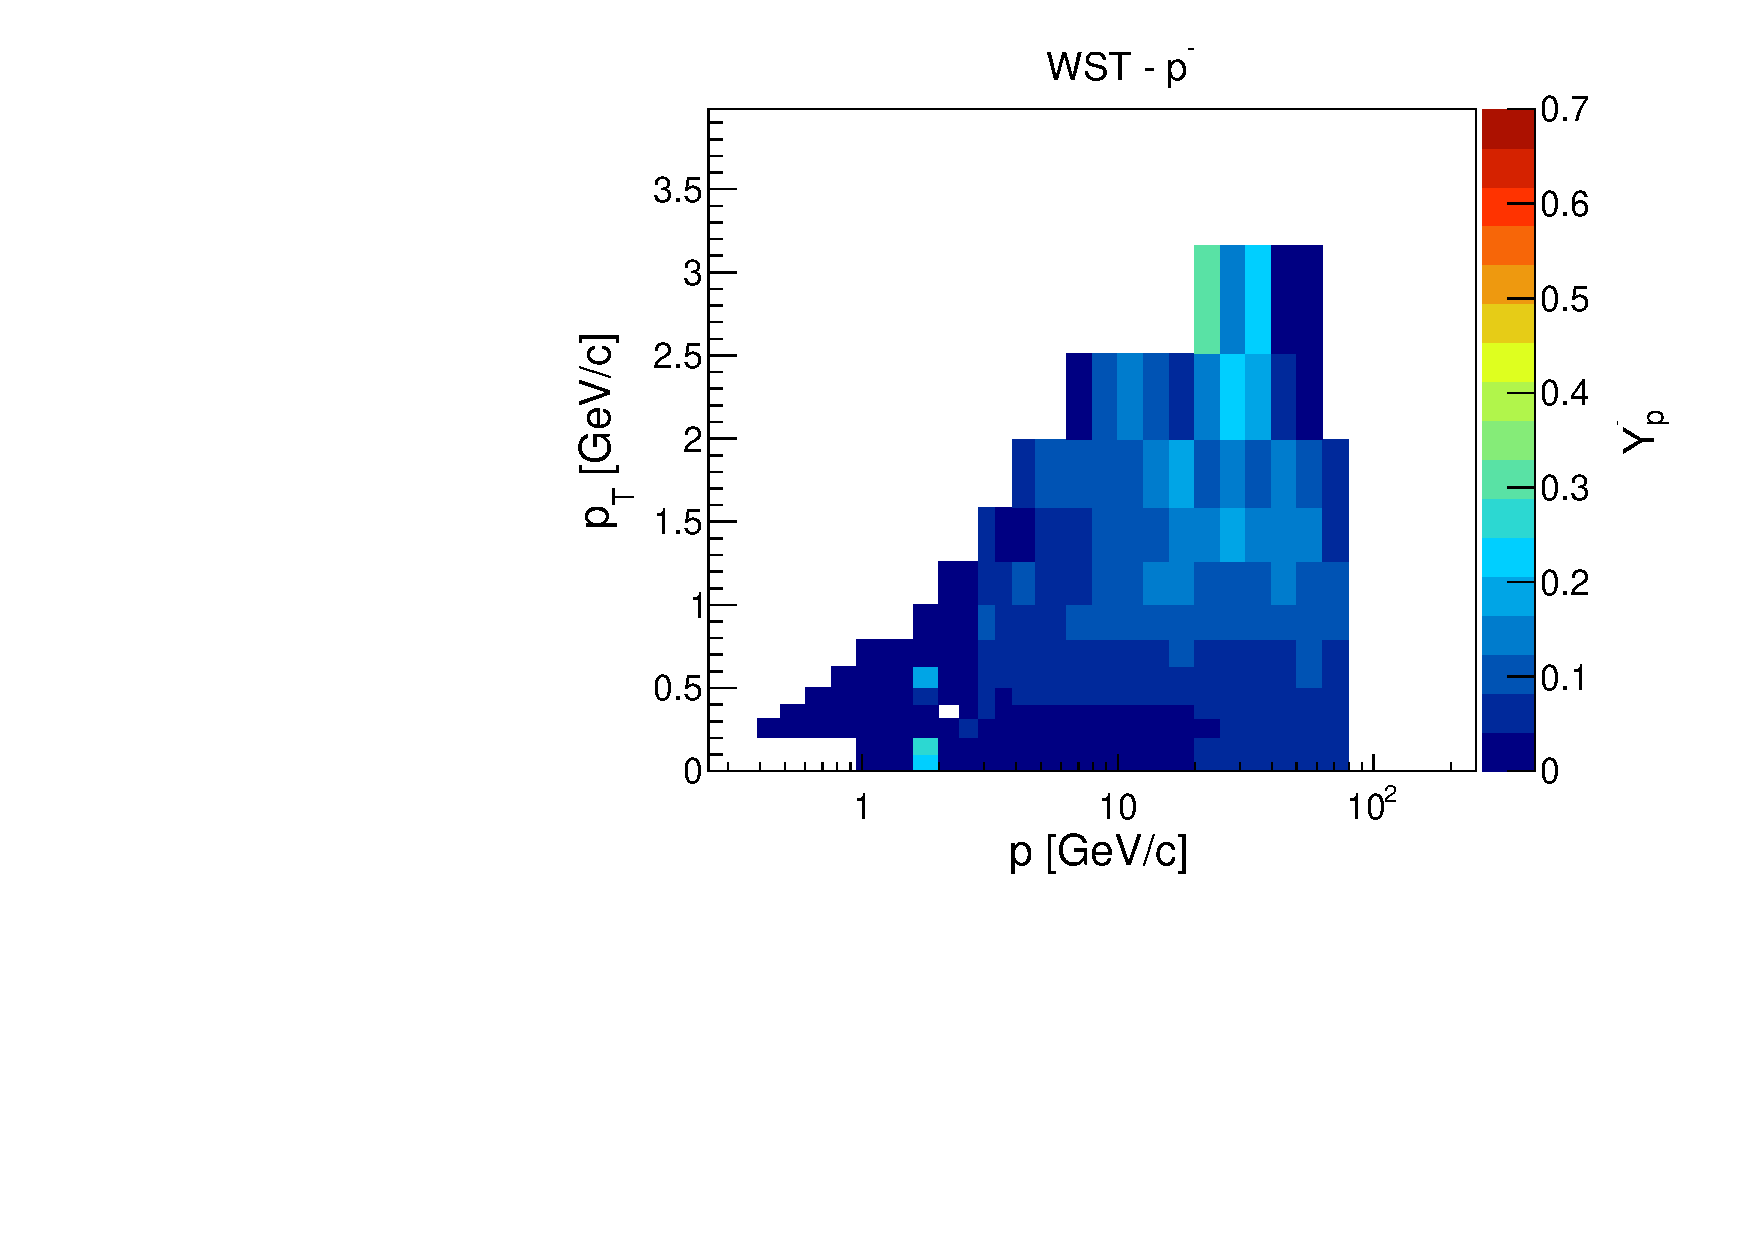
\includegraphics[clip, rviewport=0 0.13 1 0.94,width=0.4\textwidth]{dedx/fraction_158_fl0_v1_c0_p3}
  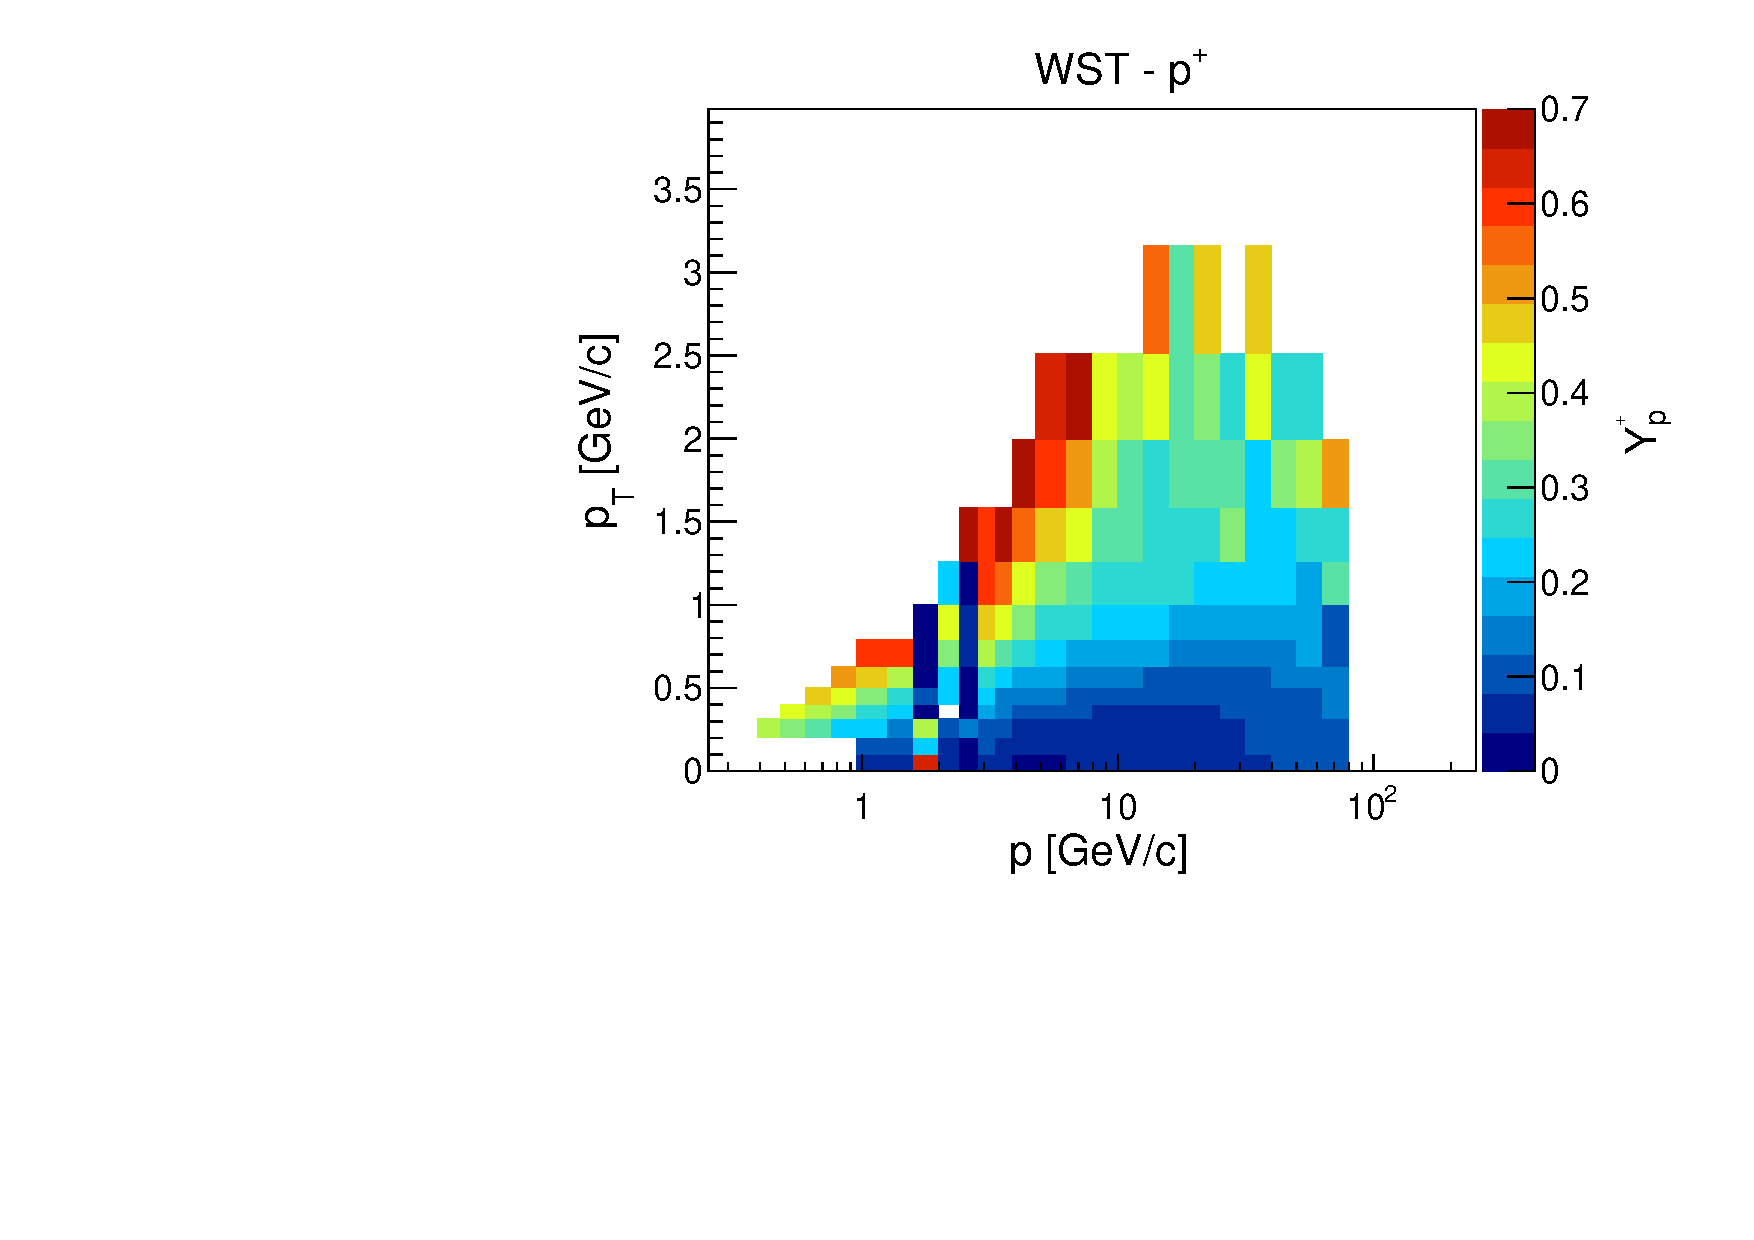
\includegraphics[clip, rviewport=0 0.13 1 0.94,width=0.4\textwidth]{dedx/fraction_158_fl0_v1_c1_p3}

  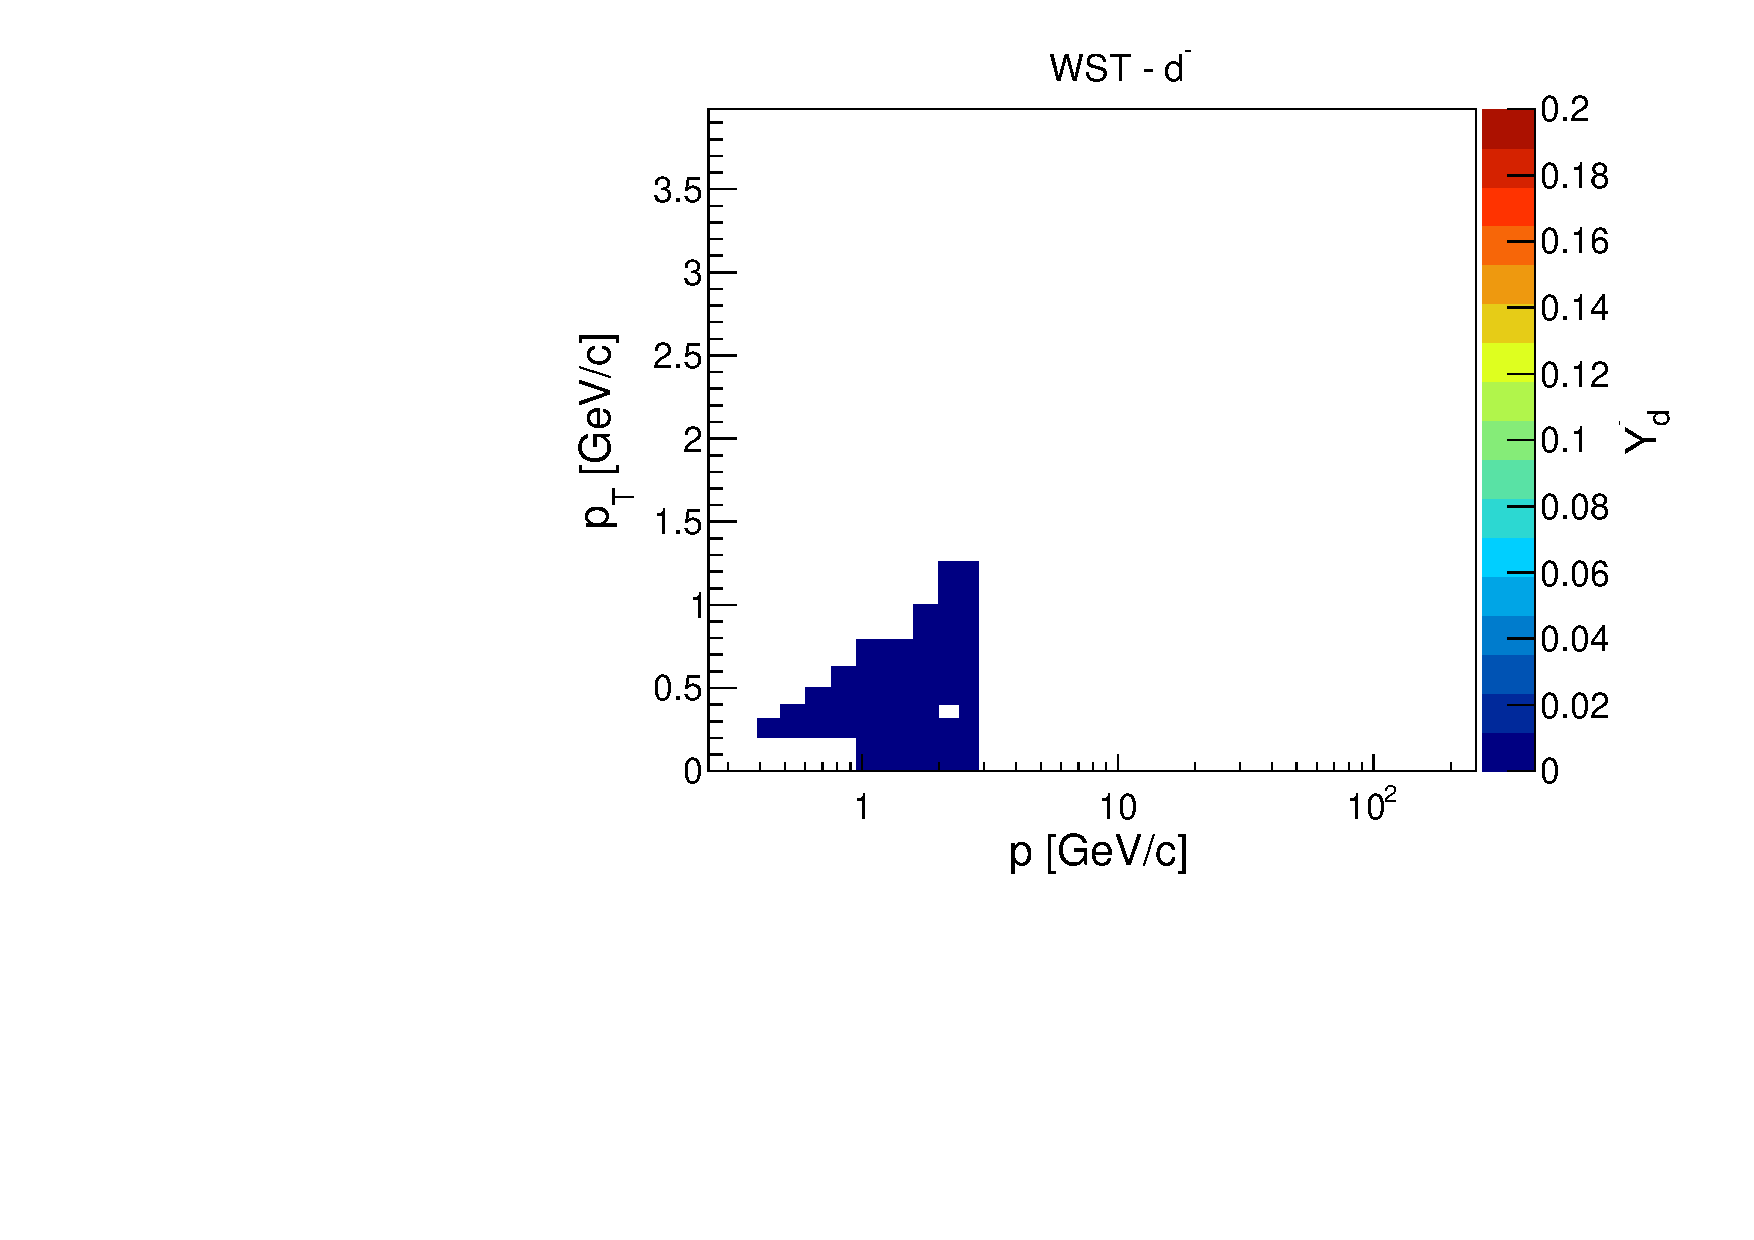
\includegraphics[clip, rviewport=0 0 1 0.94,width=0.4\textwidth]{dedx/fraction_158_fl0_v1_c0_p4}
  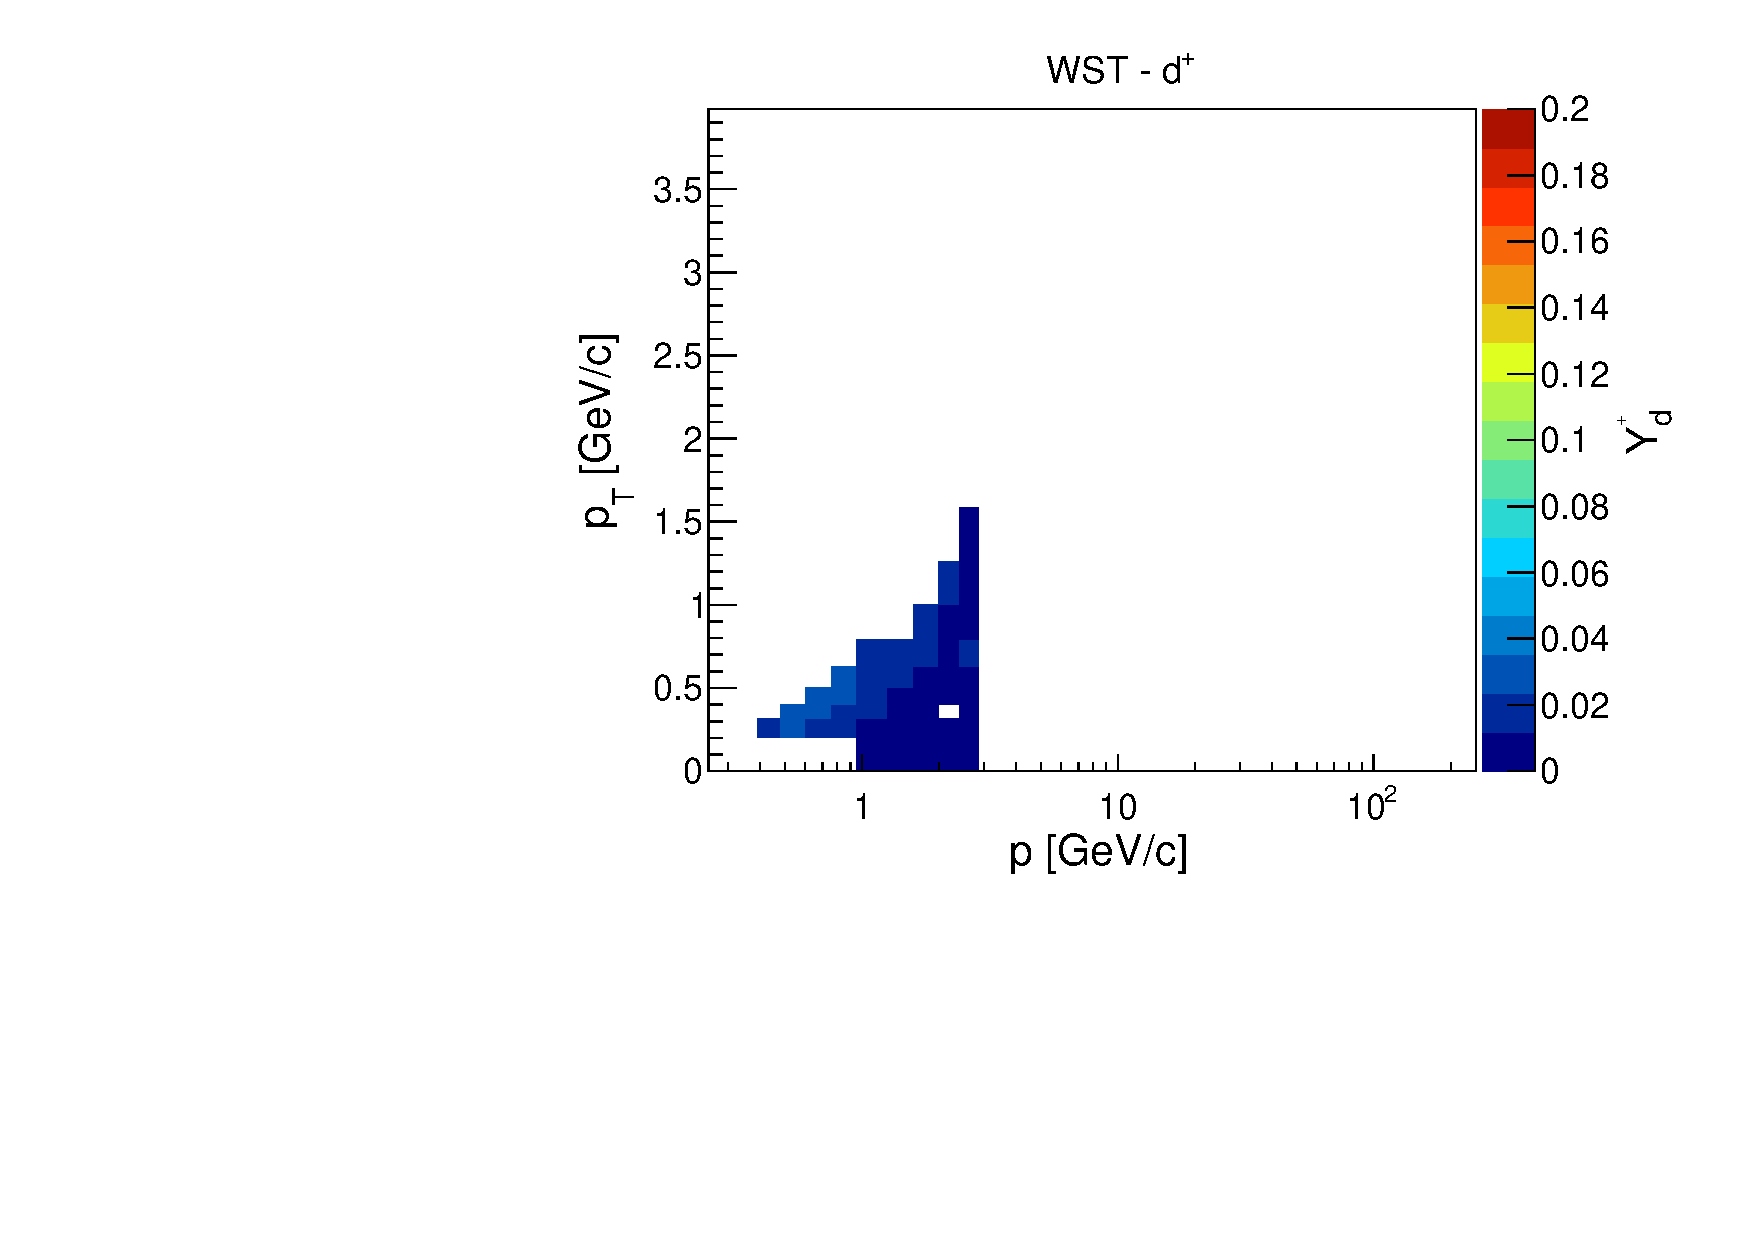
\includegraphics[clip, rviewport=0 0 1 0.94,width=0.4\textwidth]{dedx/fraction_158_fl0_v1_c1_p4}

  \caption{Particle fractions obtained from the fit of the WST dataset at 158 \GeVc.}
  \label{fig:hadron:dedx:fit:frac158w}
\end{figure}


%%%%%%%%%% FRACTIONS %%%%%%%%%%%%%%
\begin{figure}
  \centering
  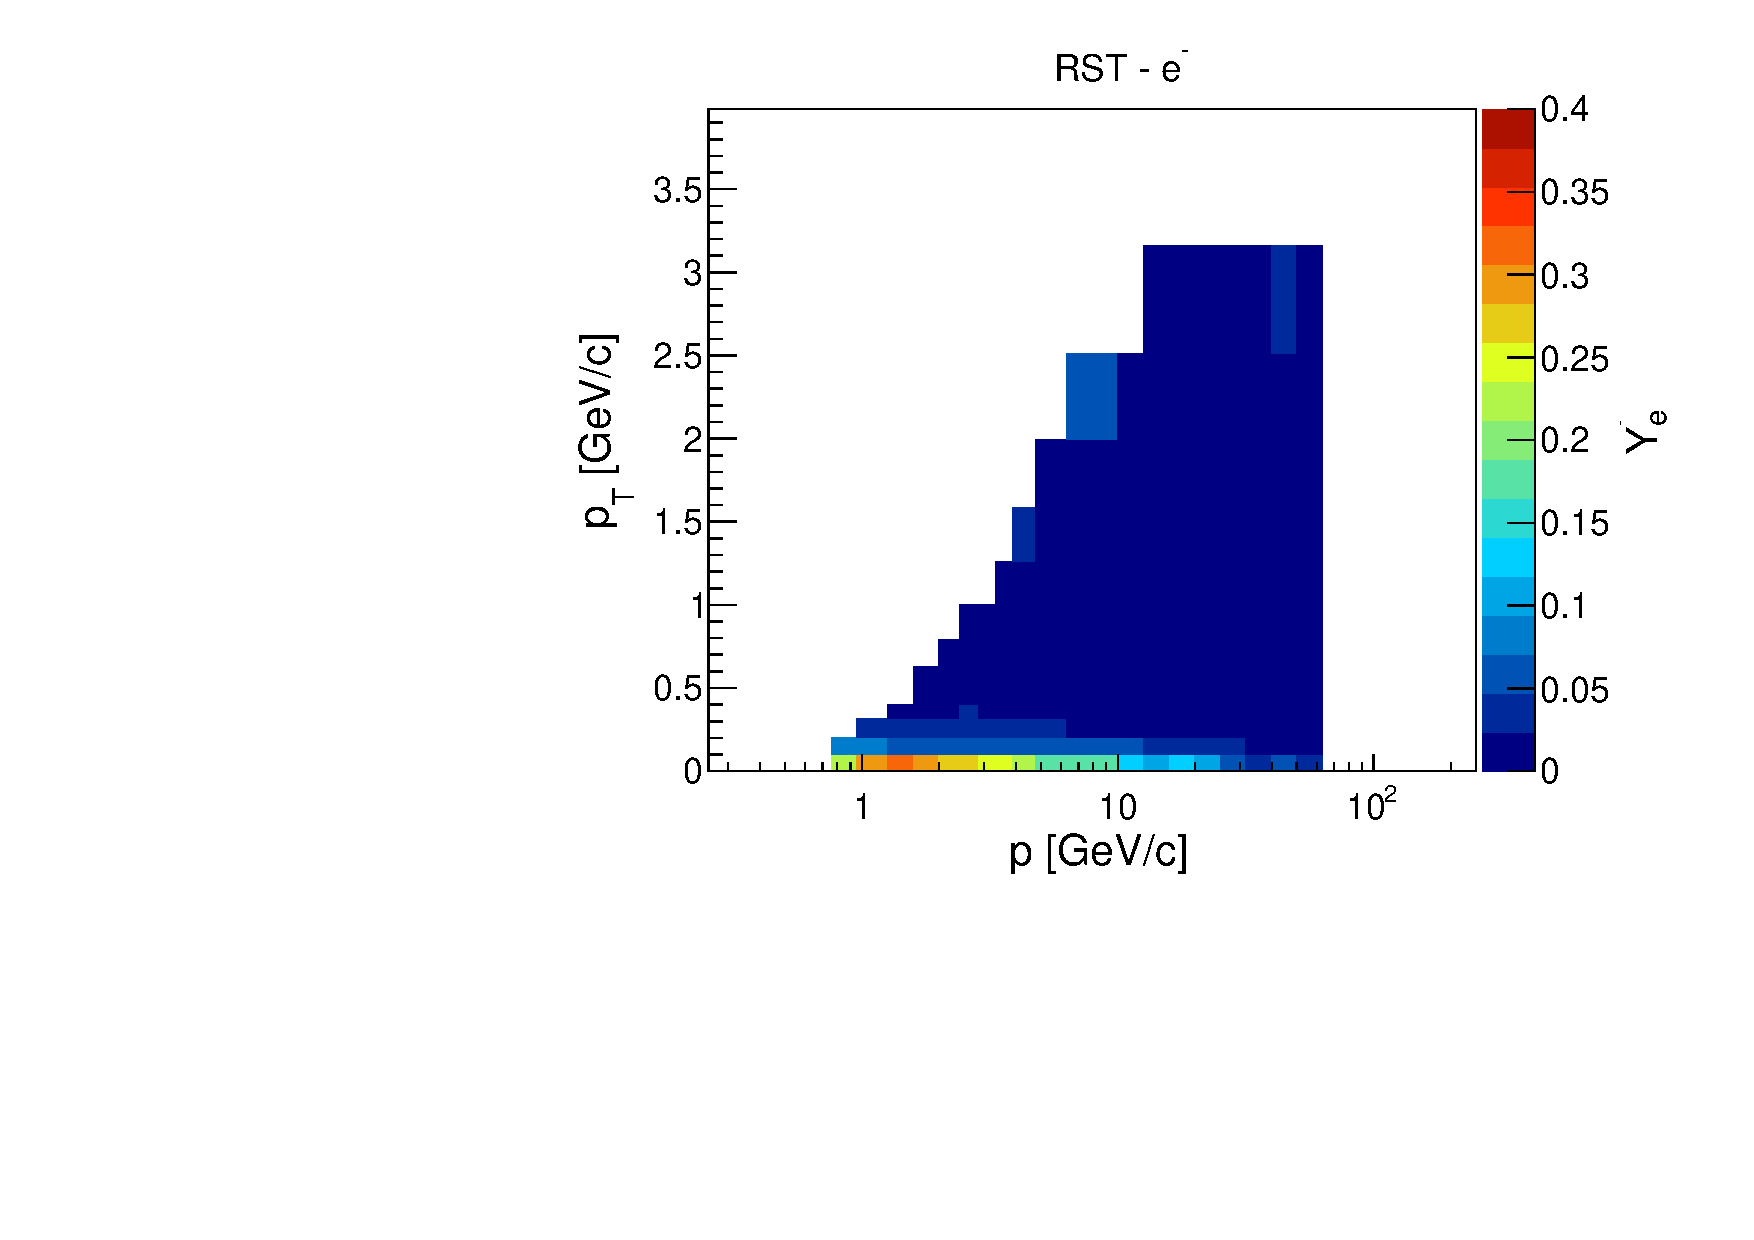
\includegraphics[clip, rviewport=0 0.13 1 0.94,width=0.4\textwidth]{dedx/fraction_350_fl0_v0_c0_p0}
  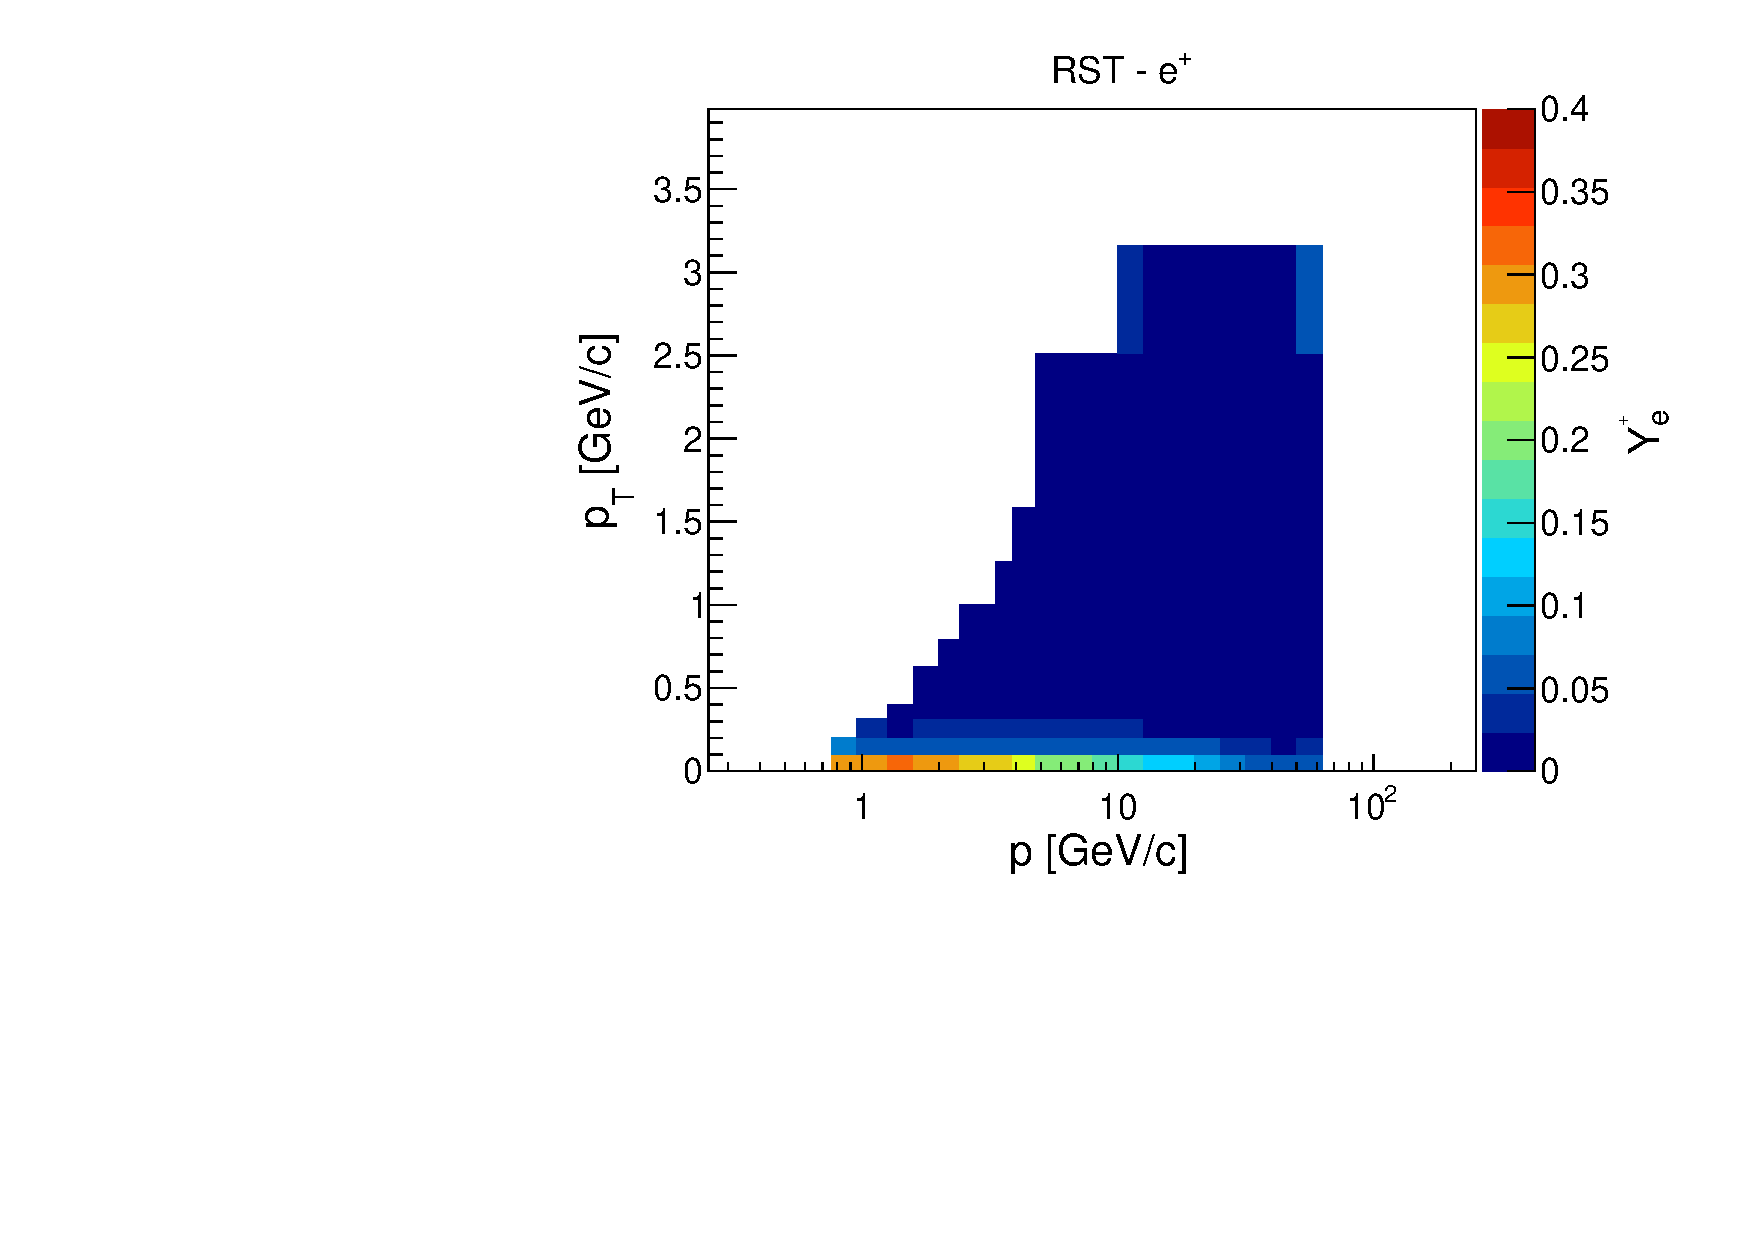
\includegraphics[clip, rviewport=0 0.13 1 0.94,width=0.4\textwidth]{dedx/fraction_350_fl0_v0_c1_p0}

  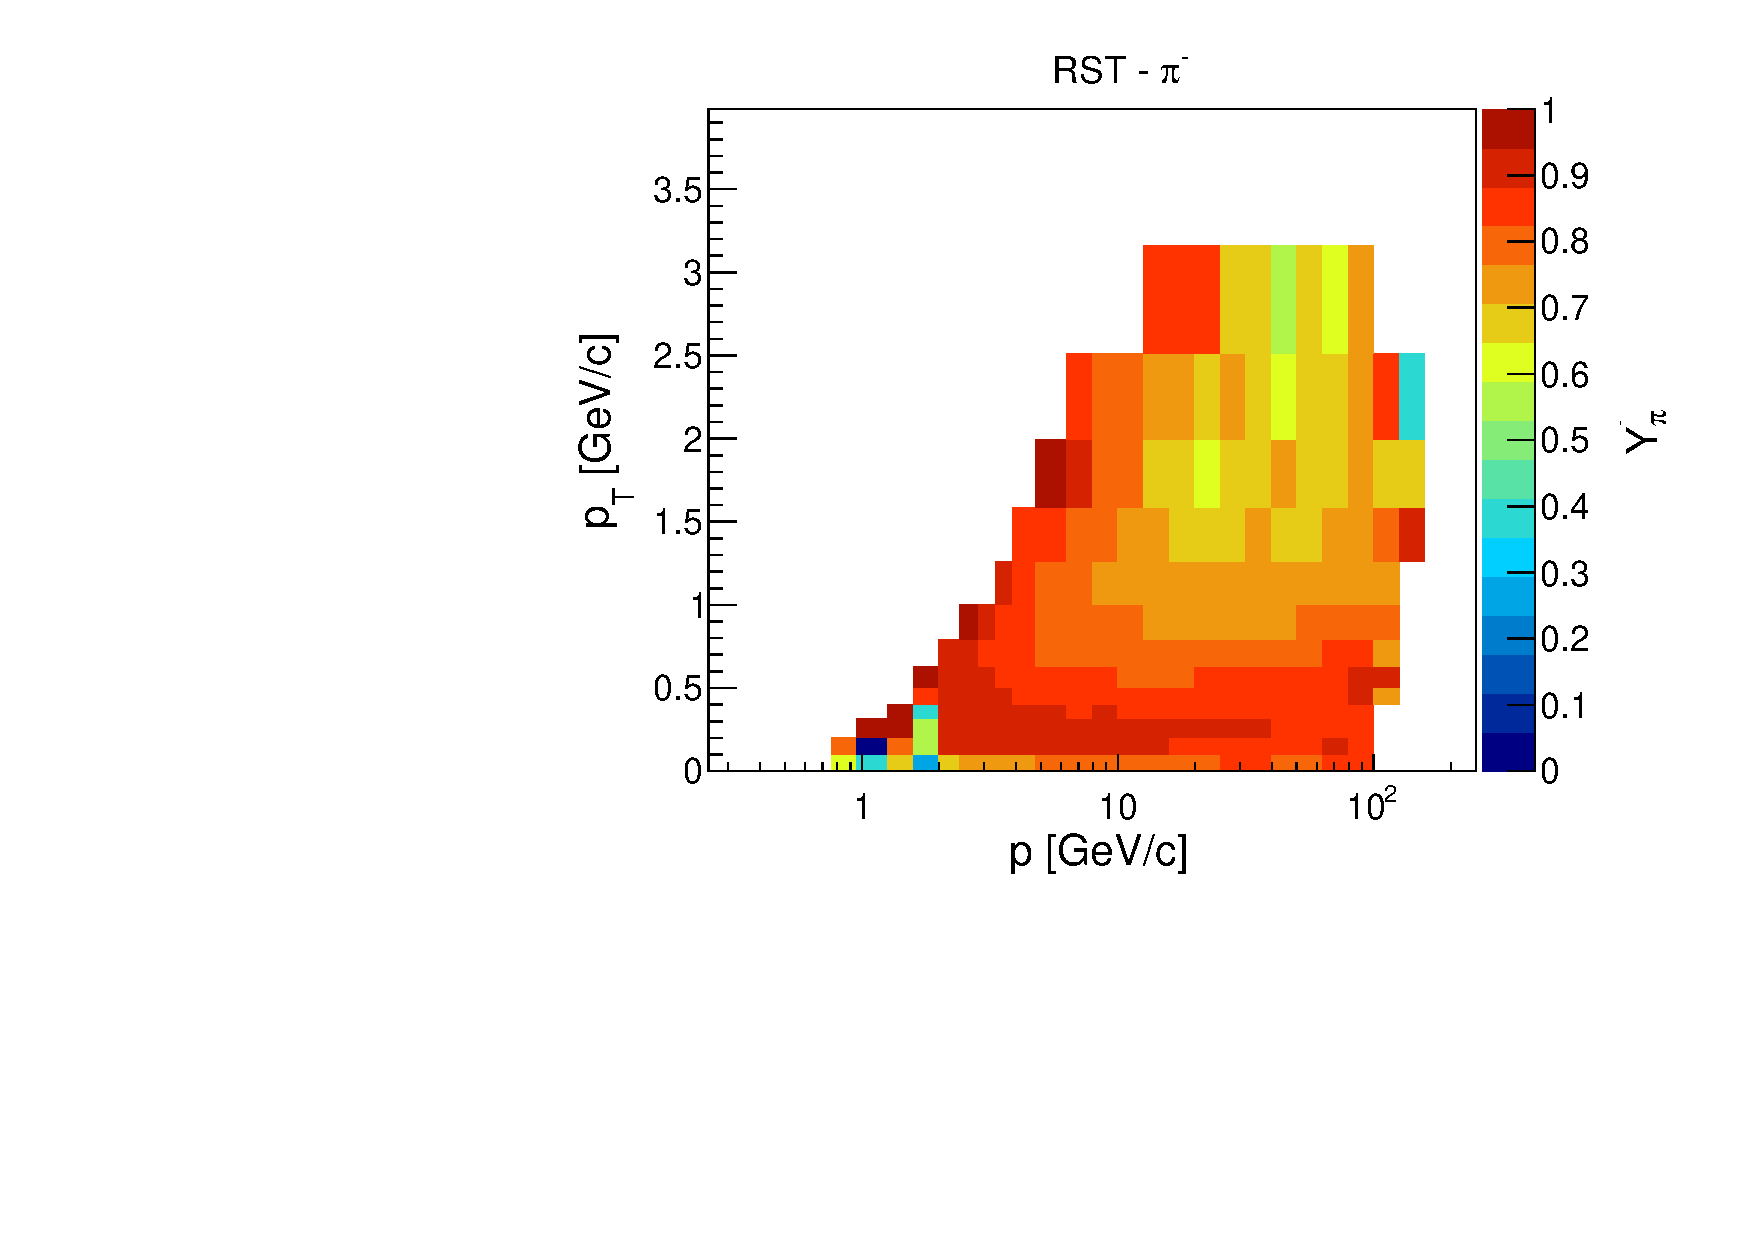
\includegraphics[clip, rviewport=0 0.13 1 0.94,width=0.4\textwidth]{dedx/fraction_350_fl0_v0_c0_p1}
  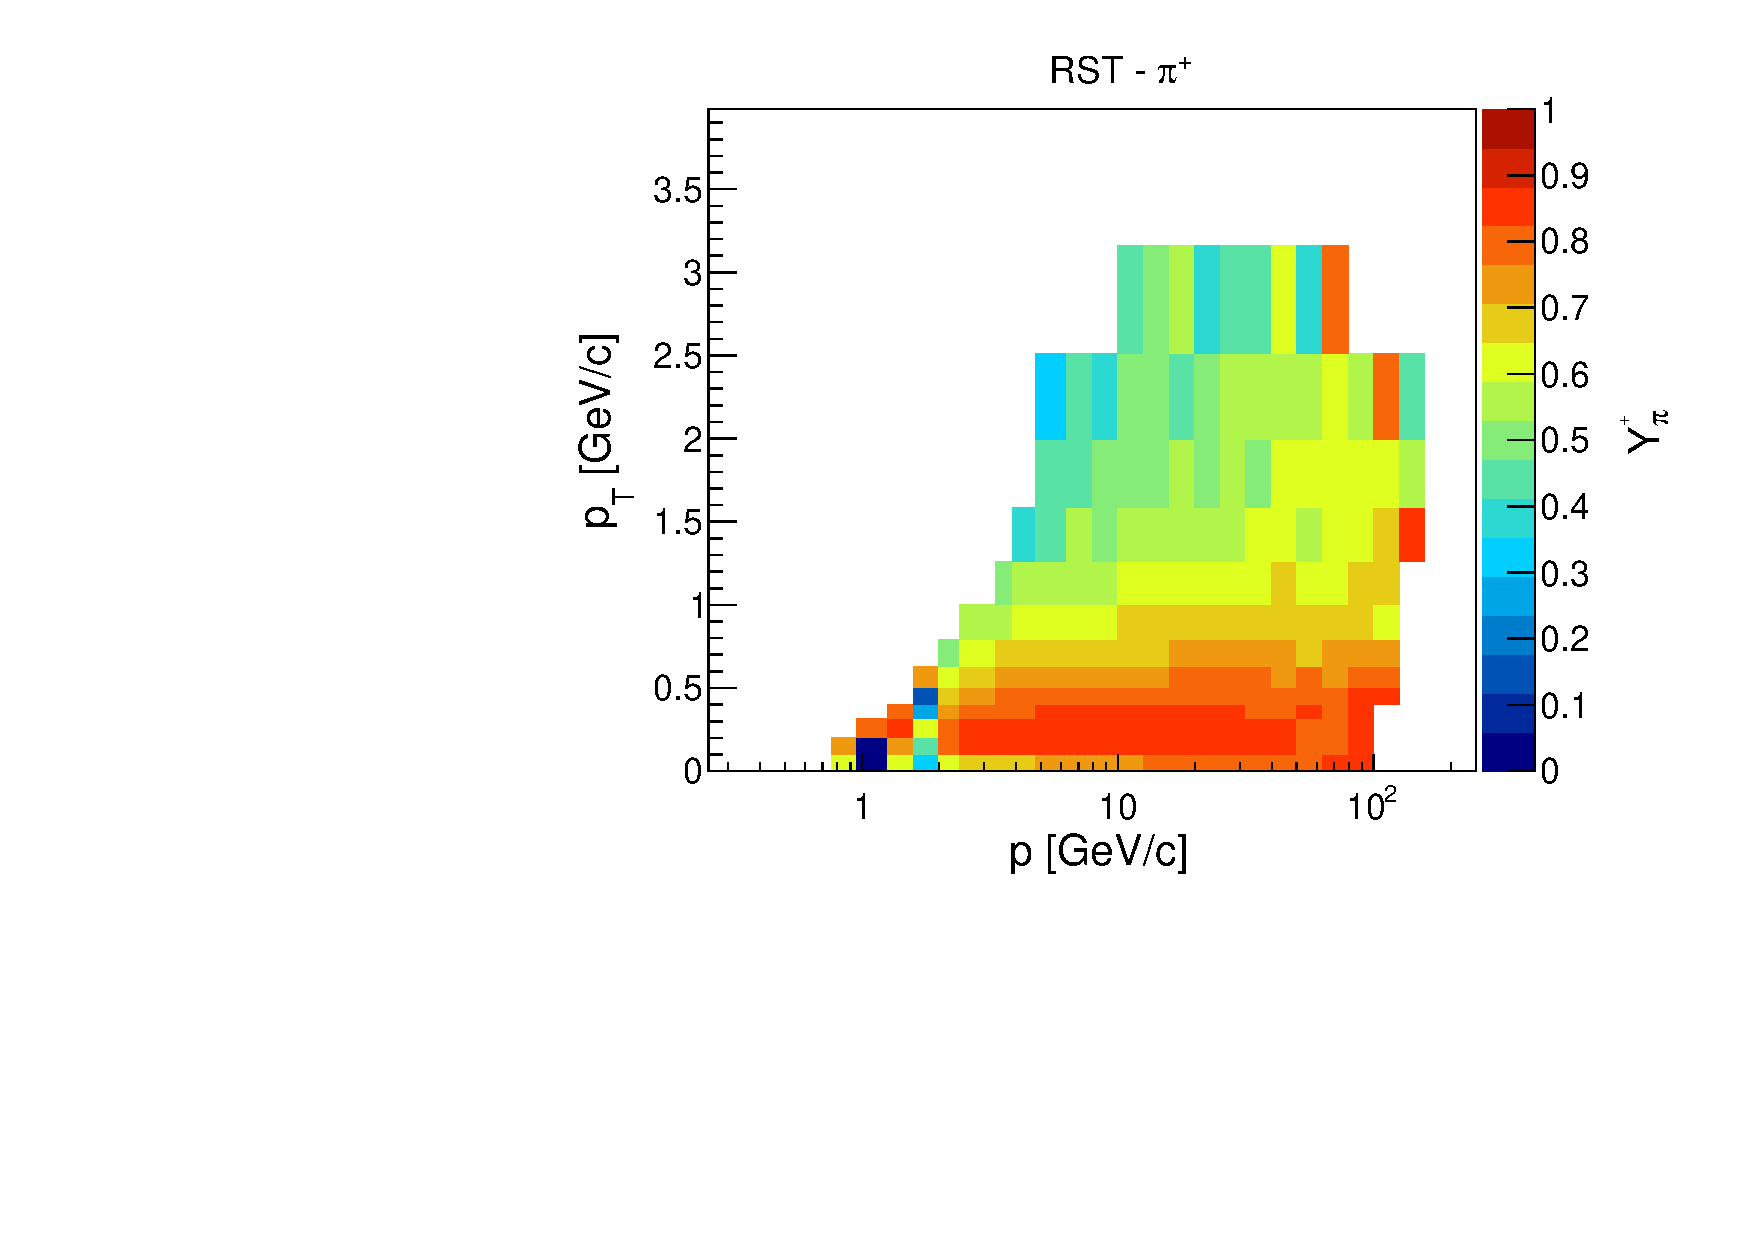
\includegraphics[clip, rviewport=0 0.13 1 0.94,width=0.4\textwidth]{dedx/fraction_350_fl0_v0_c1_p1}

  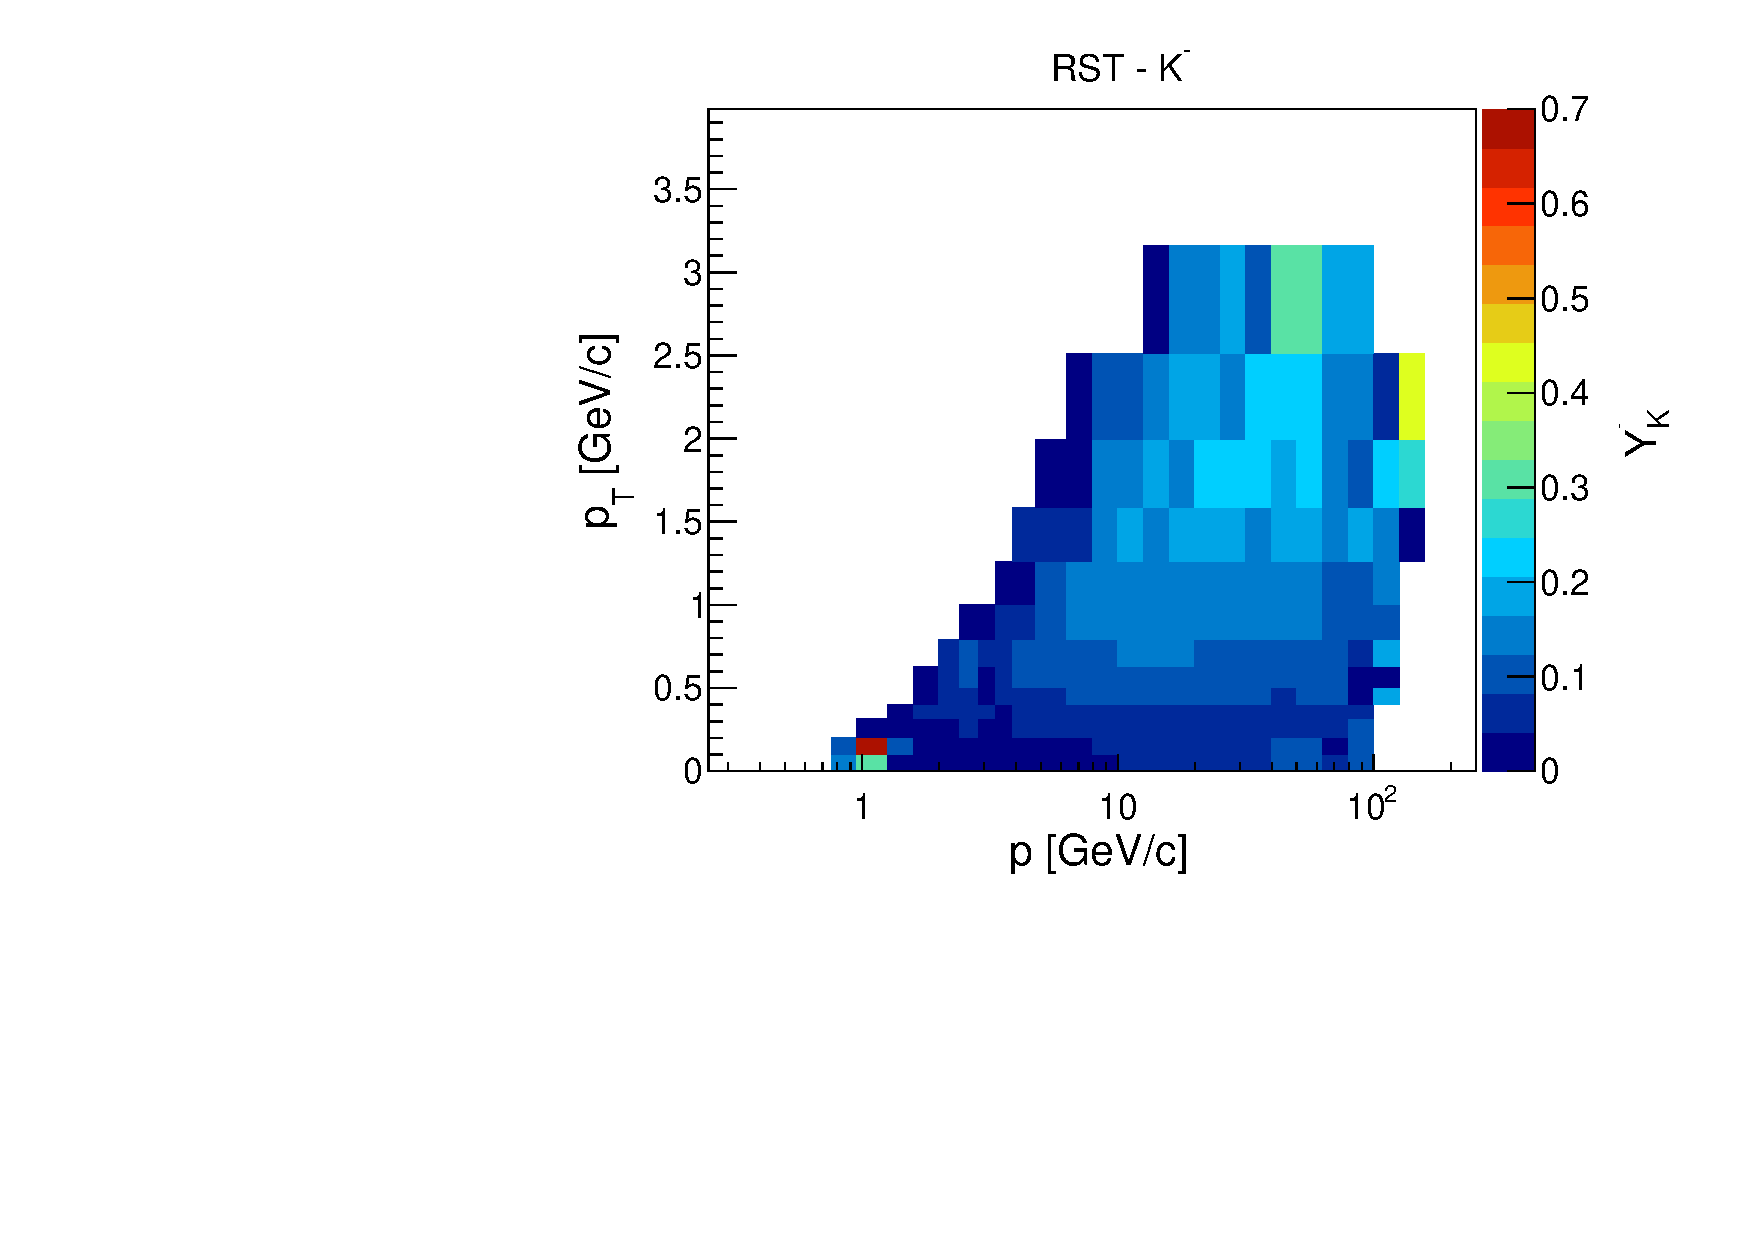
\includegraphics[clip, rviewport=0 0.13 1 0.94,width=0.4\textwidth]{dedx/fraction_350_fl0_v0_c0_p2}
  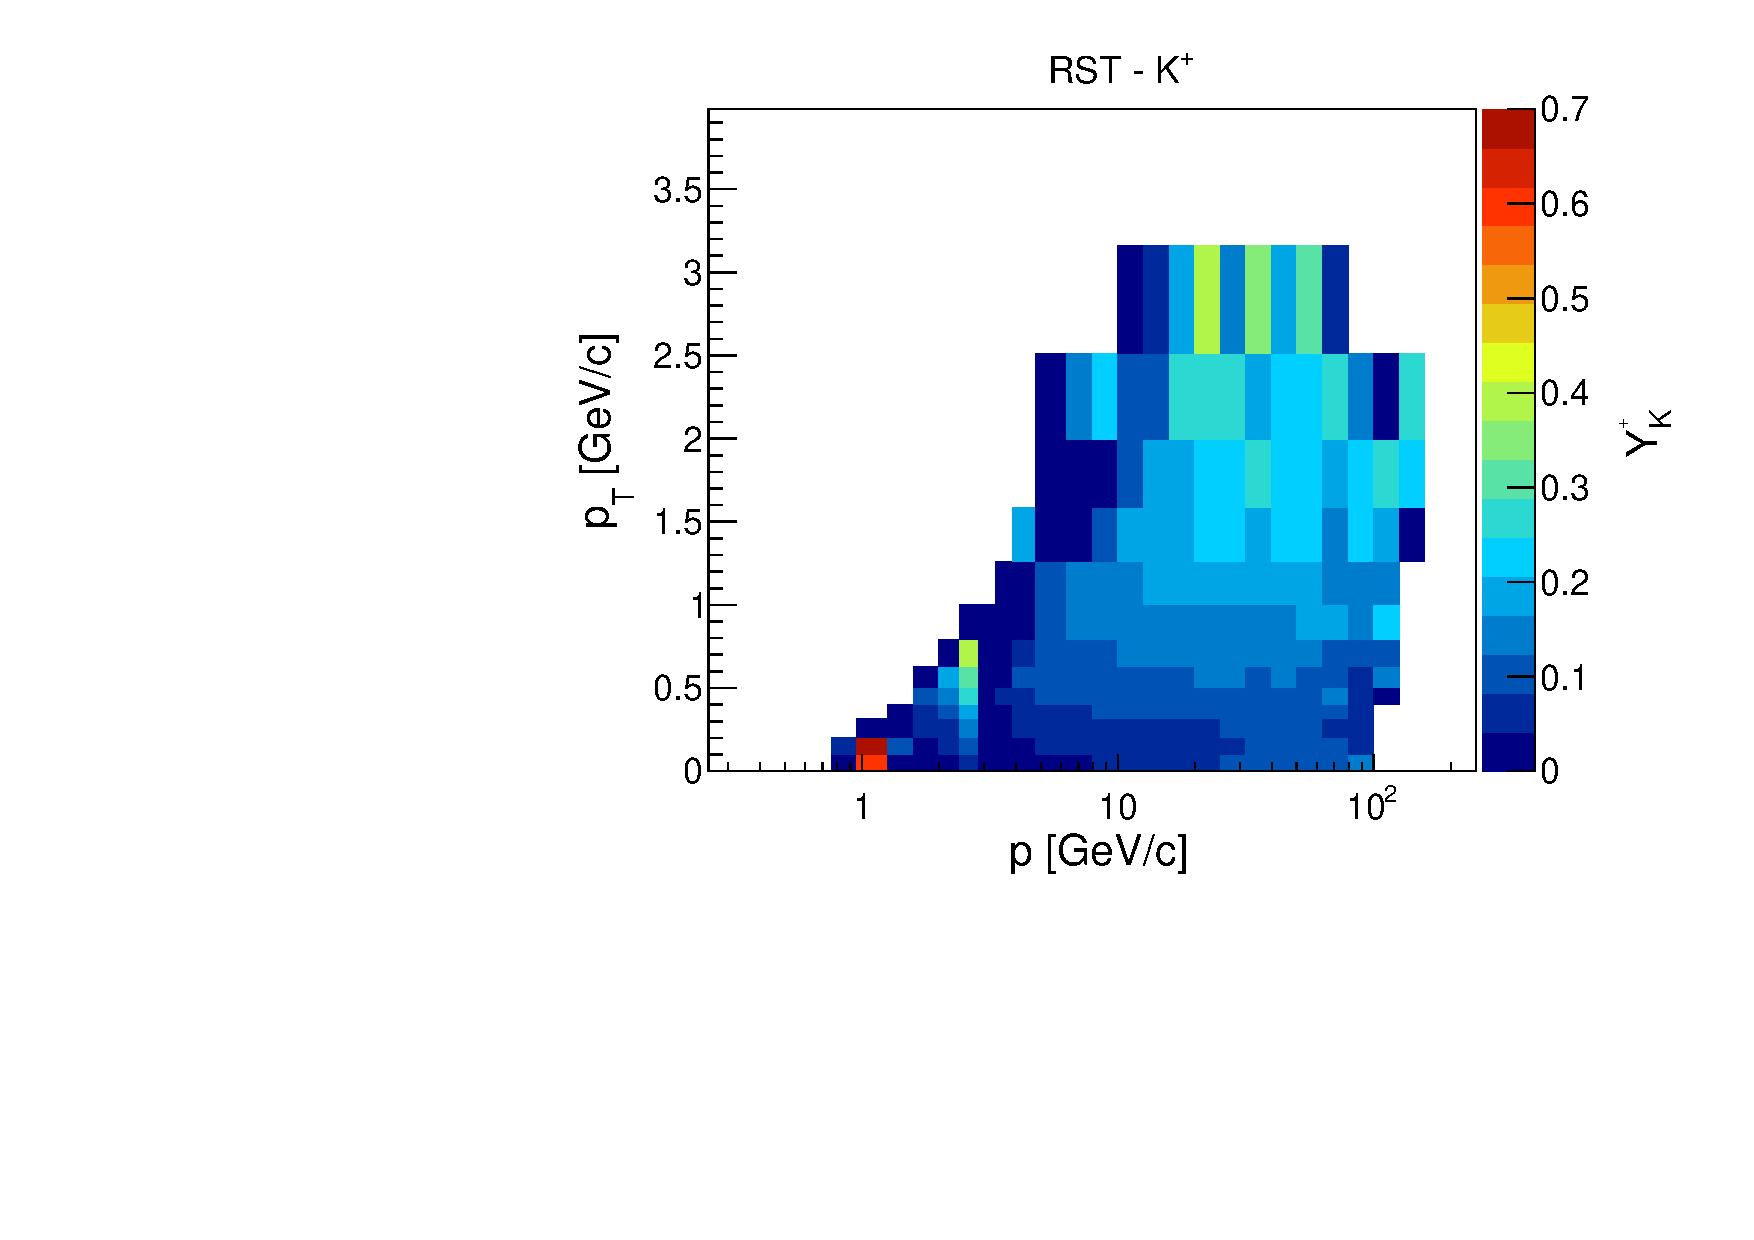
\includegraphics[clip, rviewport=0 0.13 1 0.94,width=0.4\textwidth]{dedx/fraction_350_fl0_v0_c1_p2}


  \includegraphics[clip, rviewport=0 0.13 1 0.94,width=0.4\textwidth]{dedx/fraction_350_fl0_v0_c0_p3}
  \includegraphics[clip, rviewport=0 0.13 1 0.94,width=0.4\textwidth]{dedx/fraction_350_fl0_v0_c1_p3}

  \includegraphics[clip, rviewport=0 0 1 0.94,width=0.4\textwidth]{dedx/fraction_350_fl0_v0_c0_p4}
  \includegraphics[clip, rviewport=0 0 1 0.94,width=0.4\textwidth]{dedx/fraction_350_fl0_v0_c1_p4}

  \caption{Particle fractions obtained from the fit of the RST dataset at 350 \GeVc.}
  \label{fig:hadron:dedx:fit:frac350r}
\end{figure}

%%%%%%%%%% FRACTIONS %%%%%%%%%%%%%%
\begin{figure}
  \centering
  \includegraphics[clip, rviewport=0 0.13 1 0.94,width=0.4\textwidth]{dedx/fraction_350_fl0_v1_c0_p0}
  \includegraphics[clip, rviewport=0 0.13 1 0.94,width=0.4\textwidth]{dedx/fraction_350_fl0_v1_c1_p0}

  \includegraphics[clip, rviewport=0 0.13 1 0.94,width=0.4\textwidth]{dedx/fraction_350_fl0_v1_c0_p1}
  \includegraphics[clip, rviewport=0 0.13 1 0.94,width=0.4\textwidth]{dedx/fraction_350_fl0_v1_c1_p1}

  \includegraphics[clip, rviewport=0 0.13 1 0.94,width=0.4\textwidth]{dedx/fraction_350_fl0_v1_c0_p2}
  \includegraphics[clip, rviewport=0 0.13 1 0.94,width=0.4\textwidth]{dedx/fraction_350_fl0_v1_c1_p2}


  \includegraphics[clip, rviewport=0 0.13 1 0.94,width=0.4\textwidth]{dedx/fraction_350_fl0_v1_c0_p3}
  \includegraphics[clip, rviewport=0 0.13 1 0.94,width=0.4\textwidth]{dedx/fraction_350_fl0_v1_c1_p3}

  \includegraphics[clip, rviewport=0 0 1 0.94,width=0.4\textwidth]{dedx/fraction_350_fl0_v1_c0_p4}
  \includegraphics[clip, rviewport=0 0 1 0.94,width=0.4\textwidth]{dedx/fraction_350_fl0_v1_c1_p4}

  \caption{Particle fractions obtained from the fit of the WST dataset at 350 \GeVc.}
  \label{fig:hadron:dedx:fit:frac350w}
\end{figure}

\clearpage



%%%%%%%%%% FAKE REL SIG %%%%%%%%%%%%%%
\begin{figure}
  \centering
  \includegraphics[clip, rviewport=0 0.13 1 0.94,width=0.4\textwidth]{dedx/fake_rel_sig_158_fl0_v1_c0_p1}
  \includegraphics[clip, rviewport=0 0.13 1 0.94,width=0.4\textwidth]{dedx/fake_rel_sig_158_fl0_v1_c1_p1}

  \includegraphics[clip, rviewport=0 0.13 1 0.94,width=0.4\textwidth]{dedx/fake_rel_sig_158_fl0_v1_c0_p2}
  \includegraphics[clip, rviewport=0 0.13 1 0.94,width=0.4\textwidth]{dedx/fake_rel_sig_158_fl0_v1_c1_p2}

  \includegraphics[clip, rviewport=0 0 1 0.94,width=0.4\textwidth]{dedx/fake_rel_sig_158_fl0_v1_c0_p3}
  \includegraphics[clip, rviewport=0 0 1 0.94,width=0.4\textwidth]{dedx/fake_rel_sig_158_fl0_v1_c1_p3}

  \caption{Relative standard deviation of the particle fractions obtained with SDEs for WST and 158 \GeVc dataset.}
  \label{fig:hadron:dedx:fit:fake:relsig158w}
\end{figure}



%%%%%%%%%% FAKE REL SIG %%%%%%%%%%%%%%
\begin{figure}
  \centering
  \includegraphics[clip, rviewport=0 0.13 1 0.94,width=0.4\textwidth]{dedx/fake_rel_sig_350_fl0_v0_c0_p1}
  \includegraphics[clip, rviewport=0 0.13 1 0.94,width=0.4\textwidth]{dedx/fake_rel_sig_350_fl0_v0_c1_p1}

  \includegraphics[clip, rviewport=0 0.13 1 0.94,width=0.4\textwidth]{dedx/fake_rel_sig_350_fl0_v0_c0_p2}
  \includegraphics[clip, rviewport=0 0.13 1 0.94,width=0.4\textwidth]{dedx/fake_rel_sig_350_fl0_v0_c1_p2}

  \includegraphics[clip, rviewport=0 0 1 0.94,width=0.4\textwidth]{dedx/fake_rel_sig_350_fl0_v0_c0_p3}
  \includegraphics[clip, rviewport=0 0 1 0.94,width=0.4\textwidth]{dedx/fake_rel_sig_350_fl0_v0_c1_p3}


  \caption{Relative standard deviation of the particle fractions obtained with SDEs for RST and 350 \GeVc dataset.}
  \label{fig:hadron:dedx:fit:fake:relsig350r}
\end{figure}

%%%%%%%%%% FAKE REL SIG %%%%%%%%%%%%%%
\begin{figure}
  \centering
  \includegraphics[clip, rviewport=0 0.13 1 0.94,width=0.4\textwidth]{dedx/fake_rel_sig_350_fl0_v1_c0_p1}
  \includegraphics[clip, rviewport=0 0.13 1 0.94,width=0.4\textwidth]{dedx/fake_rel_sig_350_fl0_v1_c1_p1}

  \includegraphics[clip, rviewport=0 0.13 1 0.94,width=0.4\textwidth]{dedx/fake_rel_sig_350_fl0_v1_c0_p2}
  \includegraphics[clip, rviewport=0 0.13 1 0.94,width=0.4\textwidth]{dedx/fake_rel_sig_350_fl0_v1_c1_p2}

  \includegraphics[clip, rviewport=0 0 1 0.94,width=0.4\textwidth]{dedx/fake_rel_sig_350_fl0_v1_c0_p3}
  \includegraphics[clip, rviewport=0 0 1 0.94,width=0.4\textwidth]{dedx/fake_rel_sig_350_fl0_v1_c1_p3}

  \caption{Relative standard deviation of the particle fractions obtained with SDEs for WST and 350 \GeVc dataset.}
  \label{fig:hadron:dedx:fit:fake:relsig350w}
\end{figure}


%%%%%%%%%% FAKE REL DEV %%%%%%%%%%%%%%
\begin{figure}
  \centering
  \includegraphics[clip, rviewport=0 0.13 1 0.94,width=0.4\textwidth]{dedx/fake_rel_dev_158_fl0_v1_c0_p1}
  \includegraphics[clip, rviewport=0 0.13 1 0.94,width=0.4\textwidth]{dedx/fake_rel_dev_158_fl0_v1_c1_p1}

  \includegraphics[clip, rviewport=0 0.13 1 0.94,width=0.4\textwidth]{dedx/fake_rel_dev_158_fl0_v1_c0_p2}
  \includegraphics[clip, rviewport=0 0.13 1 0.94,width=0.4\textwidth]{dedx/fake_rel_dev_158_fl0_v1_c1_p2}

  \includegraphics[clip, rviewport=0 0 1 0.94,width=0.4\textwidth]{dedx/fake_rel_dev_158_fl0_v1_c0_p3}
  \includegraphics[clip, rviewport=0 0 1 0.94,width=0.4\textwidth]{dedx/fake_rel_dev_158_fl0_v1_c1_p3}

  \caption{Average relative bias of the particle fractions obtained with SDEs for WST and 158 \GeVc dataset.}
  \label{fig:hadron:dedx:fit:fake:reldev158w}
\end{figure}



%%%%%%%%%% FAKE REL DEV %%%%%%%%%%%%%%
\begin{figure}
  \centering
  \includegraphics[clip, rviewport=0 0.13 1 0.94,width=0.4\textwidth]{dedx/fake_rel_dev_350_fl0_v0_c0_p1}
  \includegraphics[clip, rviewport=0 0.13 1 0.94,width=0.4\textwidth]{dedx/fake_rel_dev_350_fl0_v0_c1_p1}

  \includegraphics[clip, rviewport=0 0.13 1 0.94,width=0.4\textwidth]{dedx/fake_rel_dev_350_fl0_v0_c0_p2}
  \includegraphics[clip, rviewport=0 0.13 1 0.94,width=0.4\textwidth]{dedx/fake_rel_dev_350_fl0_v0_c1_p2}

  \includegraphics[clip, rviewport=0 0 1 0.94,width=0.4\textwidth]{dedx/fake_rel_dev_350_fl0_v0_c0_p3}
  \includegraphics[clip, rviewport=0 0 1 0.94,width=0.4\textwidth]{dedx/fake_rel_dev_350_fl0_v0_c1_p3}


  \caption{Average relative bias of the particle fractions obtained with SDEs for RST and 350 \GeVc dataset.}
  \label{fig:hadron:dedx:fit:fake:reldev350r}
\end{figure}

%%%%%%%%%% FAKE REL DEV %%%%%%%%%%%%%%
\begin{figure}
  \centering
  \includegraphics[clip, rviewport=0 0.13 1 0.94,width=0.4\textwidth]{dedx/fake_rel_dev_350_fl0_v1_c0_p1}
  \includegraphics[clip, rviewport=0 0.13 1 0.94,width=0.4\textwidth]{dedx/fake_rel_dev_350_fl0_v1_c1_p1}

  \includegraphics[clip, rviewport=0 0.13 1 0.94,width=0.4\textwidth]{dedx/fake_rel_dev_350_fl0_v1_c0_p2}
  \includegraphics[clip, rviewport=0 0.13 1 0.94,width=0.4\textwidth]{dedx/fake_rel_dev_350_fl0_v1_c1_p2}

  \includegraphics[clip, rviewport=0 0 1 0.94,width=0.4\textwidth]{dedx/fake_rel_dev_350_fl0_v1_c0_p3}
  \includegraphics[clip, rviewport=0 0 1 0.94,width=0.4\textwidth]{dedx/fake_rel_dev_350_fl0_v1_c1_p3}

  \caption{Average relative bias of the particle fractions obtained with SDEs for WST and 350 \GeVc dataset.}
  \label{fig:hadron:dedx:fit:fake:reldev350w}
\end{figure}

\clearpage


%%%%%%%%%% COR %%%%%%%%%%%%%%
\begin{figure}
  \centering
  \includegraphics[clip, rviewport=0 0.13 1 0.94,width=0.4\textwidth]{dedx/cor_158_v1_c0_p1}
  \includegraphics[clip, rviewport=0 0.13 1 0.94,width=0.4\textwidth]{dedx/cor_158_v1_c1_p1}

  \includegraphics[clip, rviewport=0 0.13 1 0.94,width=0.4\textwidth]{dedx/cor_158_v1_c0_p2}
  \includegraphics[clip, rviewport=0 0.13 1 0.94,width=0.4\textwidth]{dedx/cor_158_v1_c1_p2}

  \includegraphics[clip, rviewport=0 0 1 0.94,width=0.4\textwidth]{dedx/cor_158_v1_c0_p3}
  \includegraphics[clip, rviewport=0 0 1 0.94,width=0.4\textwidth]{dedx/cor_158_v1_c1_p3}

  \caption{Correction factor for WST and 158 \GeVc dataset.}
  \label{fig:hadron:dedx:fit:fake:cor158w}
\end{figure}


%%%%%%%%%% COR %%%%%%%%%%%%%%
\begin{figure}
  \centering
  \includegraphics[clip, rviewport=0 0.13 1 0.94,width=0.4\textwidth]{dedx/cor_350_v0_c0_p1}
  \includegraphics[clip, rviewport=0 0.13 1 0.94,width=0.4\textwidth]{dedx/cor_350_v0_c1_p1}

  \includegraphics[clip, rviewport=0 0.13 1 0.94,width=0.4\textwidth]{dedx/cor_350_v0_c0_p2}
  \includegraphics[clip, rviewport=0 0.13 1 0.94,width=0.4\textwidth]{dedx/cor_350_v0_c1_p2}

  \includegraphics[clip, rviewport=0 0 1 0.94,width=0.4\textwidth]{dedx/cor_350_v0_c0_p3}
  \includegraphics[clip, rviewport=0 0 1 0.94,width=0.4\textwidth]{dedx/cor_350_v0_c1_p3}

  \caption{Correction factor for RST and 350 \GeVc dataset.}
  \label{fig:hadron:dedx:fit:fake:cor350r}
\end{figure}

%%%%%%%%%% COR %%%%%%%%%%%%%%
\begin{figure}
  \centering
  \includegraphics[clip, rviewport=0 0.13 1 0.94,width=0.4\textwidth]{dedx/cor_350_v1_c0_p1}
  \includegraphics[clip, rviewport=0 0.13 1 0.94,width=0.4\textwidth]{dedx/cor_350_v1_c1_p1}

  \includegraphics[clip, rviewport=0 0.13 1 0.94,width=0.4\textwidth]{dedx/cor_350_v1_c0_p2}
  \includegraphics[clip, rviewport=0 0.13 1 0.94,width=0.4\textwidth]{dedx/cor_350_v1_c1_p2}

  \includegraphics[clip, rviewport=0 0 1 0.94,width=0.4\textwidth]{dedx/cor_350_v1_c0_p3}
  \includegraphics[clip, rviewport=0 0 1 0.94,width=0.4\textwidth]{dedx/cor_350_v1_c1_p3}

  \caption{Correction factor for WST and 350 \GeVc dataset.}
  \label{fig:hadron:dedx:fit:fake:cor350w}
\end{figure}


\clearpage

%%%%%%%%%% FRACTION %%%%%%%%%%%%%%

\begin{figure}
  \centering
  \includegraphics[clip, rviewport=0 0 1 1,width=1.00\textwidth]{dedx/fraction_pt_158_fl2_v1}
  \caption{Particle fractions obtained from the \dedx fit of the WST and 158 \GeVc dataset, with target inserted.}
  \label{fig:hadron:dedx:fit:final158w}
\end{figure}

\begin{figure}
  \centering
  \includegraphics[clip, rviewport=0 0 1 1,width=1.00\textwidth]{dedx/fraction_pt_350_fl2_v0}
  \caption{Particle fractions obtained from the \dedx fit of the RST and 350 \GeVc dataset, with target inserted.}
  \label{fig:hadron:dedx:fit:final350r}
\end{figure}

\begin{figure}
  \centering
  \includegraphics[clip, rviewport=0 0 1 1,width=1.00\textwidth]{dedx/fraction_pt_350_fl2_v1}
  \caption{Particle fractions obtained from the \dedx fit of the WST and 350 \GeVc dataset, with target inserted.}
  \label{fig:hadron:dedx:fit:final350w}
\end{figure}

%%%%%%%%%% FRACTION OUT%%%%%%%%%%%%%%
\begin{figure}
  \centering
  \includegraphics[clip, rviewport=0 0 1 1,width=1.00\textwidth]{dedx/fraction_out_pt_158_v0}
  \caption{Particle fractions obtained from the \dedx fit of the RST and 158 \GeVc dataset, with target removed.}
  \label{fig:hadron:dedx:fit:out158r}
\end{figure}

\begin{figure}
  \centering
  \includegraphics[clip, rviewport=0 0 1 1,width=1.00\textwidth]{dedx/fraction_out_pt_158_v1}
  \caption{Particle fractions obtained from the \dedx fit of the WST and 158 \GeVc dataset, with target inserted.}
  \label{fig:hadron:dedx:fit:out158w}
\end{figure}

\begin{figure}
  \centering
  \includegraphics[clip, rviewport=0 0 1 1,width=1.00\textwidth]{dedx/fraction_out_pt_350_v0}
  \caption{Particle fractions obtained from the \dedx fit of the RST and 350 \GeVc dataset, with target inserted.}
  \label{fig:hadron:dedx:fit:out350r}
\end{figure}

\begin{figure}
  \centering
  \includegraphics[clip, rviewport=0 0 1 1,width=1.00\textwidth]{dedx/fraction_out_pt_350_v1}
  \caption{Particle fractions obtained from the \dedx fit of the WST and 350 \GeVc dataset, with target inserted.}
  \label{fig:hadron:dedx:fit:out350w}
\end{figure}



%%%%%%%%%%% DECAY DIST CUT %%%%%%%%%%%%%%%%%%
\begin{figure}
  \centering
  \includegraphics[clip, rviewport=0 0 1 1,width=0.99\textwidth]{vzero/cut_dist_Data350}
  
  \caption{Optimization of the \decaydistmin for the 350 \GeVc dataset. The plot on left, middle and right shows \lamb, \antilamb and \kzeros, respectively.}
  \label{fig:hadron:vzero:cuts:decaydist:350}
\end{figure}

\clearpage

%%%%%%%%%%% CHI SQ %%%%%%%%%%%%%%%%%%
\begin{figure}
  \centering
  \includegraphics[clip, rviewport=0 0 1 1,width=0.99\textwidth]{vzero/chisq_Data350_t0_ph1}
  
  \caption{}
  \label{fig:hadron:vzero:signal:chi:350}
\end{figure}


%%%%%%%%%%% EXTRACTED SIGNAL %%%%%%%%%%%%%%%%%%
\begin{figure}
  \centering
  \includegraphics[clip, rviewport=0 0 1 1,width=0.99\textwidth]{vzero/signal_Data350_t0}
  
  \caption{}
  \label{fig:hadron:vzero:signal:extracted:350in}
\end{figure}

%%%%%%%%%%% EXTRACTED SIGNAL %%%%%%%%%%%%%%%%%%
\begin{figure}
  \centering
  \includegraphics[clip, rviewport=0 0 1 1,width=0.99\textwidth]{vzero/signal_Data350_t1}
  
  \caption{}
  \label{fig:hadron:vzero:signal:extracted:350out}
\end{figure}


%%%%%%%%%%% DIST %%%%%%%%%%%%%%%%%%
\begin{figure}[!ht]
  \centering
  \includegraphics[clip, rviewport=0 0 1 1,width=0.32\textwidth]{vzero/mass_Data350_t0_ph1_h0_x1_y3}
  \includegraphics[clip, rviewport=0 0 1 1,width=0.32\textwidth]{vzero/mass_Data350_t0_ph1_h1_x1_y3}
  \includegraphics[clip, rviewport=0 0 1 1,width=0.32\textwidth]{vzero/mass_Data350_t0_ph1_h2_x2_y4}

  \vspace{0.5cm}
    
  \includegraphics[clip, rviewport=0 0 1 1,width=0.32\textwidth]{vzero/mass_Data350_t0_ph1_h0_x5_y0}
  \includegraphics[clip, rviewport=0 0 1 1,width=0.32\textwidth]{vzero/mass_Data350_t0_ph1_h1_x5_y0}
  \includegraphics[clip, rviewport=0 0 1 1,width=0.32\textwidth]{vzero/mass_Data350_t0_ph1_h2_x5_y1}

  
  \caption{Examples of the fitted \minv distributions for the 350 \GeVc dataset. The plot on left, middle and right shows \lamb, \antilamb and \kzeros, respectively.}
  \label{fig:hadron:vzero:signal:dist:350:in}
\end{figure}



%%%%%%%%%%% DIST %%%%%%%%%%%%%%%%%%
\begin{figure}[!ht]
  \centering
  \includegraphics[clip, rviewport=0 0 1 1,width=0.32\textwidth]{vzero/mass_Data350_t1_ph0_h0_x3_y0}
  \includegraphics[clip, rviewport=0 0 1 1,width=0.32\textwidth]{vzero/mass_Data350_t1_ph0_h1_x3_y0}
  \includegraphics[clip, rviewport=0 0 1 1,width=0.32\textwidth]{vzero/mass_Data350_t1_ph0_h2_x3_y0}
  
  \caption{Examples of the fitted \minv distributions for the 350 \GeVc dataset, with target removed. The plot on left, middle and right shows \lamb, \antilamb and \kzeros, respectively.}
  \label{fig:hadron:vzero:signal:dist:350:out}
\end{figure}


%%%%%%%%%% BETA %%%%%%%%%%%%%%
\begin{figure}
  \centering
  \includegraphics[clip, rviewport=0 0.13 1 0.94,width=0.4\textwidth]{dedx/fac_350_All_beta_c0_p1}
  \includegraphics[clip, rviewport=0 0.13 1 0.94,width=0.4\textwidth]{dedx/fac_350_All_beta_c1_p1}

  \includegraphics[clip, rviewport=0 0.13 1 0.94,width=0.4\textwidth]{dedx/fac_350_All_beta_c0_p2}
  \includegraphics[clip, rviewport=0 0.13 1 0.94,width=0.4\textwidth]{dedx/fac_350_All_beta_c1_p2}

  \includegraphics[clip, rviewport=0 0.13 1 0.94,width=0.4\textwidth]{dedx/fac_350_All_beta_c0_p3}
  \includegraphics[clip, rviewport=0 0.13 1 0.94,width=0.4\textwidth]{dedx/fac_350_All_beta_c1_p3}

  \caption{$\beta$ correction factor for the 350 \GeVc dataset.}
  \label{fig:hadron:correction:beta:dedx350}
\end{figure}


%%%%%%%%%%% BETA %%%%%%%%%%%%%%%%%%
\begin{figure}
  \centering
  \includegraphics[clip, rviewport=0 0 1 1,width=0.95\textwidth]{vzero/beta350}
  
  \caption{$\beta$ correction factor for the 350 \GeVc dataset.}
  \label{fig:hadron:correction:beta:vzero350}
\end{figure}

